\documentclass[a4paper,oneside,12pt]{book}
%----------------------------------------------------------------------------------------
%	WELCOME!
%   It's probably worth having a read through this file to set up the broad parameters.
%----------------------------------------------------------------------------------------

%----------------------------------------------------------------------------------------
%	COVER PAGE
%   The cover page is laid out in title/title.tex. You can choose a colour
%   or black and white logo
%----------------------------------------------------------------------------------------

%----------------------------------------------------------------------------------------
%	THESIS INFORMATION
%   Put title, author name, degree, type of work, school, department in here
%   It will be used for the title page and for the embedded PDF information
%----------------------------------------------------------------------------------------

\newcommand{\thesistitle}{The Impact of Synthetic Data On The Reliability of Hand Tracking Systems} % Your thesis title, this is used in the title and abstract
\newcommand{\degree}{MAI (Computer Engineering)} % Your degree name, this is used in the title page and abstract
\newcommand{\typeofthesis}{dissertation} % dissertation, Final Year Project, report, etc.
\newcommand{\authorname}{Daniel Desmond Dennis} % Your name, this is used in the title page and PDF stuff
%% Comment out the next line if you don't want your ID to appear
\newcommand{\authorid}{15316947} % Your ID
\newcommand{\keywords}{this, that, more} % Keywords for your thesis
\newcommand{\school}{\href{http://www.scss.tcd.ie}{School of Computer Science and Statistics}} % Your school's name and URL, this is used in the title page

%% Comment out the next line if you don't want a department to appear
%\newcommand{\department}{\href{http://researchgroup.university.com}{Department Name}} % Your research group's name and URL, this is used in the title page

\AtBeginDocument{
\hypersetup{pdftitle=\thesistitle} % Set the PDF's title to your title
\hypersetup{pdfauthor=\authorname} % Set the PDF's author to your name
\hypersetup{pdfkeywords=\keywords} % Set the PDF's keywords to your keywords
\hypersetup{pdfsubject=\degree} % Set the PDF's keywords to your keywords
}

\usepackage[table]{xcolor}

%% Language and font encodings
\usepackage[T1]{fontenc} 
\usepackage[utf8]{inputenc}
\usepackage[english]{babel}

%% Bibliographical stuff
\usepackage[square,sort,comma,numbers]{natbib}

%% Document size
% include showframe as an option if you want to see the boxes
\usepackage[a4paper,top=2.54cm,bottom=2.54cm,left=2.54cm,right=2.54cm,headheight=16pt]{geometry}
\renewcommand{\baselinestretch}{1.4} 
% \usepackage[margin=20mm, bindingoffset=15mm]{geometry}

%% Useful packages
\usepackage{amsmath}
\usepackage[autostyle=true]{csquotes} % Required to generate language-dependent quotes in the bibliography
\usepackage[pdftex]{graphicx}
\usepackage[colorinlistoftodos]{todonotes}
\usepackage[colorlinks=true, allcolors=black]{hyperref}
\usepackage{caption} % if no caption, no colon
% \usepackage{sfmath} %use sans-serif in the maths sections too
\usepackage[parfill]{parskip}    % Begin paragraphs with an empty line rather than an indent
\usepackage{setspace} % to permit one-and-a-half or double spacing
\usepackage{enumerate} % fancy enumerations like (i) (ii) or (a) (b) and suchlike
% \usepackage{booktabs} % To thicken table lines
\usepackage{fancyhdr}
\usepackage{amssymb}
\usepackage{bm}
\usepackage{mathrsfs}

% \usepackage{xcolor}
\usepackage{siunitx}
\usepackage{afterpage}
\usepackage{multirow}
\usepackage{diagbox}
\usepackage{placeins}
\usepackage{float}


% \usepackage{listings}
% \lstset{
%   basicstyle=\linespread{0.94}\ttfamily,
% %   columns=fullflexible,
% %   frame=single,
%   breaklines=true,
%   postbreak=\mbox{\textcolor{red}{$\hookrightarrow$}\space},
%   numbers=left,
% }
% \let\Oldsubsection\subsection
% \renewcommand{\subsection}{\FloatBarrier\subsection}

\pagestyle{plain} % Embrace simplicity!

%% It is not a requirement of the university that the font should be sans-serif, but
%% the Mechanical engineers require it. Comment out the following line to disable it
% \renewcommand{\familydefault}{\sfdefault} %use the sans-serif font as default

%% If you're not using sans-serif, consider using Palatino instead of the LaTeX standard
% \usepackage{mathpazo} % Use the Palatino font by default if you prefer it to Computer Modern

\renewcommand{\theequation}{\arabic{equation}} %% use continuous equation numbers

%% Format Chapter headings appropriately
\usepackage{titlesec}
\titleformat{\chapter}[hang] 
{\normalfont\huge\bfseries}{\thechapter}{1cm}{} 

\title{\thesistitle}
\author{\authorname}

% % Uncomment this for a dark-themed document
% \definecolor{darkgrey}{rgb}{0.117,0.117,0.117}
% \definecolor{lightgrey}{rgb}{0.828,0.828,0.828}
% \pagecolor{darkgrey}
% \color{lightgrey}

\frontmatter
\begin{document}
\begin{titlepage}

\center % Center everything on the page

%% All the text parameters should be taken from the start of the main.tex file.
%% You should only alter stuff here if you want to change the layout

%----------------------------------------------------------------------------------------
%	LOGO SECTION
%----------------------------------------------------------------------------------------
%% Choose one of the following -- a colour or black-and-white logo


\includegraphics{title/Trinity_RGB_transparent_main.png}\\[1cm] 
%\includegraphics[width=12cm]{title/black-stacked-trinity.jpg}\\[1cm] 

\Large \school\\[1.2cm] % Minor heading such as course title
\ifdefined\department
\large \department\\[1.2cm] % Minor heading such as course title
\fi

%----------------------------------------------------------------------------------------
%	TITLE SECTION
%----------------------------------------------------------------------------------------
\makeatletter
{ \huge \bfseries \thesistitle}\\[1.2cm] % Title of your document

% { \huge \bfseries \textcolor{red}{DRAFT}}
 

%----------------------------------------------------------------------------------------
%	AUTHOR SECTION
%----------------------------------------------------------------------------------------

\ifdefined\authorid
\authorname\\ % Your name
\authorid\\[1.4cm] % Your Student ID
\else
\authorname\\[1.4cm] % Your name
\fi

%----------------------------------------------------------------------------------------
%	DATE SECTION
%----------------------------------------------------------------------------------------

{\large April 2020}\\[1.4cm] % Date, change the \today to a set date if you want to be precise
\vspace{2cm}
 
%----------------------------------------------------------------------------------------
%	TYPE OF THESIS SECTION
%----------------------------------------------------------------------------------------
 A \typeofthesis\ submitted in partial fulfilment\\of the requirements for the degree of\\
\degree

\vfill % Fill the rest of the page with whitespace

\end{titlepage}
\pagenumbering{roman}
\section*{\Huge{Declaration}}
\vspace{2.5cm}
I hereby declare that this project is entirely my own work and that it has not been submitted as an exercise for a degree at this or any other university

% \vspace{1cm}
% I have read and I understand the plagiarism provisions in the General Regulations of the University Calendar for the current year, found at \url{http://www.tcd.ie/calendar}.
% \vspace{1cm}

% I have also completed the Online Tutorial on avoiding plagiarism `Ready Steady Write', located at
% \url{http://tcd-ie.libguides.com/plagiarism/ready-steady-write}.
\vspace{5cm}

Signed:~\rule{5cm}{0.3pt}\hfill Date:~\rule{5cm}{0.3pt}
\chapter{Abstract}

This dissertation investigates the merits of using synthetic data for training a hand tracking model to address the problem of the lack of training data for such systems. This is achieved by looking at two different synthetic data generation strategies, and training an existing hand tracking model to see how it performs on those generated synthetic datasets. An existing real dataset, the MSRA dataset is used as a control. The MANO model is used as the basis for generating synthetic data, and V2V-Posenet is used as the existing hand tracking model. The first strategy generates the data based on random parameters for MANO, this is referred to as the {\slshape Random MANO Dataset}. The second strategy generates the data based on parameters determined from the groundtruth of the real dataset to recreate that real dataset using inverse kinematics, this is referred to as the {\slshape IK MANO Dataset}.

In recent years, the accuracy of hand tracking systems has improved with the use of {\slshape convolutional neural networks} (CNNs). However, these systems need comprehensive training data, and such a dataset does not exist currently. This need is underlined by the fact that current hand tracking systems do not generalise well for a given training dataset, and performs poorly for hand poses that are not covered by that training dataset. The reasons for this lack of data are twofold. Firstly, annotating these datasets is difficult. Secondly, the human hand is a uniquely complex object, and a comprehensive dataset needs to cover a diverse range of; camera perspectives, hand poses, hand shapes, and interactions with objects, so the amount of data that needs to be collected to cover these ranges is also unknown. Synthetic data offers a way around this issue, since the annotation is theoretically perfect, and the capture of that data can be automated.

This dissertation shows that generating synthetic based on the {\slshape Random MANO Dataset} strategy shows promise, but more testing is required by generating more synthetic images. State-of-the-art results on this test dataset is demonstrated at an 8.90mm average per-joint mean squared error, but poor performance when comparing with the real test dataset. It also shows that trying to recreate a real dataset with the {\slshape IK MANO Dataset} is challenging, with efforts to achieve this showing poor performance at 77.44mm. The key contributions of this dissertation are (1) performing a side-by-side comparison between a synthetic and real hand tracking dataset using the state-of-the-art synthetic hand data generation method, MANO, (2) giving the basis for a new synthetic dataset based on the MANO model with the {\slshape Random MANO Dataset}, and (3) providing a new framework for generating a synthetic dataset by using a real dataset as a basis with the {\slshape IK MANO Dataset}.

\newpage
% \onehalfspacing\raggedright %\raggedright turns off justification and hypenation

\section*{\Huge{Acknowledgements}}
Thank you to my supervisor, Dr Gerard Lacey who guided me through this project and provided invaluable advice. Thank you to Tejo Chalasani who also provided helpful advice on hand tracking, and was always available for help if I had a problem. Thank you to Yalong Li ({\slshape dragonbook} on GitHub) whose PyTorch implementation of the V2V-PoseNet network was central to the experimental setup of this project. Thank you to Xinghao Chen ({\slshape xinghaochen} on GitHub) who hosts a comprehensive list of papers and other works related to hand tracking. Thank you to my father Gus, as well as friends Alec Barber and Davy Nash, who exposed the most egregious errors and omissions in assisting the editing process of this document. Thank you to Dr Mike Brady for providing the \LaTeX template for this document. Finally, thank you to the many people on Stack Exchange websites (mostly Stack Overflow and \TeX) as well as other assorted websites who have already asked and answered many of the questions I had in relation to this project and beyond.
\tableofcontents
\listoffigures
\listoftables
\newpage
\section*{\Huge{Nomenclature}}
\begin{tabular}{ll}
% A&Area of the wing&$m^{2}$\\
% B\\
% C& Roman letters first, with capitals\ldots\\
% a&then lower case.\\
% b\\
% c\\
% $\Gamma$&Followed by Greek capitals\ldots\\
% $\alpha$&then lower case greek symbols.\\
% $\beta$\\
% $\epsilon$\\
% TLA&Finally, three letter acronyms and other abbreviations arranged alphabetically\\
CNN & Convolutional Neural Network \\
FCN & Fully Convolutional Neural Network \\
LBS & Linear Blend Skinning \\
MSE & Mean Square Error \\
ROI & Region Of Interest \\
&\\
% $\bm{Z}_{m,n}$ & Individual pixel from a depthmap image\\
$\bm{\mathrm{D}}^t$ & Training dataset, where $\bm{\mathrm{D}}^t_k\in\bm{Z}$\\
$\bm{\mathrm{D}}^v$ & Test dataset, where $\bm{\mathrm{D}}^v_k\in\bm{Z}$\\
$E$ & Performance metric \\
$\bm{v}$ & 3D centre of hand in depthmap image $\bm{Z}$, where $\bm{v}\in \mathbb{R}^3$\\
$\bm{\mathrm{Y}}^{i}$ & Groundtruth hand joints, where $\bm{\mathrm{Y}}^{i}_{n} \equiv \bm{\Phi}$, $\bm{\mathrm{Y}}^{i}_{n,m} \equiv \bm{\Phi}_{m}$\\
$\bm{\mathrm{Y}}^{o}$ & Predicted hand joints, where $\bm{\mathrm{Y}}^{o}_{n} \equiv \bm{\Phi}$, $\bm{\mathrm{Y}}^{o}_{n,m} \equiv \bm{\Phi}_{m}$\\
$\bm{Z}$ & Depthmap image, where $\bm{Z}_{m,n} \in \mathbb{N}$ \\

$\bm{\beta}$ & MANO Hand shape parameter, where $\bm{\beta} \in \mathbb{R}^{10}$ \\
$\bm{\theta}$ & MANO hand pose parameter, where $\bm{\theta} \in \mathbb{R}^{45}$\\
$\bm{\Phi}$ & Hand joints, where \bm{$\Phi}=\{\bm{\Phi}_1, \bm{\Phi}_2, ..., \bm{\Phi}_N\}, \bm{\Phi}_{n} \in \mathbb{R}^{3}$\\
&\\
$a$& A scalar value\\
$\bm{a}$ & A vector value\\
$\bm{A}$ & A matrix value\\
$\bm{\mathrm{A}}$ & A tensor value\\
&\\
Articulation & The particular position of the fingers of a hand with respect to each other.\\
Annotation & The marked groundtruth for a depthmap $\bm{Z}$.\\
Groundtruth & True value for $N$ keypoints.\\
Joint & A type of keypoint.\\
Keypoint & Known reference point in a hand in 3D cartesian space.\\
Point Cloud & A series of 3D points which together describe the shape of a 3D surface.\\
Pose & An alternative name for articulation.\\
Prediction & Prediction of the keypoints from a hand tracking model.\\
&\\
\end{tabular}\\
{\bfseries All notation follows the convention set by \cite{goodfellow2016deep}.}

\section*{\Huge{Conventions}}

\begin{figure}[h]
    \renewcommand\thefigure{0.1}
    \centering
    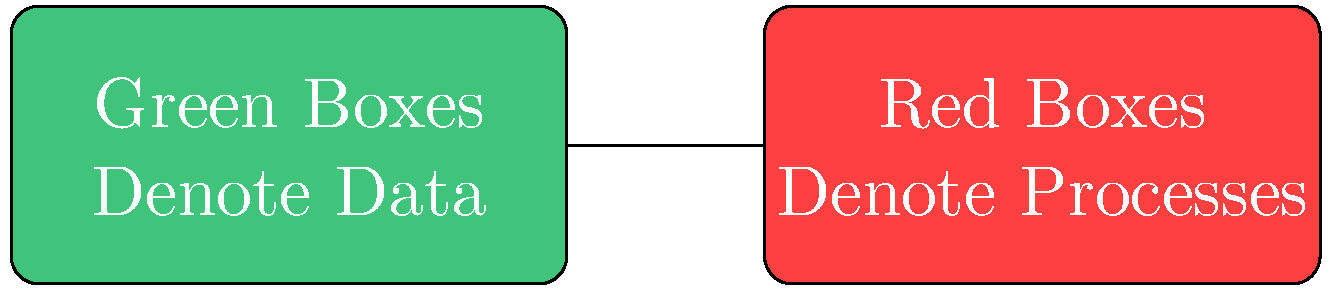
\includegraphics[width=0.5\linewidth]{figs/general/box_standard.pdf}
    \caption{Box diagram convention. All boxes flow from left to right. Green boxes denote data, and red boxes denote a process on that data.}
\end{figure}

\begin{figure}[h]
    \renewcommand\thefigure{0.2}
    \centering
    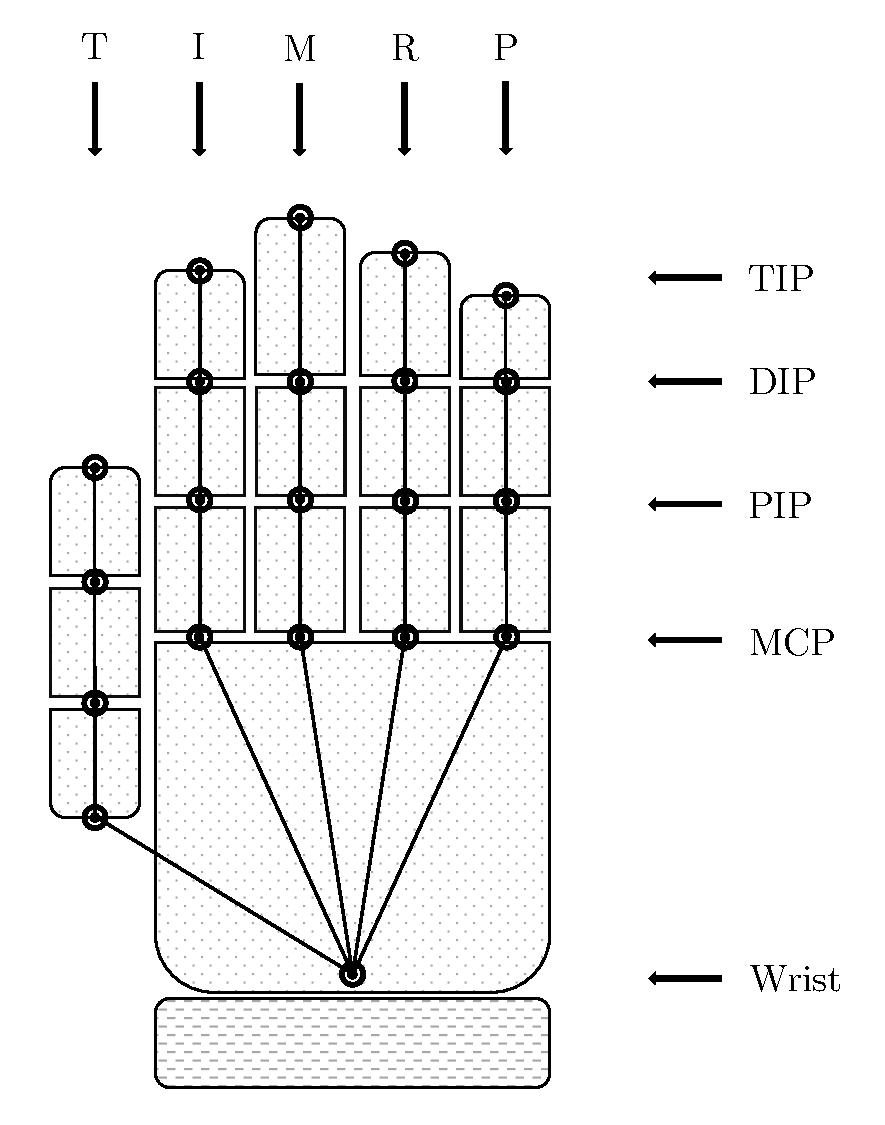
\includegraphics[width=250px]{figs/general/hand_schematic.pdf}
    \caption{Schematic of hand and keypoints. The goal of a hand tracking system is to predict the 3D locations of these keypoints. A keypoint name is the combination of the finger name and joint type, for example, the MCP joint of the Index finger is called the IMCP keypoint. Each of these keypoint names has an equivalent index in $\bm{\Phi}$. From left to right, the finger names used are: thumb, index, middle, ring, and pinky.}
    \label{fig:sd:hand}
    \end{figure}

\vspace{2cm}

% Point cloud?
% Grountruth

% If a parameter has a typical unit that is used throughout your report, then it should be included here on the right hand side.

% If you have a very mathematical report, then you may wish to divide the nomenclature list into functions and variables, and then sub- and super-scripts.

% Note that Roman mathematical symbols are typically in a serif font in italics.

\mainmatter
\chapter{Introduction}
The focus of this dissertation is on hand tracking, and specifically the merits of using synthetic data for training hand tracking systems. A hand tracking system is one that can automatically estimate the 3D locations of the joints in the hand, given an image of that hand. The overall purpose of a hand tracking system is to enable human-computer interaction with a hand as a medium (other forms of human-computer interaction include the use of keyboards, mice, and punchcards). Figure \ref{fig:intro:htex} illustrates an example of hand tracking for interaction with a Virtual Reality headset.

Recent hand tracking systems have become more accurate and robust, however these systems suffer under many scenarios such as from the ego-centric perspective (where the camera perspective of the hand is captured from a head-mounted camera, or similar positions). Hand tracking is notoriously difficult because the hand has many degrees of freedom (the different ways in which fingers can position themselves), and it can self-occlude (where one part of the hand blocks the view of another part of the hand in an image). Hand tracking systems require a lot of data to be able to perform well in different scenarios, but acquiring that data is difficult. While the process of capturing hand data is trivial, the challenge lies in annotating that data. For the type of hand tracking system mentioned above, annotating the data required to train a hand tracking system involves recording the 3D positions of a set amount of keypoints (known points in the hand that the hand tracking system is trying to predict the location of in 3D space, such as a knuckle). Manually labelling the data at scale is impossible in practical terms, particularly when the hand self-occludes, and recent attempts at manual annotation only offer limited resolution and size, \cite{wang2018mask} for example only managed 11703 images with 2D annotation, and they did not annotate self-occluded joint. Recent projects such as BigHand2.2M\cite{yuan2017bighand2} and ICVL\cite{tang2016latent} that automatically annotate datasets have collected millions of annotated images of hands, but they rely on a small amount of subjects, and there is no way of evaluating the accuracy of that annotation. Since the annotation is theoretically perfect, synthetic data offers a way to address the issue of accuracy and scale. Past attempts at generating synthetic data however lack the realism that real data can provide\cite{mueller2017real, malik2018deephps}. As mentioned by \cite{armagan2020measuring}, even with such large datasets, current systems still struggle to interpolate between poses in large datasets. More recently, the MANO model has attempted to address the lack of realism in synthetic hand data \cite{romero2017embodied}. Building on the previous work in full body rendering for computer graphics, the authors of MANO learn a synthetic hand data generation model based on real-world subjects, including hands interacting with objects.

\begin{figure}
    \centering
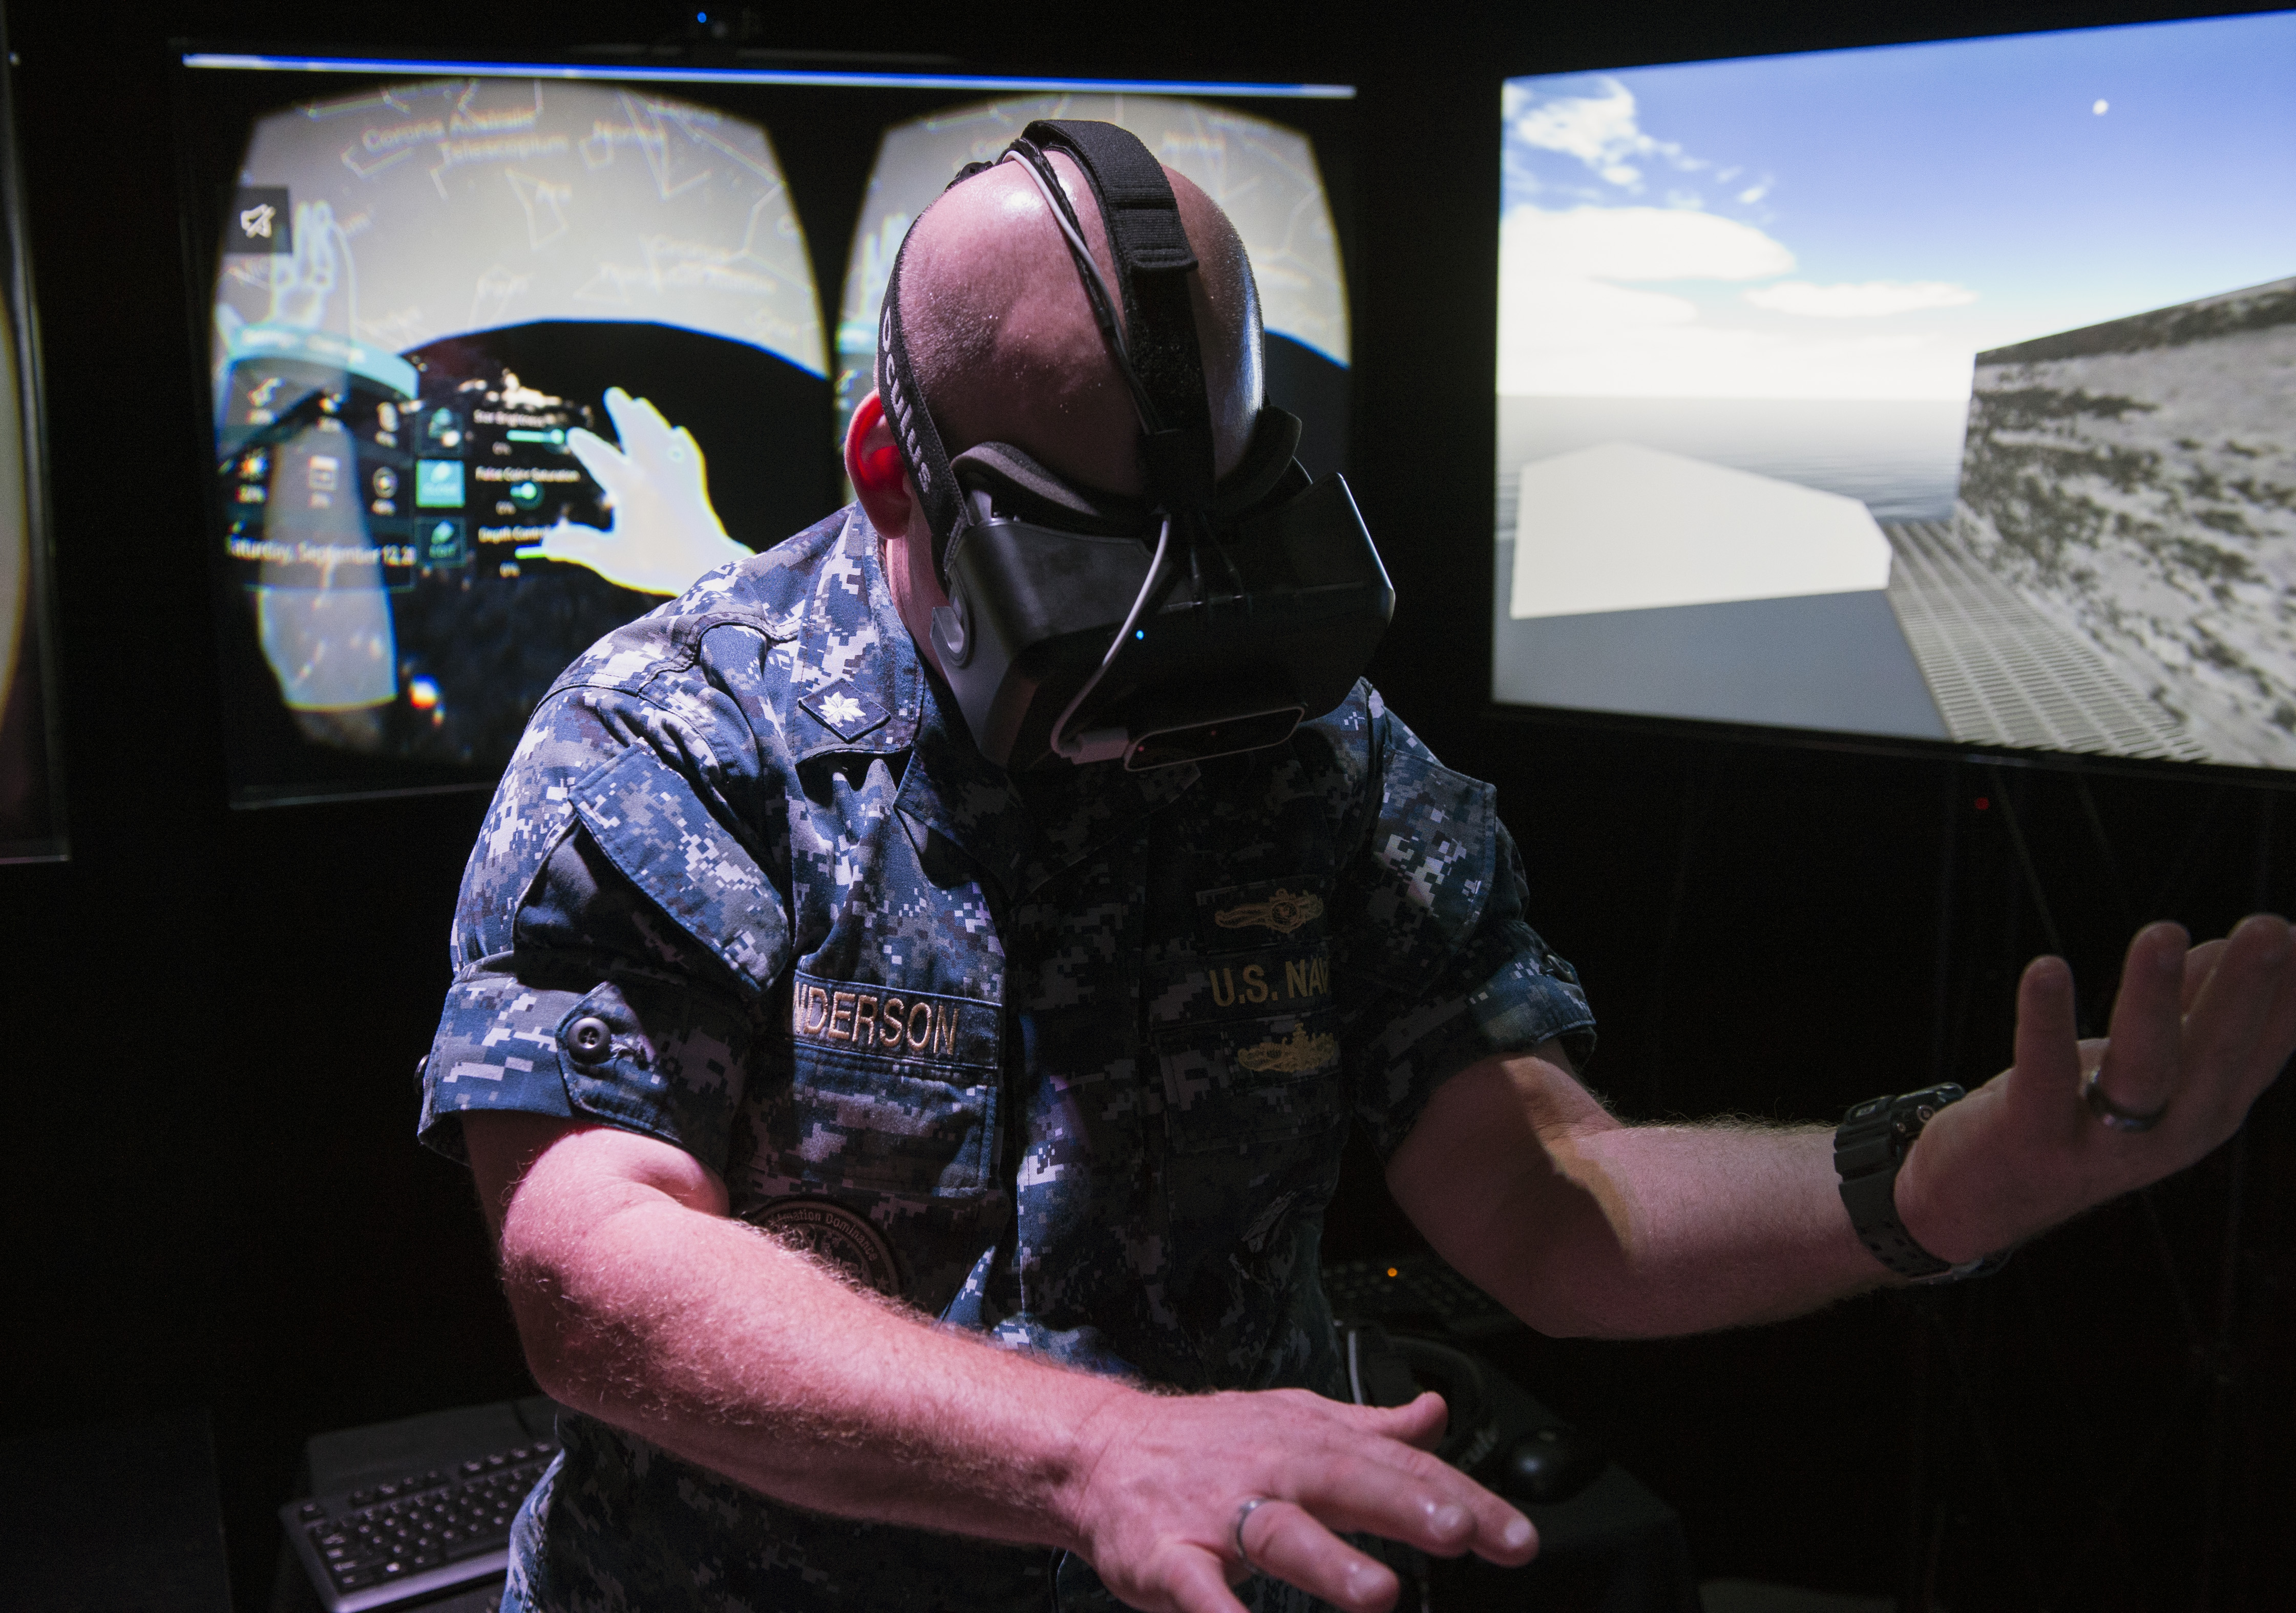
\includegraphics[width=400px]{figs/general/vr_example.jpg}
\caption{An example of the use of Virtual Reality using only hands to interface with the computer\protect\footnotemark.}
\label{fig:intro:htex}
\end{figure}
\footnotetext{CC-BY-2.0 License (\url{https://creativecommons.org/licenses/by/2.0/deed.en})\copyright$\,${\slshape John F. Williams} (title: 150914-N-PO203-142), obtained from \url{https://www.flickr.com/photos/usnavyresearch/23496662185/} (accessed 29th April 2020)}
% The goal of this dissertation is to investigate the current state of synthetic data generation methods for hand tracking systems using the MANO model. This is achieved by comparing the synthetic data with real data: the MSRA dataset\cite{sun2015cascaded}. The comparison is performed by training an existing hand tracking system, the V2V-Posenet model\cite{moon2018v2v}, with both kinds of data, and cross comparing the resultant models.

\section{Motivation}
\label{sec:intro:mot}
In recent years and decades, as computer technology has improved, new possibilities for human-computer interaction have emerged. This ranges from punch cards, to keyboards, to mice, and touch screens. The developments that these innovations have led to need not be enumerated here. Progress has been made in the development of new technologies and ways for human-computer interaction, which is being lead by the emergence of new technologies such as Augmented Reality (AR) and Virtual Reality (VR). While both technologies have been around for some time, one problem with them is how a user interacts with them. The use of human hands offers the potential to improve the human-computer interaction with these technologies, but hand tracking notoriously difficult problem. More recently, as of writing the world is under lockdown due to Covid-19. Computer mice and keyboards, due to the need to touch them are inevitable vectors of disease, and interacting with a computer using hand gestures alone offers a less risky way of using them. 

The specific motivation about using synthetic data to train a hand tracking system in this project is largely influenced by the {\slshape 5th International Workshop on Observing And Understanding Hands in Action} ({\slshape Hands 2019})\footnote{\url{https://sites.google.com/view/hands2019/home} (accessed 29th April 2020)}. The goals of this challenge are discussed more formally in \cite{armagan2020measuring}. The {\slshape Hands 2019} challenge provides three different tasks for: depth-based hand pose estimation, depth-based hand pose estimation with hands interacting with objects, and RGB-based hand pose estimation with hands interacting with objects. In all three of these tasks, participants are encouraged to use the MANO model to train with synthetic data.

\section{Objectives}
The objective of this dissertation is to evaluate the current state of generating synthetic data in 2020 towards improving the performance of hand tracking systems. This is achieved by comparing synthetic data generated with real data: the MSRA dataset \cite{sun2015cascaded}. The comparison is performed by training an existing hand tracking system, the V2V-Posenet model \cite{moon2018v2v}, with both kinds of data, and cross comparing the resultant models using a performance metric. The performance metric is Mean Squared Error (MSE), and is discussed in Section \ref{sec:pm}.



% While there have been previous attempts at generating synthetic datasets for hand tracking systems, this is to my knowledge the first time that a side-by-side comparison has been performed with a real hand tracking dataset to asses its quality.

\section{Overview}
Two synthetic data generation strategies are investigated. The first strategy generates the data based on random parameters for MANO, this is referred to as the {\slshape Random MANO Dataset}. The second strategy generates the data based on parameters determined from the groundtruth of the real dataset to recreate that real dataset using inverse kinematics, this is referred to as the {\slshape IK MANO Dataset}.

The key contributions of this dissertation are 
\begin{enumerate}
    \item Generating a new synthetic dataset using the MANO model.
    \item Performing a side-by-side comparison between a synthetic and real hand tracking dataset using the state-of-the-art synthetic hand data generation method, MANO.
    \item Providing a new framework for generating a synthetic dataset by using a real dataset as a basis.
\end{enumerate}

The rest of this dissertation is divided as follows. Section \ref{chap:lit} discusses and evaluates the previous work around hand tracking systems and datasets. Section \ref{chap:sd} discusses the underlying theory of what synthetic data is, the implications of training a hand tracking system with it, and the strategies used to generate such data. Section \ref{chap:es} discusses the practical details of the experimental setup used for this dissertation. Section \ref{chap:res} presents the results of the experiments to compare the synthetic and real dataset. Section \ref{chap:con} concludes this dissertation.


% Hand tracking systems have become ever more sophisticated \cite{}, however a 

% The key contributions of this dissertation are (1) framing an alternative approach to training a hand tracking system through transfer learning, (2) performing a side-by-side comparison between a synthetic and real hand tracking dataset, and (3) providing a new framework for generating a synthetic dataset by using a real dataset as a basis.

% \section{Hand Tracking}
% What is hand tracking, what are its goals, compare rgb and depth, describe the hollistic pipeline.
% Any background

% \section{Goals}
% Why am I making synthetic data, what are the goals
\chapter{Literature Review}
\label{chap:lit}
% \section{Hand Tracking Systems}
% Latent regression forest: structured estimation of 3d hand poses

% \section{Datasets}

This section will outline the state-of-the-art in hand tracking. Given the nature of this project, a particular focus is put on works that produce datasets for hand tracking, as well as systems that use depth sensors. As well as this, other works investigated include the related problem of full body pose estimation, as well as hand tracking with RGB sensors. The aim in this section is to establish the general idea of what a modern hand tracking system entails, how these systems adapt to the real world, and any relevant gaps and problems in research.

\section{Previous Work}
\subsection{Data}
% \subsubsection{Hand datasets}
A common issue highlighted in literature is a lack of data \cite{armagan2020measuring}, leading many to produce new datasets for training hand tracking systems. There are broadly two kinds of hand tracking datasets. Firstly, depth-based datasets consist of depth images. Such images capture the depth information of the scene. Secondly, RGB-based datasets consist of colour images of the hand. Some systems use both depth and RGB images for hand tracking. Different datasets also employ different labelling regimens. Most datasets aim to annotate the 3D locations of keypoints. These keypoints consist of certain points of interest in the hand, typically the knuckles, wrist, and finger joints. Some datasets only annotate the 2D keypoint locations which is easier to produce, while most datasets discussed here annotate the 3D keypoint locations, as this provides a richer feature space to extract information about the hand, although it is more difficult to estimate 3D keypoints as opposed to 2D keypoints. Another labelling strategy is to segment the images into different parts, such as the region that contains particular fingers. The other distinction between hand tracking datasets is whether they are real or synthetic datasets.

The {\slshape NYU} dataset \cite{tompson2014real}, which is based on depth images is one of the first modern hand-tracking datasets. The authors describe a comprehensive pipeline for acquiring data, and then training a {\slshape convolutional neural network} (CNN) with that data, to produce a system that can infer the continuous pose shape of a hand. In the dataset creation pipeline, the hand is first segmented using a {\slshape randomised decision forest}. Then using an initial approximation of the pose parameters, a {\slshape particle swarm optimisation} algorithm is used whereby a candidate pose is used to generate a synthetic image using an {\slshape linear blend skinning} (LBS) model. The captured image is compared against the generated image using an objective function and the candidate pose is updated using a loss function. The {\slshape Nelder–Mead} method is used to refine the pose estimates. The initial guess of the first frame is manually annotated, and is passed in a chain to each subsequent frame to be labelled. Their dataset is from two subjects, with 72,000 training, and 8,000 test images.

Two new datasets are introduced in \cite{sharp2015accurate}. Their first dataset, {\slshape FingerPaint} consists depth of images of hands whose groundtruth consist of pixel-wise classifications of the fingers of the hand as well as the palm, describing what region of the hand it belongs to, such as the palm, index finger, etc. The ground truth does not describe the location of keypoints. The annotations are generated with the help of an RGB sensor also recording the hand sequence. The hands are `painted' and segmented with a colour segmentation algorithm to generate the labels, with any errors corrected manually. This dataset is not intended for training, instead just for evaluating the performance of a hand tracking system. The other dataset that they generate is called {\slshape Synthetic}, which consists of 1000 synthetic depth images rendered using a 3D mesh model. Unlike {\slshape FingerPaint}, these images are not in a sequence and are in random articulations. Exact details are not available, but it is likely that the groundtruth consists of 3D keypoint positions.

% To be expanded!
Expanding on the labelling strategy of \cite{tompson2014real}, \cite{sun2015cascaded} introduce the {\slshape MSRA} dataset of 76,500 depth images from 9 subjects for evaluating a hand tracking system. Each of the subjects recorded were asked to produce 17 different poses which the authors say are mostly drawn from American Sign Language. The ground truth is generated from another hand tracking system and manually corrected for any errors.

\cite{tang2016latent} introduce a dataset consisting of 180,000 depth images with 3D keypoint annotation. In what they call the {\slshape ICVL} dataset, it contains hand poses from 10 different subjects. Each of the subjects are presented with the same 26 poses to recreate with their hands. They use Intel’s {\slshape Creative Interactive Gesture Camera} to capture the data which they say provides far better depth image quality than previous technologies. The annotation is generated by fitting a point cloud (a series of 3D points which together describe the shape of a 3D surface) version of the depth image to an articulated synthetic hand model. The authors highlight that this annotation system often fails at difficult poses, which means that their dataset largely contains easy frontal poses (where the camera is positioned in front of the subject). To account for this limitation, they compare their dataset with the {\slshape Synthetic} dataset introduced by \cite{sharp2015accurate}.

{\slshape BigHand2.2M} \cite{yuan2017bighand2} is the first large scale hand tracking dataset, containing ~2.2 million annotated depth images of hands for training and evaluating a hand tracking model. They use Intel's {\slshape RealSense SR300}.Sample images can be seen in Figure \ref{figs:lr:bighand}. They highlight the lack of available datasets for hand tracking, and hypothesise the reason is the lack of scalable methods for annotation. They claim existing automatic methods are not accurate enough, or that they compromise the dataset (such as the use of gloves to aid annotation). They say that manual annotation is too slow to make a dataset sufficiently large. They introduce a new capture method for annotation where the hand is fitted with magnets on each fingertip as well as the palm. With a depth camera capturing the data, the annotations are generated using magnetic sensors. They produce 21 3D keypoints using {\slshape inverse kinematics} of the hand to generate the subsequent annotations. Their dataset is from ten subjects.

\begin{figure}
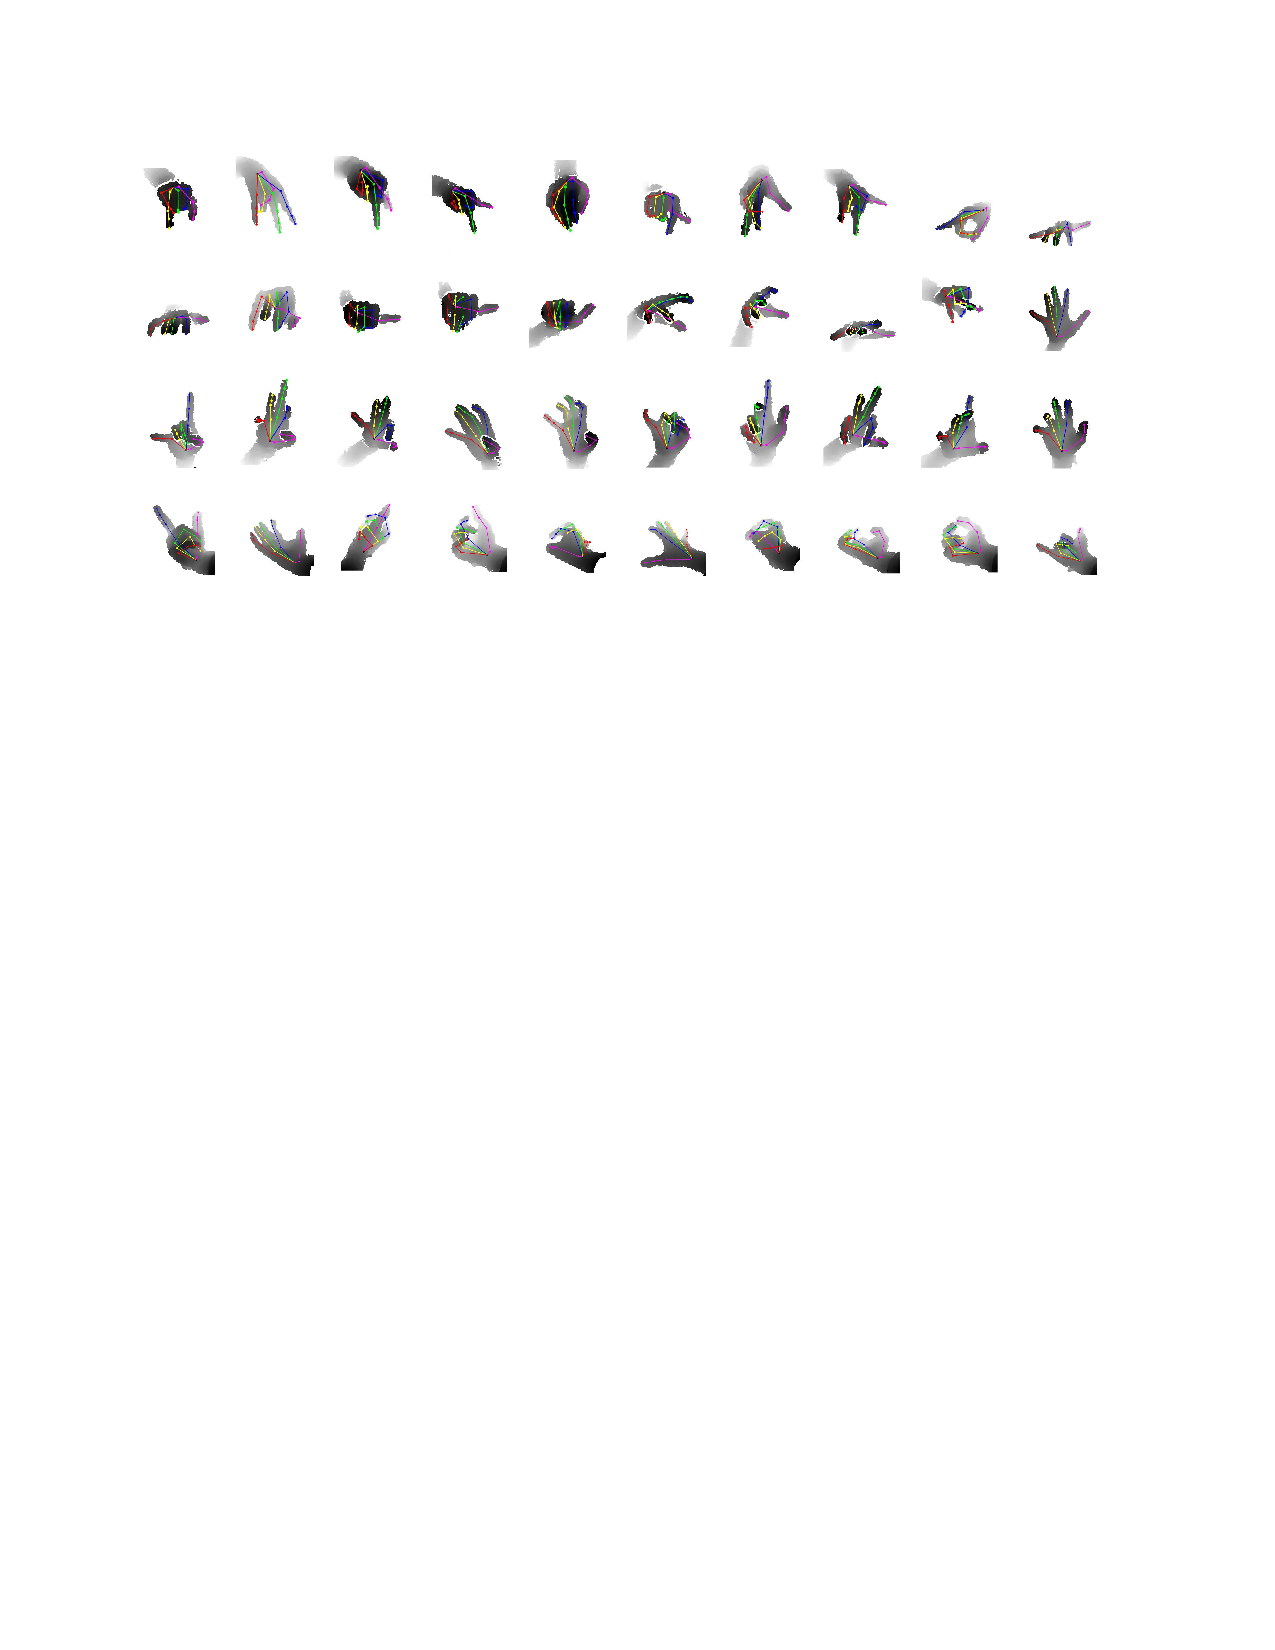
\includegraphics[width=\linewidth]{figs/general/bighand22m.pdf}
\caption{Sample images from the BigHand2.2M dataset with the annotation superimposed. Image taken from the original paper \cite{yuan2017bighand2}.}
\label{figs:lr:bighand}
\end{figure}

\cite{mueller2017real} introduce a new RGB and depth synthetic dataset, {\slshape SynthHands}. They define an egocentric viewpoint as the camera perspective of the hands as is seen from the head or chest. The reasoning behind making such a dataset is that it is challenging to capture the real world annotations of hands, and that existing datasets lack hand-object interactions and realistic hand poses, nor do they show real world noise and backgrounds. They highlight that annotating an egocentric dataset is particularly challenging due to the increased likelihood of self occlusion, which is where the hand blocks part of itself from the camera view. The gestures rendered in the synthetic dataset are generated from real gestures captured from a human hand, with the camera retargeted to an egocentric viewpoint. As well as this, the synthetic hands have artificial interactions with objects, and the background is composited with different scenarios including desktops, offices, corridors, and kitchens.

\cite{malik2018deephps} propose a new dataset, {\slshape SynHand5M}, which contains 5 million synthetically generated depth images of hands in different poses, and camera viewpoints. They claim this approach to be superior to \cite{yuan2017bighand2} and \cite{romero2017embodied}, since they are both based on the data of a small amount of subjects, the nature of their synthetic data generation algorithm means they can vary the shape of a hand, which cannot be done with real data. They also claim that since the data is synthetically generated, the groundtruth is perfect. Their goal in making this dataset is to cover most, if not all possible articulations, shapes, and camera perspectives. To this end, in order to ensure that the hand shapes are realistic, they use limits defined by an anthropometric database. They also set limits to the articulations of the hand. This is because it is easy to deform the synthetic hand into shapes that a real world hand would not be able to achieve, which could lead the hand tracking system that trains on this dataset to learn unrealistic hand articulations. They admit that their specific implementation is not fully realistic, but claim that this is sufficient as a pretraining step for the CNN that they use for their hand-tracking system.

\cite{wang2018mask} highlight the lack of data available for training RGB based systems. They show that existing RGB based datasets are synthetic, or captured in a lab setting. Unlike depth images, RGB images have to have a background to simulate real life use, and the background has to vary too or else the model may just learn that background and it will not be able to segment other types of backgrounds. Their new dataset is called {\slshape OneHand10K} which consists of 11703 RGB images with varying backgrounds, and annotated for 21 2D keypoints. The groundtruth is manually annoted by at least three different people marking, and keypoints that are not visible in the dataset are not annotated.

\subsection{Rendering Methods}
A new full-body statistical model is introduced in \cite{romero2017embodied} called MANO. Built on previous full-body statistical models, MANO is compatible with mainstream computer graphics systems and allows synthetic poses using a set of shape and articulation parameters to model different body shapes and poses seen in real life respectively. MANO places a special emphasis on hands, the authors highlight that recent advances in full-body models have often neglected hands, given their complex articulated nature with respect to the rest of the human body. The model is learned by capturing the full body and hands separately. The hand model data is captured from 31 subjects performing 51 different actions including hand-object interaction. The combined model uses LBS, and the authors say that certain corrective blend shapes are used to mitigate the drawbacks of LBS. The model takes two parameters $\bm{\beta}$ and $\bm{\theta}$ which outputs 778 vertices describing the shape of a hand in 3D space. These vertices can then be put into a standard graphics pipeline for rendering. They use this mesh model to improve the hand rendering performance of the full body model SMPL \cite{loper2015smpl}.

\subsection{Hand Tracking Systems}
A hand tracking system is one that in general, takes a depth, RGB, or both images as an input and outputs a set of 2D or 3D coordinates showing the location of the hand's keypoints. Modern (within the last 3-4 years) systems typically employ some form of CNN architecture, however the basic architectures that have seen success in other tasks such as ordinary image classification are typically not enough and a more sophisticated model is required.

\subsubsection{2D CNN Approaches}
\cite{mueller2017real} approach the problem of hand pose estimation using a combination of RGB and depth cameras from an egocentric perspective as mentioned in the dataset discussion. They combine the RGB and depth images into a coloured depth image (RGBD) first, and from that crop the image to the {\slshape region of interest} (ROI, the part of the image that contains the hand, either a bounding box, or semantic segmention). This is done by passing the image into a CNN which outputs a heatmap. The centre of this heatmap is supposed to be the MCP joint of the middle finger (see Figure \ref{fig:sd:hand} for an illustration). In order to ensure that the location of the centre of the heatmap is temporally consistent, if the confidence of this centre is less than 0.1, and it is more than 30 pixels away from the centre of the previous image, they update the heatmap centre using the sum of the previous frame and the estimate of the current location based on the motion of previous frames that were marked as confident. In a special function, it locates the centre of this heatmap, and using the depth information, it removes pixels that are far away from a 3D Eucliadian perspective. From there, this cropped RGBD image, it is passed into a CNN to regreess the 3D keypoints, as well as a 2D heatmap of these keypoints. The regressed 3D keypoint coordinates are refined using a kinematic hand model, and further refined with the help of the 2D heatmap.

\cite{malik2018deephps} employs a two-stage CNN architecture where given a depth image, they aim to estimate the 3D keypoint locations of the hand, as well as a vertex mesh representing a reconstruction of the hand's surface. Within this CNN, there are three parallel steps for estimating: the hand articulation $\bm{\theta}$, hand shape $\bm{\beta}$ (these parameters are not to be confused with similar notation of MANO), and scale $\alpha$. Inside the same CNN, $\alpha$, $\bm{\beta}$, and $\bm{\theta}$ are then passed into a non-linear differentiable layer (which means that this layer can be trained with backpropagation together with the previous layers) that they call a {\slshape Hand Pose and Shape Layer}. This layer consists of stages to construct a hand representation using the shape parameters $\alpha$, $\bm{\beta}$, and they use the $\bm{\theta}$ then to reconstruct the hand pose using Linear Blend Skinning.

\cite{wang2018mask} approach the hand tracking problem in terms of discovering a set of 2D keypoints in an RGB image. They highlight the advances made in hand tracking using depth sensors and the comparative slowness in progress for RGB systems. Many existing systems rely on strict lighting and backgrounds. Their model is divided into two parts, both are fully-convolutional networks, where the first segments a silhouette (a pixel-wise segmentation of the image into foreground that contains the hand, and background that does not contain the hand), and the second regresses the 2D keypoints. They believe that this approach can be a step towards RGB-based systems for 3D keypoint estimation.

\cite{wan2019dual} address hand tracking in terms of estimating a large set of vertices that describe the surface of a human hand from a depth image. The authors argue that estimating a small set of keypoints is underconstrained, and that estimating the vertices of a hand has more useful applications. To this end, they propose a {\slshape fully convolutional network} (FCN) architecture that estimates these vertices. There are two consecutive hour-glass FCNs. The first FCN has two heads (outputs), one with a generic feature map, and one with estimates 2D mesh coordinates of the image. In a process the authors call {\slshape extension}, the feature map and 2D mesh estimation are combined and passed into another FCN to give an initial estimate of the 3D vertices. This initial estimate is refined using a kinematic model of the hand.

\cite{liu2019feature} introduce a novel feature boosting algorithm for a CNN network for inferring the 3D keypoints of an RGB image of a hand or human body. They introduce a new {\slshape long short-term dependence-aware} (LSTD) module that understands the relationship between different keypoints to boost the feature outputs of a CNN network. For example, the keypoint relationship between two different keypoints in the same finger are highly correlated, but less so with keypoints in other fingers of the same hand. They highlight that many existing pose estimation methods do not factor the relationship between keypoints, or use keypoint relationships to refine the estimate as a post processing stage. Their network can be stacked into multiple blocks to further refine the keypoint estimate. To account for the unreliability of the features generated by a CNN due to occlusions and textures in the RGB input image, they also introduce a {\slshape context consistency gate} to act as a gating mechanism to the LSTD module which analyses the input features in terms of their context with respect to their neighbouring keypoints, and adjusts any irregularities to improve the estimation of the keypoint locations overall. They claim that their results achieve state-of-the-art results on human body estimation datasets.

\subsubsection{3D CNN Approaches}

\cite{moon2018v2v, ge2018real} both propose similar systems where depth image representation of a hand, is inputted to a 3D CNN to predict the 3D keypoints of the hand. The depth image, a 2D pixel array is converted into a 3D voxel (a voxel is the 3D equivalent to 2D pixels) representation and then passed into the CNN for inference. The authors cite the fact that a depth image really conveys 3D information, and they hypothesise that passing in a 2D depth image into a 2D CNN discards the 3D data, leading to reduced performance. \cite{moon2018v2v} discuss this hypothesis by running four experiments; a depth image is used to infer 3D keypoints, a depth image is used to infer voxelised 3D keypoints, a voxelised depth image is used to infer 3D keypoints, and a voxelised depth image is used to infer voxelised 3D keypoints. Their experiments show that a voxelised depth image used to infer voxelised 3D keypoints delivers superior performance over the other methods, they call their new architecture {\slshape V2V-PoseNet}. \cite{ge2018real} investigates this hypothesis by running these four experiments. Firstly a depth image is passed into a CNN to estimate the heatmap for each keypoint location. Second, the voxel representation of the hand is used to generate multiple depth map images from different perspectives and passed into a 2D CNN to estimate a series of heatmaps for keypoints for each input. Third, the single depth image is passed into a CNN to directly estimate the 3D keypoints. Fourth, the voxelised image is passed into a 3D CNN to estimate the 3D keypoint locatioins. \cite{malik2020handvoxnet} takes {\slshape V2V-PoseNet} one step further by also trying to estimate hand shape in addition to pose using more 3D CNN architectures in what they call {\slshape HandVoxNet}.

\begin{figure}
    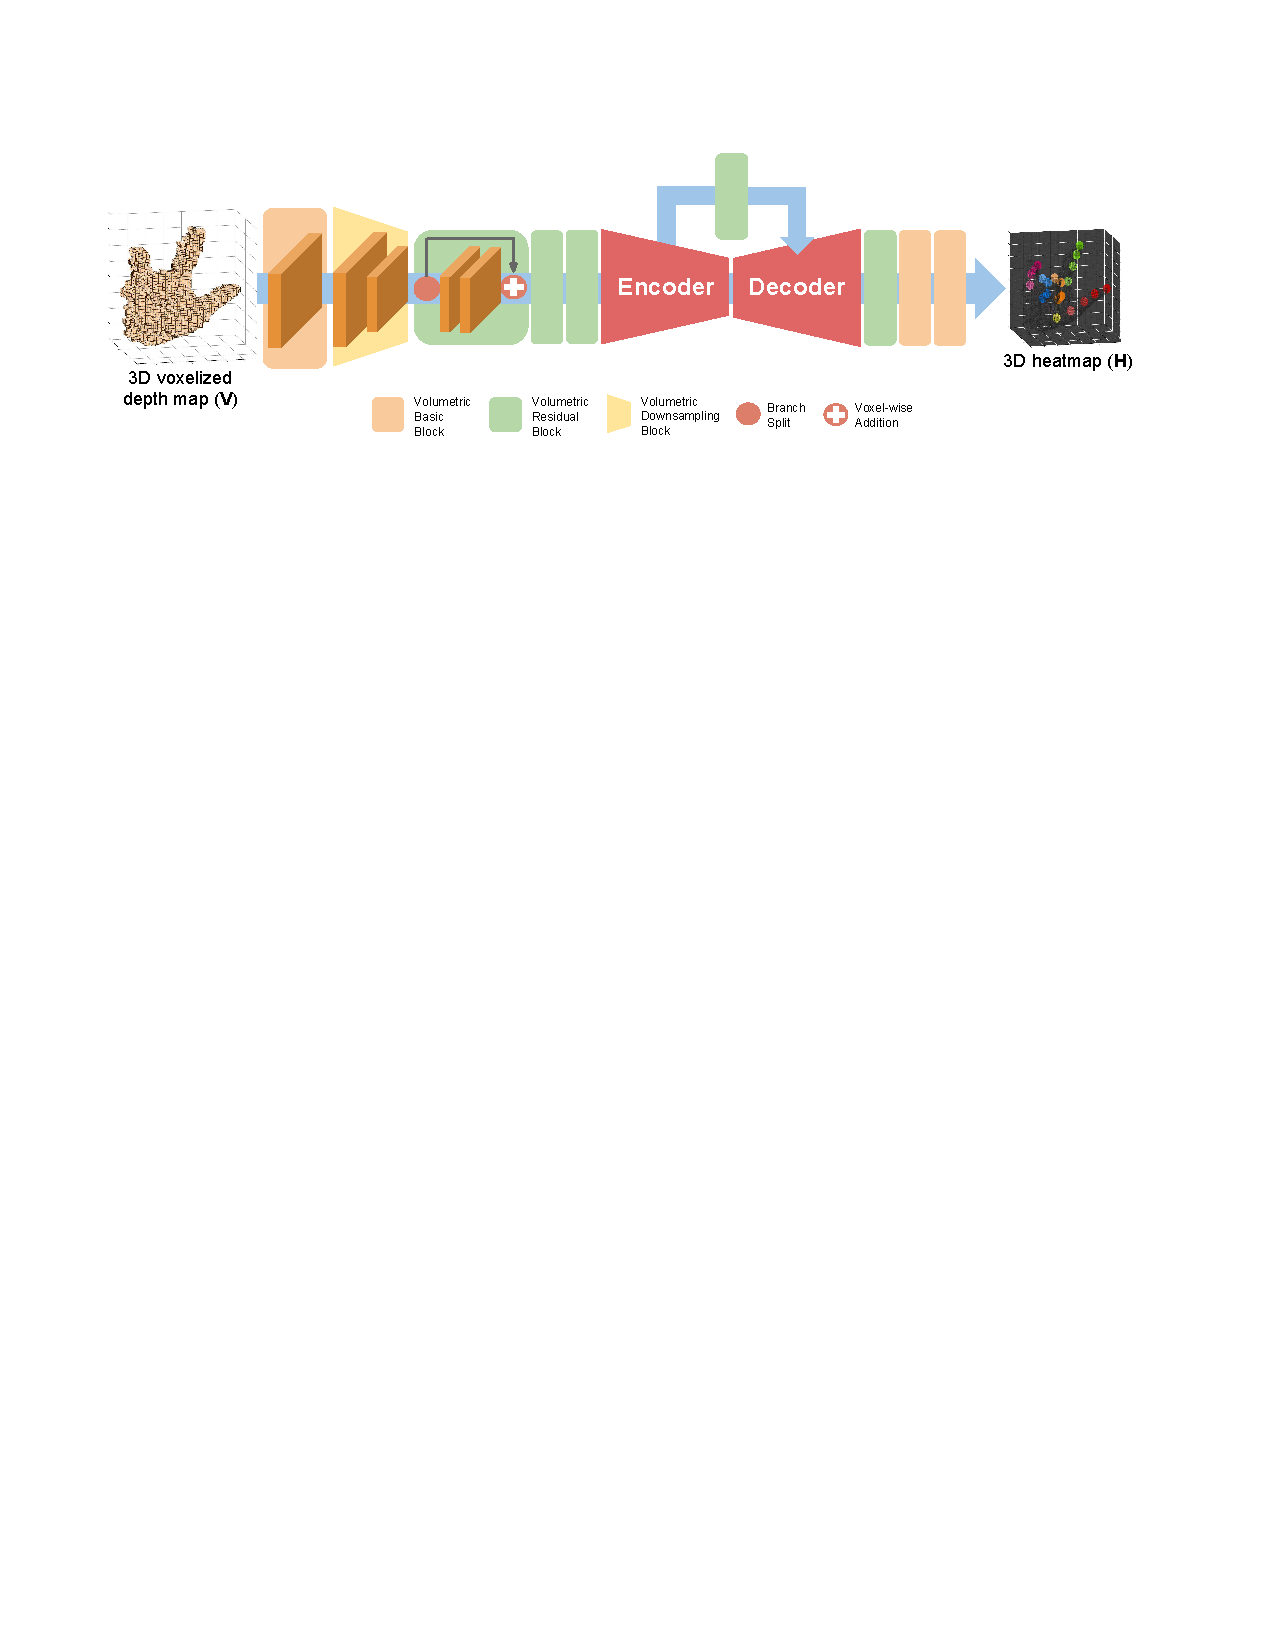
\includegraphics[width=\linewidth]{figs/general/v2v-posenet.pdf}
    \caption{An illustration of the V2V-Posenet model. Image taken from the original paper \cite{moon2018v2v}.}
    \label{fig:v2vposenet}
    \end{figure}

\subsubsection{Generative Approaches}
Generative Adversarial Networks (GANs) are a recent neural network architecture where two components are trained in tandem, a generator to generate synthetic data, and a discriminator to tell whether it is real or not \cite{karras2017progressive}. The idea is that both components engage in a race to outperform the other, and ultimately we get a good system for generating synthetic data, and a good system for telling whether that is real or fake by both networks working against each other.

\cite{he2019graphposegan} address hand tracking for RGB images by adopting this GAN approach. In this paper, the authors use the generator to estimate the hand pose in a two stage process where an initial estimate is generated, and further refined using a parametric hand model. The discriminator acts effectively as a loss function, distinguishing between the predicted keypoints and groundtruth.

\cite{oberweger2019generalized} highlight how many recent works in hand pose estimation rely on a 3D hand model as part of the estimation process. They hypothesise that this is not an ideal approach given that these hand models are simplified and do not take the actual anatomical characteristics of the hand into consideration. Given a depth image as an input, they aim to estimate a set of keypoints describing the hand articulation, which is achieved as follows. After obtaining a box-shaped ROI of the hand, this is passed into a CNN to give an initial estimate of the 3D coordinates, which is passed into another CNN model that generates a synthetic image, in a similar approach to the generator in \cite{he2019graphposegan}. The real and synthetic depth images are passed into another CNN that updates the estimate of the keypoints, which is passed back into the generator CNN again in an iterative process.

\cite{chen2020dggan} propose a simple GAN for RGB-based pose estimation. They highlight the recent advances made in hand pose estimation using depth images, but they believe RGB-based methods to be ultimately superior because RGB sensors are cheaper and more readily available. Combining these two ideas, they aim to train a system that generates a depth image from an input RGB image in one module. In the other module, the 2D keypoints are directly estimated on the RGB image, then the 3D keypoints are regressed from that. This estimate is then refined using the generated depth image. The generative component needs to be trained with paired RGB and depth images, but it can then be trained on RGB images alone after that and they claim that the generative component can improve the estimate versus using RGB alone such as \cite{wang2018mask}.

\subsubsection{Cascaded Regressors}
\cite{sun2015cascaded} highlight recent successes in full body classification algorithms that classify the body into different regions based on what body part that they belong to, but that this approach does not work well for hands. They believe that this is because full body images are easy to classify, they tend to be all frontal-based. Hand images in contrast tend to have more varied camera angles and the hand is capable of deforming in far more diverse orientations. They therefore believe that regressing the pose of the hand, that is estimating the locations of 3D keypoints describing the locations of certain parts of a hand in 3D space is a more principled approach to the problem. They believe however that current regression techniques such as CNNs do not have the capacity to learn all of the possible variations in human hand poses. To address this hypothesis, they believe a cascaded regression approach for hand tracking is superior. Cascaded regression works by using a pipeline of weak regressors. They extend previous work for 2D cascaded hand pose regressors into 3D.

\cite{tang2018opening} address the problem that modern hand tracking systems are typically `black box' systems. That is, that the hand is passed into some model and it outputs the parameters without us knowing what is actually going on inside the system beyond the basic mathematics. This is a general problem within machine learning. They specifically address this issue for {\slshape analysis by synthesis} depth hand tracking systems such as \cite{sharp2015accurate}. In a process that they call {\slshape hierarchical sampling optimisation}, it uses knowledge of the hands structure to estimate the keypoints of the hands in a hierarchal way from the wrist towards the fingertips. Then, like \cite{sharp2015accurate}, this is used to render a synthetic version of the hand and compared against the original depth image using a scoring function.

\cite{yoo2019capturing} propose a hierarchal CNN for estimating the keypoints of a hand from a depth image. They highlight the progress made in accurate hand tracking in terms of reduced error, but also highlight the fact that some of the more accurate systems have a high computational overhead, particularly V2V-Posenet \cite{moon2018v2v}. Their system passes a depth image through an encoder, then the keypoints for the thumb, palm, and each finger are separately estimated in discrete CNN blocks to output 3D keypoints. Their system is more accurate than all of the systems that they survey except for \cite{li2019point, moon2018v2v}, however it is still faster than them.

\subsubsection{Mesh Recovery}
\cite{sharp2015accurate} introduce an {\slshape analysis by synthesis} approach for hand tracking. {\slshape Analysis by synthesis} is an approach to computer vision that uses {\slshape Bayesian inference}. This idea posits traditional machine learning where a model learns from data as `bottom up' processing, and they argue that we can gain more accurate insights about a problem by also considering a `top down' approach \cite{yuille2006vision}. The idea is that given an input image, an attempt is made to reverse the process of how that image was generated. In a simple example of classifying a pattern of text, this method says that we should separate this problem into components such as the probability of the font, noise, overlap, obstruction etc to get towards the core problem, that is: what the actual text is. In terms of hand tracking, this approach works by taking a depth image as an input, first segmenting the ROI. Then, the global rotation and subsequently local articulation are estimated to generate a series of candidate poses which are rendered into synthetic images. This synthetic image can then be compared against the original using a simple pixel-wise MSE function to choose the best one. This initial estimate is then refined using {\slshape particle swarm optimisation} combined with information from previous frames in the same video sequence.

\cite{baek2019pushing} uses the MANO model \cite{romero2017embodied} at the centre of their hand tracking system. Their system aims to predict 778 3D vertices describing a hand shape from an RGB input, in a similar `top down' approach to hand tracking as \cite{sharp2015accurate}. Instead of trying to predict this directly, they have a three-stage pipeline employing CNN architecture to achieve this. The first stage consists of two parts; one CNN generates a 2048-dimensional feature vector of the foreground of the image containing the hand, and another CNN estimates the 21 2D keypoints of the hand. A second CNN takes these features and keypoints as an input and outputs a 63-dimensional vector. The first 45 parameters are the articulation parameters for the MANO model $\bm{\theta}$, the next 10 are the MANO shape parameters $\bm{\beta}$, the next four are the camera rotation in quaternion space, one for scale, and the final three are for the camera translation. As previously described, the MANO model outputs 778 vertices given the articulation and shape parameters. The 778 vertex output can then be rotated, scaled, and translated as appropriate using the rotation, scale, and translation parameters. These 778 vertices are then passed to a regressor to obtain 21 keypoints in 3D space.

\subsection{Related Tracking Systems}

\cite{hoffmann2019learning} looks at the problem of full-body tracking. The authors specifically address the problem of the lack of training data for full-body tracking for RGB-based systems. Using the full-body version of MANO - (SMPL+H) \cite{romero2017embodied}, they produce two datasets, one containing fully-synthetic data, and one that is combined with a real dataset as an effective augmentation strategy. A large emphasis in the paper is trying to generate photo-realistic data, given that this is an RGB-based system. The generation of photorealistic data is not a problem limited to synthetic and is a general problem in computer graphics. One of the important insights about synthetic data from the paper is that some synthetically-generated images can convey more information than others. They use Mask R-CNN for segmentation and an existing model to generate shape parameters. To aid in training with synthetic data, they propose an adversarial approach which they call a `student teacher framework'. In this framework, synthetic images are grouped into ten groups based on camera position and the distance of a person to the camera. In training, a real image that has the highest loss per keypoint in the previous $N$ images is used to determine which type of synthetic image to use for training to ensure the network trains on the most difficult synthetic images.

% , and that only more difficult to train samples to limit the use of synthetic data
% Potentially i

% RAW -->


\section{The Modern Hand Tracking System}
% \begin{figure}
% \centering
% \includegraphics[width=250px]{figs/general/churchill_vsign.jpg}
% \caption{Image obtained from the {\slshape UK War Office Second World War Official Collection}. This illustrates the V sign, and the ambiguity between a polite, and rude gesture that a computer might misclassify. Winston Churchill famously was unaware of the vulgar meaning of the hand gesture.}
% \label{fig:lr:churchill}
% \end{figure}
The goal of hand tracking system is to find and extract information about a hand from an image containing one. That information must be sufficiently accurate to distinguish it from some other meaning. 

% Human hands play an intimate part in human communication, and many cultures have different etiquettes for what certain hand gestures mean. For example, the hand {\slshape V sign} (see Figure \ref{fig:lr:churchill} for an illustration) can convey two very different meanings depending on the global orientation of the hand. The most obvious application of a hand tracking system is for Virtual Reality, and Augmented reality headsets, as highlighted in many of the papers above. It is my opinion however that many new technologies find uses in ways that are hard to predict.

The general idea of modern hand tracking systems is as follows. Given an image (RGB and/or depth) that contains a hand, the image is first segmented to a Region of Interest (ROI) which is either semantically segmented (pixel-wise), or segmented with a tight bounding box. From there, the ROI is passed into a model that employs a neural network and sometimes an additional system to take the shape of a hand into account. From there, the system outputs a series of 3D points that describe the locations of certain  keypoints in the hand. This selection of keypoints can then be used to extract what information the hand is conveying in a low-dimensional environment, examples of this include \cite{devineau2018deep, nguyen2019skeleton, wang2019spfemd}. Most research effort appears to go into the use of depth cameras because the input is often less ambiguous than RGB images, and it preserves spatial information about the hand. This has been encouraged by the increasing popularity and quality of depth sensors. RGB-based hand tracking at this time appears far more elusive, given the increased ambiguity in the image due to diverse backgrounds, different skin colour, lighting, among other ambiguities. To give an example of this difference, it is easy to segment a depth image of a hand in front of a wooden floor by discarding all distant pixel values, in contrast with an RGB image, the skin color might be similar to the wooden floor so the segmentation task is far more challenging.

One issue highlighted in literature is the lack of data, many of these same papers also produce a dataset of their own to address this. Part of the problem is that it is difficult to make such datasets, as well as this, many of these datasets rely on few participants, usually in the order of 10-20 participants at most. The core of many modern hand tracking systems use CNNs, which require large datasets to train on. Exactly how much a hand tracking system needs is unknown, but other CNN tasks require in the order of 100,000-1,000,000 images or more. The reason for the lack of hand tracking data is that labelling it is difficult. It is far too labourious for a human to label a hand dataset at scale, and indeed the accuracy may not be good. Notably in \cite{wang2018mask}, they manually annotate their dataset, but this is only for 2D keypoints, and they simply omit keypoints that are occluded from the image. Other computer vision applications have seen a lot of real-world success because of the existance of large datasets for their domains, notably image classification\footnote{\url{http://image-net.org} (accessed 29th April 2020)}. For image classification tasks, it is far easier to label, notably the {\slshape reCAPTCHA} project got internet users to label images by combining the task with spam detection\footnote{\url{https://www.ted.com/talks/luis_von_ahn_massive_scale_online_collaboration} (accessed 29th April 2020)}. This is not possible with hand tracking however, and no scalable system exists to label a large hand tracking dataset without the help of an automatic method.

To automatically label datasets is a chicken and egg problem. The problem is thus: hand tracking systems need more data, and the data needs to be more accurate, but there is not sufficient data. This data can be captured relatively easily, but to label it at scale is practically impossible, therefore a hand tracking system should be used to annotate the data, but no such system exists. To get around this, past datasets have attached gloves, or other sensors to the hand to find the keypoint locations, but this then compromises the resultant images because the glove or sensor can be seen in the image. More recent examples have used a kinematic model of a hand to refine the estimate of the hand such as in the NYU dataset \cite{tompson2014real}. Other labelling efforts have involves placing discrete magnetic sensors on the fingertips and using an inverse kinematic model to estimate the other points\cite{yuan2017bighand2}. One problem with both of these datasets is that they both have a small amount of participants (two and ten respectively). This problem can be solved relatively easily. A problem that is harder to address however is the quality of the annotation, which goes back to the chicken and egg problem highlighted above. We can only hope that the annotation strategies of \cite{tompson2014real, yuan2017bighand2} are accurate. It is doubtful that the authors manually scrutinised each and every image. This is a big problem, because for any machine learning task, the system will only perform as well as the training data given to it. One way around this is to use synthetic data. This idea is explored in \cite{malik2018deephps}, when they create their {\slshape SynHand5M} dataset with perfect groundtruth, but they used a different hand model which they themselves admitted had limited realism. They also designed a new hand tracking system at the same time,  which means that their dataset has not been validated independently. Progress has been made since then with the advent of the MANO model\cite{romero2017embodied}. They specifically set out to address the problem of a lack of realism with hand data, and to the best of my knowledge, no further attempt at creating a large depth dataset has been attempted since {\slshape SynHand5M}.

These same problems are discussed by \cite{armagan2020measuring}, and they posit MANO as a synthetic data generation strategy to address these problems with existing hand data. As discussed in Section \ref{sec:intro:mot}, the research question of this project is particularly influenced by the {\slshape Hands 2019} challenge. Given these problems, this dissertation explores the most recent synthetic hand data generation technique, the MANO model to see how it can address them.

% To get around the problem of a lack of data, some methods use a hand model in the hand tracking system to refine the initial estimate in an iterative approach by fitting an input depth image against a rendered depth image based on the output of the estimated keypoints \cite{sharp2015accurate}. Other methods try to generate hand data synthetically \cite{mueller2017real,malik2018deephps,hoffmann2019learning}.
\chapter{Synthetic Data}
\label{chap:sd}

Modern hand tracking systems typically employ machine learning, and the type of machine learning model usually used is a CNN \cite{mueller2017real, malik2018deephps, wang2018mask, wan2019dual, moon2018v2v}. Machine learning offers a way to solve a particular task without being explicitly programmed to perform that task. Instead, Machine Learning `learns' how to do this task by `training' on the data. This learned task is further tested on another dataset that the model did not train on to see how it performs. This idea of having a training dataset and a testing dataset is achieved in different ways. For example, in {\slshape k-fold cross validation}, $\frac{1}{k}$ of the dataset is used for testing and the remainder for training. The model is trained $k$ times with a different section of the dataset used for training and testing each time. This method is useful for evaluating the performance of a model. For the purposes of this dissertation, a simpler method of: splitting the dataset into one training and test dataset, so the model is only trained once with the training set before evaluating performance on the test set.

Synthetic data is any kind of data that is not obtained through direct empirical observation. In the context of hand tracking, real data is obtained by a camera, while synthetic data is obtained typically through graphics rendering. Ideally, any machine learning system will be trained with the same kind of data that it is going to be used for future inference, and so synthetic data should aim to replicate what a real-world camera might see as opposed to a perfect image. There are different ways in which training data is made, depending on what kind of pipeline is being used for hand tracking, but this dissertation will follow the patterns used by \cite{yuan2017bighand2, sun2015cascaded}. That is, the synthetic data that is generated consists of $K$ images and associated groundtruths (the annotation of the keypoints) describing the location of $N$ keypoints in 3D space for each image. Each depthmap image $\bm{Z}$ is an $n\times m$ matrix, where $\mathbb{Z}_{n,m} \in \mathbb{N}$ represents an individual pixel in the image, each pixel represents the depth to the nearest visible point, thus it is called a depthmap. A keypoint is a particular location of interest in the hand, such as a knuckle. An illustration of the keypoints used in this dissertation is shown in Figure \ref{fig:sd:hand}. The goal of a hand tracking system is to take $\bm{Z}$ as an input and predict $N$ 3D keypoints $\bm{\Phi}$, where $\bm{\Phi}=\{\bm{\Phi_1}, \bm{\Phi_2}, ..., \bm{\Phi_N}\}, \bm\Phi_{n} \in \mathbb{R}^{3}$. The groundtruth $\bm{Y}^i$, (where $\bm{Y}^i_n\in \bm{\Phi}$) represents the locations of $N$ keypoints in 3D Cartesian space for $K$ depthmap images in a dataset $\bm{\mathrm{D}}$, where $\bm{\mathrm{D}}_k\in\bm{Z}$. The hand tracking system is trained with a training dataset $\bm{\mathrm{D}}^t$, and is tested with a separate test dataset $\bm{\mathrm{D}}^v$. When testing the hand tracking model, the set of predictions $\bm{Y}^o$ (where $\bm{Y}^o_n\in \bm{\Phi}$) is compared with the groundtruth $\bm{Y}^i$. This comparison is performed using a performance metric $E$.

The goal of this dissertation is to train a hand tracking system on synthetic data such that it can accurately predict future keypoints from a real world sensor. The quality of the synthetic data is evaluated by training an existing hand tracking model V2V-Posenet\cite{moon2018v2v} and evaluating its performance with the synthetic dataset in comparison to a real dataset, the MSRA dataset\cite{sun2015cascaded}. To obtain a fair evaluation, the model is not modified. An assumption is made that the right and left hand are the same, all generation of a hand focusses on the right hand in this dissertation, and that the left hand can be obtained by flipping the image on the $y$-axis. The methods used to generate the synthetic data are described herein.

\section{Synthetic Data Generation Methods}
\label{sec:sdgm}
The spread, or domain of data, describes the nature of the data. In the context of hand data, this implies what kinds of hand articulations, hand shapes, and camera angles the data covers. Previous work has generally focussed on `frontal' views, where the camera is facing towards the person. The other main type of perspective for hands is the `egocentric' perspective, where the camera is facing away from the person towards the hand, an example of this is a head-mounted camera looking at the hands. Egocentric perspectives are typically harder for a hand tracking system to recognise because the possibility of self-occlusion is greater.

The MANO model is used as the model for generating synthetic data. In theory, it is possible to generate a comprehensive dataset covering all possible hand articulations, shapes, and camera positions. This is problematic in practice however for several reasons. Firstly, the question of what constitutes a comprehensive dataset is unknown, and given the dimensionality of the problem, the generation of an ever-increasingly comprehensive dataset becomes computationally infeasible for the hardware available in this dissertation (the generation method described in Section \ref{sec:sd:d} takes 607 milliseconds on average to generate a single image). The subsections herein describe two ways of generating synthetic hand data, and they both highlight the dimensionality issue. The first method sees all generation parameters determined at random, which gives a completely random dataset described in Section \ref{sec:rgm}. The other generation method attempts to recreate a real dataset using the groundtruth of that real dataset as a reference.

\subsection{Random Generation Method - {\slshape Random MANO Dataset}}
\label{sec:rgm}
\begin{figure}
    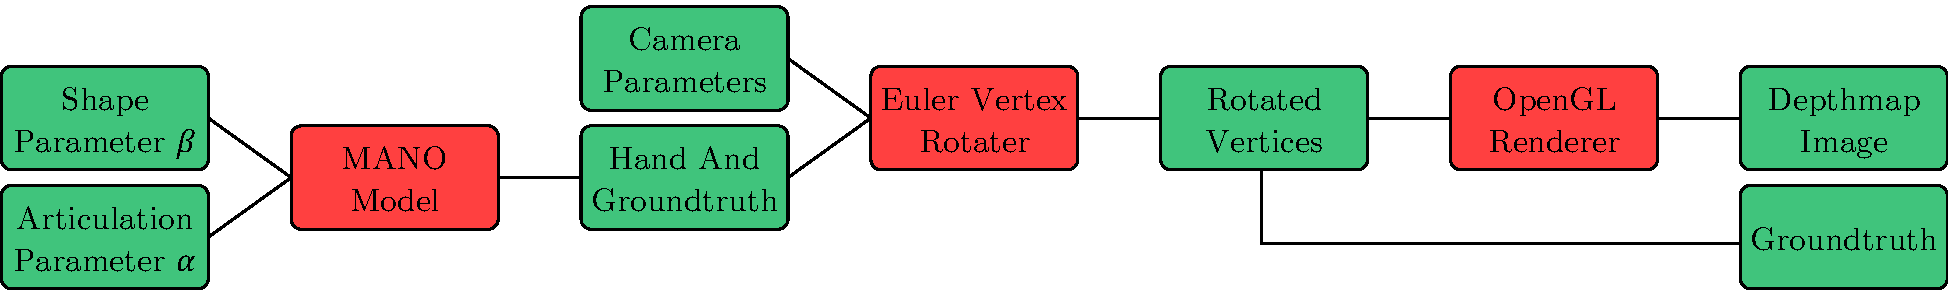
\includegraphics[width=\linewidth]{figs/general/nd_process.pdf}
    \caption{A diagram of the process for generating the Random MANO Dataset. The parameters $\alpha$, $\beta$, and camera parameters are inputs, and the depthmap image and grountruth are outputs.}
    \label{fig:ndproc}
\end{figure}
This is the first synthetic data generation strategy investigated, this dataset is called the {\slshape Random MANO Dataset}. This method involves generating an entirely random synthetic dataset, drawn from a uniform distribution, the meaning of which is described below. A diagram of this process is shown in Figure \ref{fig:ndproc}.
\subsubsection{Generating Poses and Hand Shapes}
The basic MANO model takes two parameters, $\bm{\beta} \in \mathbb{R}^{10}$ and $\bm{\theta} \in \mathbb{R}^{45}$, describing shape and articulation respectively, giving a total of 55 parameters. Following on from \cite{baek2019pushing}, The full 45-dimensional $\bm{\theta}$ parameter is used as opposed to the {\slshape principal component analysis}-based 6-dimensional subspace used in the original MANO implementation. This generates 778 vertices describing a hand based on the input parameters. The groundtruth can be obtained from an additional regressor that takes the 778 vertices as an input and outputs 16 keypoints as a grountruth. I am not aware of any a priori relationship between the input and output of this model, that is, knowing what $\bm{\beta}$ and $\bm{\theta}$ input produces a particular 778 vertex output. Given the size of the input parameters, a random number is drawn for each point $\bm{\beta}$ and $\bm{\theta}$, drawn from a uniform distribution in the range $[-2.0, 2.0]$, the range of values in-between is limited by floating point hardware alone. The underlying theory behind using this regimen is that, given a sufficient number of random draw of values for $\bm{\beta}$ and $\bm{\theta}$, they will eventually converge towards a `comprehensive' dataset insofar as the MANO model can accommodate. Giving the MANO model a zero vector for $\bm{\beta}$ and $\bm{\theta}$ returns a hand in its rest pose (the pose that the hand naturally regresses to when no muscular force is imparted on the fingers), and the greater each index in these vectors deviates from zero, the more diverse of a shape that is outputted (with fingers going in progressively more complex articulations for larger values for each index of $\bm{\beta}$ and $\bm{\theta}$). This particular range was chosen through empirical observation, a range greater than this tends to give unrealistic or impossible poses that a real hand can produce. The original MANO model keypoint regressor outputs 16 keypoints, which does not match with the 21 keypoints used with the MSRA dataset, so in this dissertation, the MANO setup for this project is taken from the code of \cite{baek2019pushing, zhang2019end}.

\subsubsection{Camera}
Before rendering the 778 vertices into a depthmap image, the camera must be set appropriately. The MANO model always generates the 778 hand vertices and 21 keypoints in the same global orientation, therefore they must be rotated afterwards to augment the dataset for different camera perspectives. The image is rendered using OpenGL, and in OpenGL, the camera is always at the zero vector $\bm{0}$ position in Cartesian space, facing in the negative $z$ direction. To manipulate the camera therefore, all of the other vertices in the scene are manipulated, and they must eventually be in the space between $[-1.0, 1.0]$ for each Cartesian axis to appear in the render\footnote{\url{https://www.khronos.org/opengl/wiki/Viewing_and_Transformations} (accessed 29th April 2020)}.

This version of the model does not include a human body, so the camera must not view the hand in any form of ego-centric perspective because the wrist is cut off from the rest of the body and a hole will be seen in the rendered hand's wrist. The groundtruth describes not only the articulation of the hand, but also the orientation and position of the hand in 3D space. To account for this, any rotation of the 778 vertices must also be performed on the 21 keypoint groundtruth. The rotations are performed using three Euler rotations in practice. Specifically, all over a uniform distribution (in radians), the $x$-axis is rotated in the range $[0, 2\pi]$ radians, the $y$-axis is rotated randomly over $[-\frac{2}{3}\pi, -\frac{1}{3}\pi]$ radians, and the $z$-axis is rotated randomly over $[\frac{2}{3}\pi, \frac{1}{3}\pi]$ radians. The 778 vertices are rendered into a depthmap $\bm{Z}$. Example images generated can be seen in Figure \ref{fig:sd:nd}.

\subsubsection{Normalisation}
\label{sec:sd:nd:norm}
The mean and variance of the rendered image need to be adjusted to match the MSRA images. The variance is scaled to the same as the average variance of the MSRA dataset, and the mean is the same as the mean value of the $z$ coordinate of each groundtruth value.

\begin{figure}
    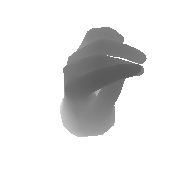
\includegraphics[width=110px]{figs/mano/0.png}
    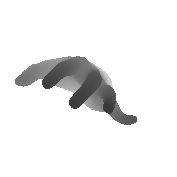
\includegraphics[width=110px]{figs/mano/1.png}
    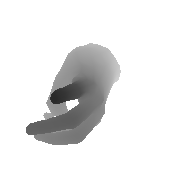
\includegraphics[width=110px]{figs/mano/2.png}
    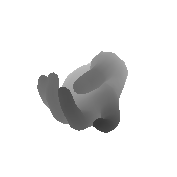
\includegraphics[width=110px]{figs/mano/3.png}
    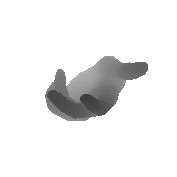
\includegraphics[width=110px]{figs/mano/4.png}
    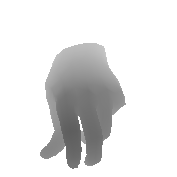
\includegraphics[width=110px]{figs/mano/5.png}
    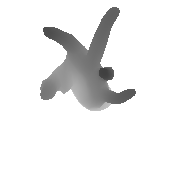
\includegraphics[width=110px]{figs/mano/6.png}
    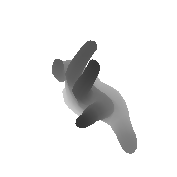
\includegraphics[width=110px]{figs/mano/7.png}
    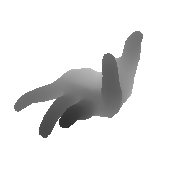
\includegraphics[width=110px]{figs/mano/8.png}
    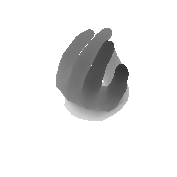
\includegraphics[width=110px]{figs/mano/9.png}
    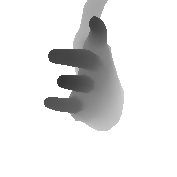
\includegraphics[width=110px]{figs/mano/10.png}
    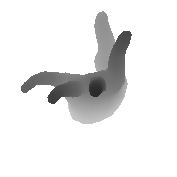
\includegraphics[width=110px]{figs/mano/11.png}
    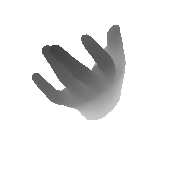
\includegraphics[width=110px]{figs/mano/12.png}
    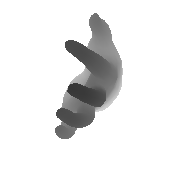
\includegraphics[width=110px]{figs/mano/13.png}
    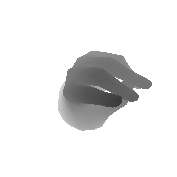
\includegraphics[width=110px]{figs/mano/14.png}
    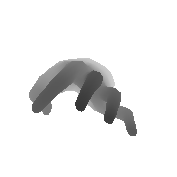
\includegraphics[width=110px]{figs/mano/15.png}
    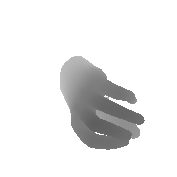
\includegraphics[width=110px]{figs/mano/16.png}
    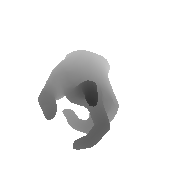
\includegraphics[width=110px]{figs/mano/17.png}
    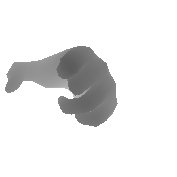
\includegraphics[width=110px]{figs/mano/18.png}
    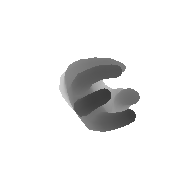
\includegraphics[width=110px]{figs/mano/19.png}
    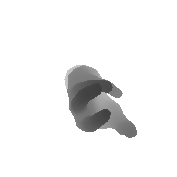
\includegraphics[width=110px]{figs/mano/20.png}
    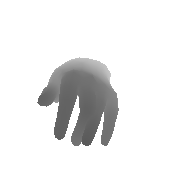
\includegraphics[width=110px]{figs/mano/21.png}
    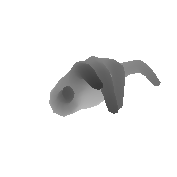
\includegraphics[width=110px]{figs/mano/22.png}
    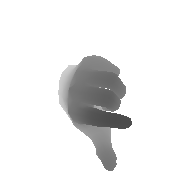
\includegraphics[width=110px]{figs/mano/23.png}
\caption{Examples of images generated using the random generation method.}
\label{fig:sd:nd}
\end{figure}

\subsection{Recreating A Real Dataset - {\slshape IK MANO Dataset}}
\begin{figure}
    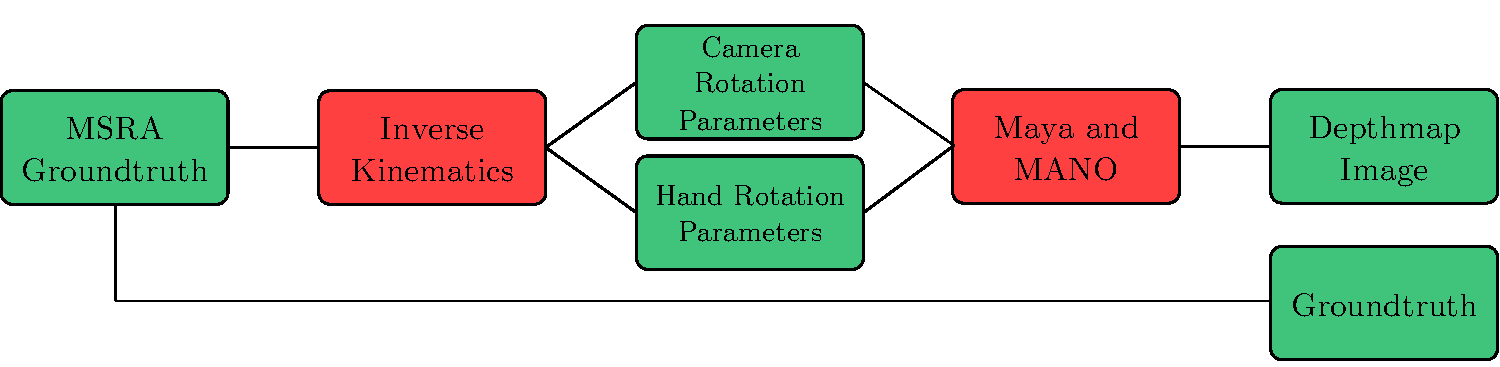
\includegraphics[width=\linewidth]{figs/general/d_process.pdf}
    \caption{A diagram of the process for producing the IK MANO Dataset. Since the recreated depth image should have the same groundtruth as the equivalent MSRA, no processing is performed on it.}
    \label{fig:dproc}
\end{figure}
\label{sec:rard}
\label{sec:sd:d}
\begin{figure}
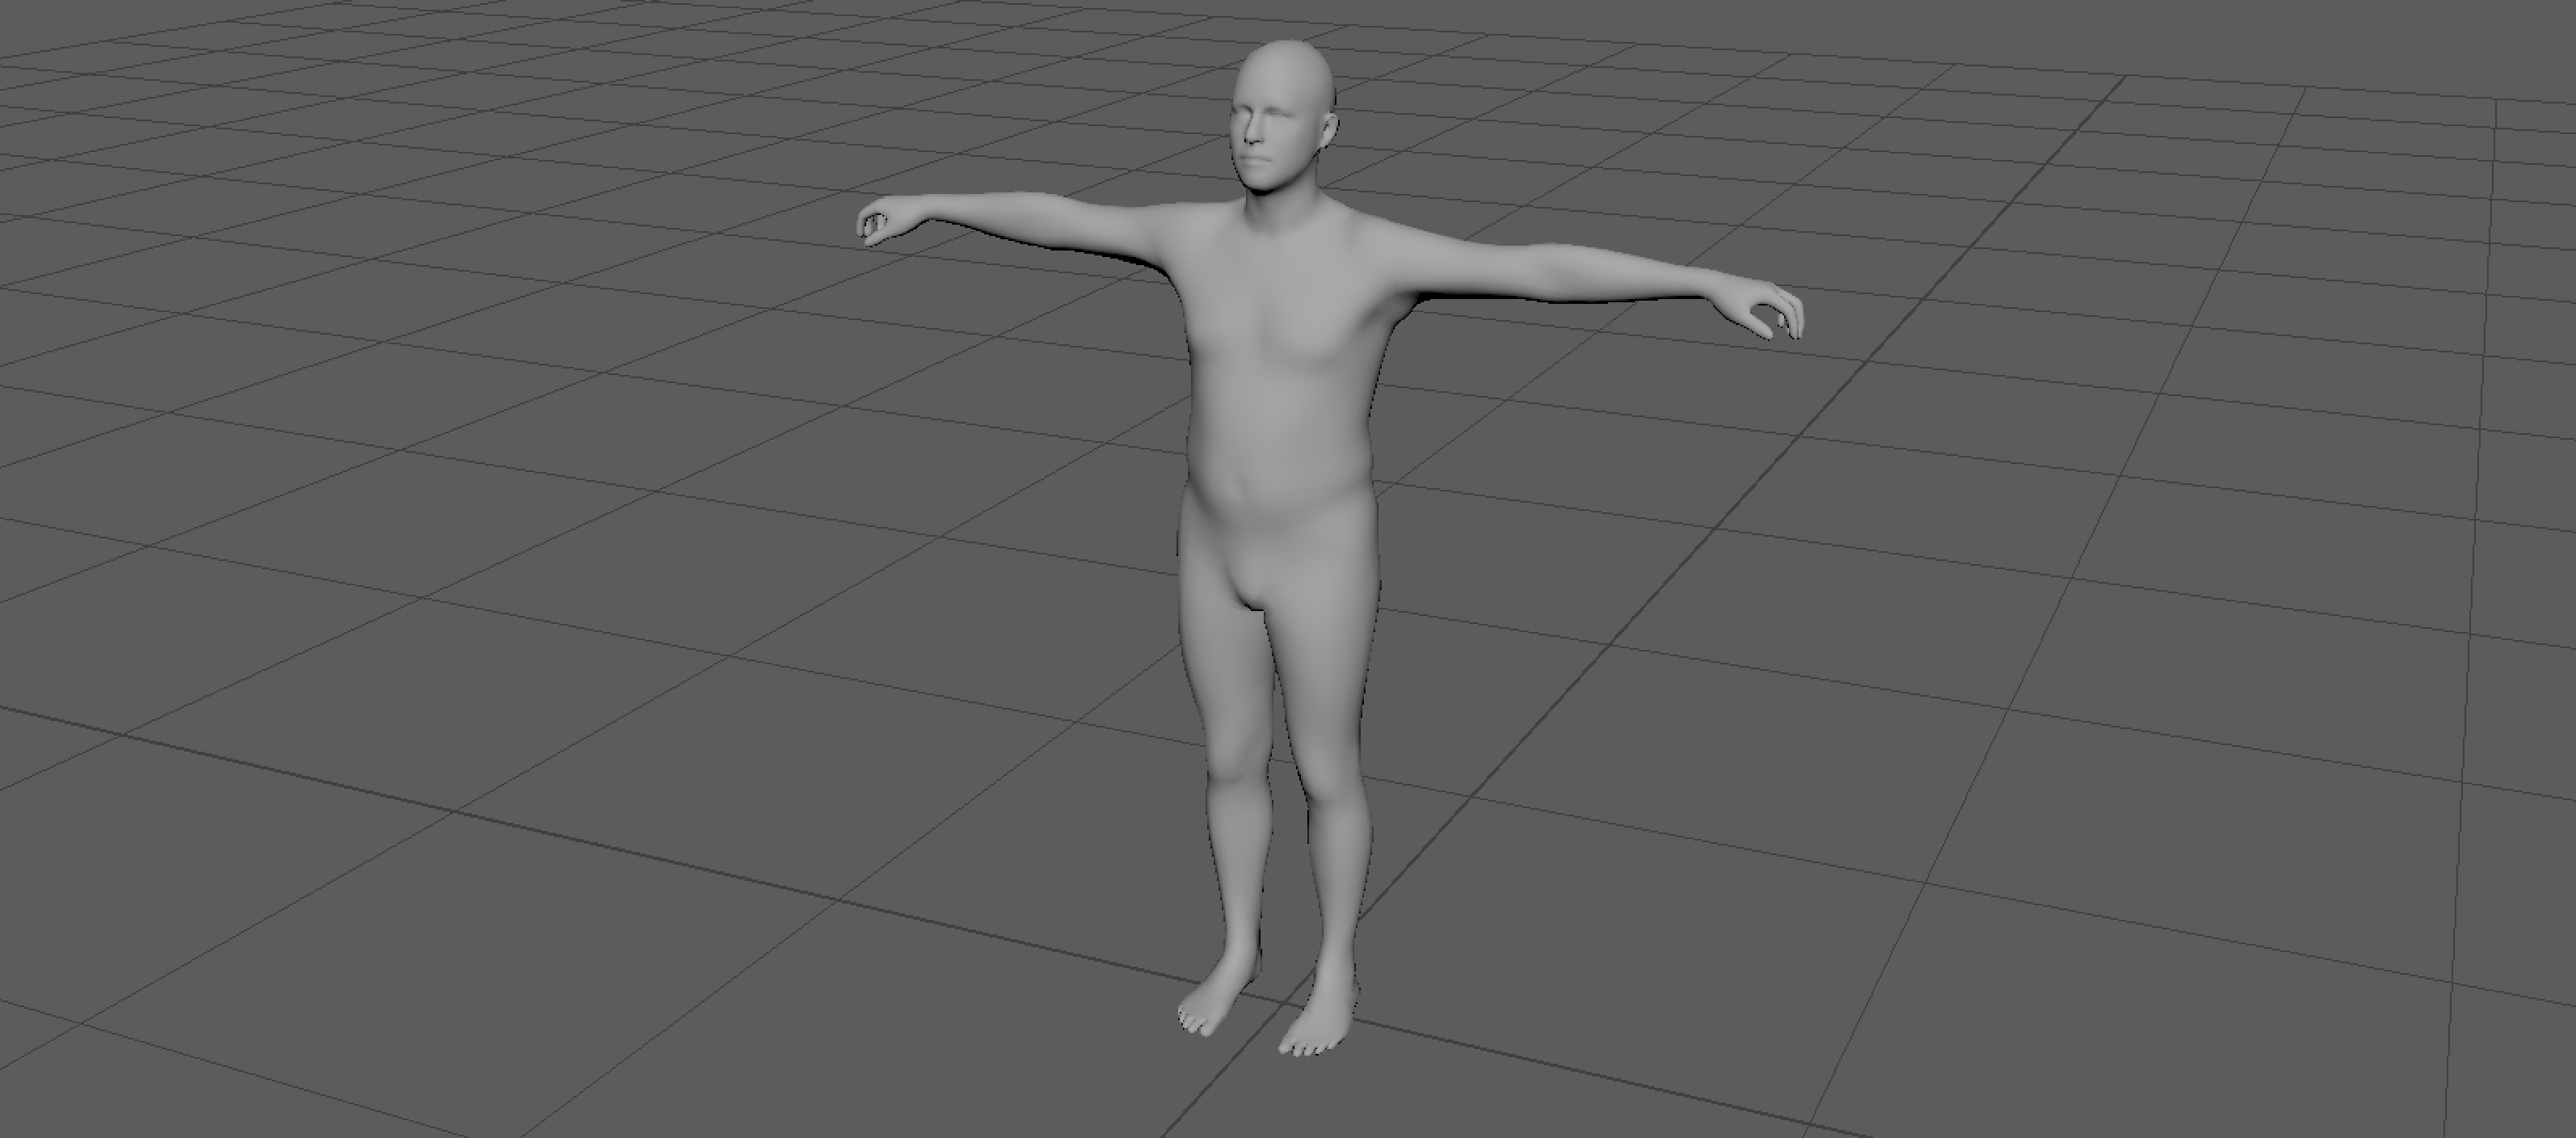
\includegraphics[width=\linewidth]{figs/general/maya.png}
\caption{Screenshot of Maya with the full body MANO model, also called SMPLH.}
\label{fig:smplh_maya}
\end{figure}

This is the second synthetic data generation strategy investigated, this dataset is called the {\slshape IK MANO Dataset}. The random data generation method described in Section \ref{sec:rgm} produces a good dataset in terms of image realism and groundtruth reliability, but it is difficult to compare with the MSRA dataset. As a reminder, the MSRA dataset \cite{sun2015cascaded} is based on certain poses within American Sign Language, and the distribution of poses likely does not match the distribution of data from the random data generation method. To address this concern, this section describes an alternative method of generating synthetic data. The goal of this method is to replicate the MSRA dataset image for image, which offers a direct way of comparing the datasets. This is a similar strategy to \cite{mueller2017real}, where they generated their synthetic data based on the hand pose estimated from a hand captured with a real sensor. To achieve this, the MANO model can be loaded into Maya (as an FBX\footnote{\url{https://www.autodesk.com/products/fbx/overview} (accessed 29th April 2020)} file) as the full human body version (specifically the male version), see Figure \ref{fig:smplh_maya}. In this setup, the hand has 16 keypoints, one for the wrist, and an MCP, PIP, and DIP joint (see Figure \ref{fig:sd:hand}), and each of these joints have three Euler rotation parameters. As well as this, each of these joints have translation parameters which can be used to change the shape of the hand, however this aspect is outside the scope of this dissertation. For hand articulation alone, this gives 45 rotation parameters, which is grossly overconstrained, since it allows us to deform the hand in ways that are not possible for a human. As mentioned in \cite{malik2018deephps}, having implausible hand images might not necessarily be detrimental towards a hand tracking system, however since the purpose of this is to recreate a dataset, this is not be a problem regardless. The following paragraphcs describes the process for reverse engineering the MSRA groundtruth for the purposes of deforming the hand articulation, and how the camera is adjusted to recreate the same camera perspective as the MSRA dataset.

\subsubsection{Extracting hand articulation information from MSRA groundtruth}
\label{sec:sd:d:ex}
There is not a simple mapping from 21 keypoints to 15 finger joint rotations, therefore a mapping needs to be determined to find rotations of the finger to manipulate the MANO model in Maya. Formally, this process is Inverse Kinematics, a subset of Robotics. Human hands though are different to robots since the bone lengths of the MANO model and annotations are different. Taking advantage of the fact that the MSRA dataset includes an annotation for the tip of the finger, the property of the dot product ($\bm{a}\cdot\bm{b}=||\bm{a}||\,||\bm{b}||\cos{\alpha}$) is used to convert the 21 MSRA joint annotation to 15 finger rotations, in a similar way to how rotations are calculated in the {\slshape Cyclic Coordinate Descent Method}\cite{fedor2003application}. These rotations are then used to deform the hand model within Maya. Two joint vectors are subtracted from each other to produce a `phalanx vector' describing the vector orientation between the two joints in consideration, this is described in Equation \ref{eq:dotproduct}. To assist in mapping equation \ref{eq:dotproduct} to the finger rotations in Maya, it is used under the following assumption:

\begin{enumerate}
    \item The palm of the hand (the region between the MCP joints and the wrist) is a rigid body.
    \item All MCP joints have two degrees of freedom - $x$-axis and $y$-axis.
    \item All PIP and DIP joints have one degree of freedom - $x$-axis only.
    \item The four finger MCP joints form a perfectly straight line in 3D space
\end{enumerate}

For simplicity, the wrist is also considered to be a joint. Figure \ref{fig:sd:ikvis} provides an illustration of this process, for example, the vectors $\bm{\Phi}_a$, $\bm{\Phi}_b$, and $\bm{\Phi}_c$ could represent the 3D locations of the MCP, PIP, and DIP respectively for the index finger, and the angle formed by Equation \ref{eq:dotproduct} is the angle that the index finger is deformed at the index PIP joint in the $x$-axis. An enumerated list of rotations performed in the $x$-axis can be found in Table \ref{tb:xrots}.

As stated above, the MCP joint is also assumed to rotate in the $y$-axis, those rotations are calculated as follows. For the pinky finger, index finger, and thumb, their respective PIP and MCP joints are used in conjunction with the next MCP joint. For the middle and ring fingers, this is used for MCP joints on either side, and whichever adjoining combination produces a larger angle in absolute terms is used. See Table \ref{tb:yrots} for a fuller explanation.

\begin{figure}
    \centering
    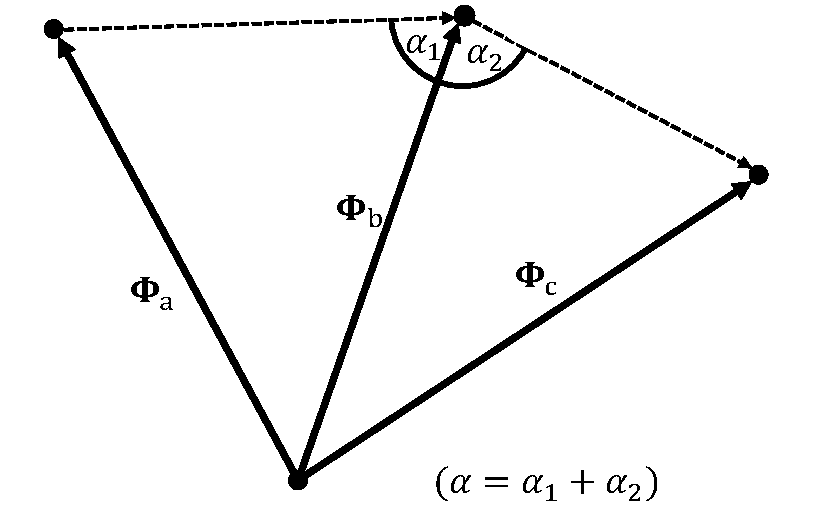
\includegraphics[width=8cm]{figs/general/ik.pdf}
    \caption{A visualisation of how the rotation of a joint is found. $\bm{\Phi}_a$, $\bm{\Phi}_b$, and $\bm{\Phi}_c$ are passed to Equation \ref{eq:dotproduct} to find the angle $\alpha$.}
    \label{fig:sd:ikvis}
\end{figure}

\begin{equation}
    \alpha = \arccos\Bigg({\frac{(\bm{\Phi}_c - \bm{\Phi}_b) \cdot (\bm{\Phi}_b - \bm{\Phi}_a)}{||\bm{\Phi}_c - \bm{\Phi}_b||\,\, ||\bm{\Phi}_b - \bm{\Phi}_a||}}\Bigg)
    \label{eq:dotproduct}
\end{equation}

% \chapter{Enumerated List of Rotations}

% \FloatBarrier\section{}
% \label{sec:ap:enumrotations}
\begin{table}[!ht]
    \centering
    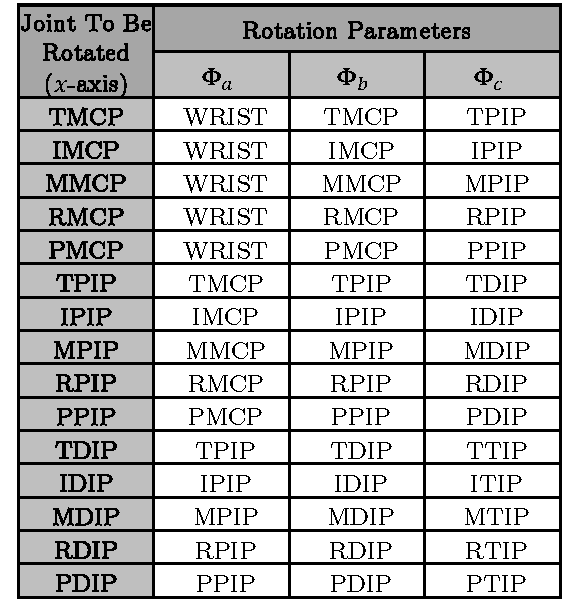
\includegraphics{figs/general/x_rots.pdf}
    \caption{Fully enumerated list of how each joint was rotated in the \underline{{\bfseries $\bm{x}$-axis}} for the inverse kinematics algorithm. See Equation \ref{eq:dotproduct} in Section \ref{sec:sd:d:ex}. See Figure \ref{fig:sd:hand} for details on the joint names.}
    \label{tb:xrots}
\end{table}

\begin{table}[]
    \centering
    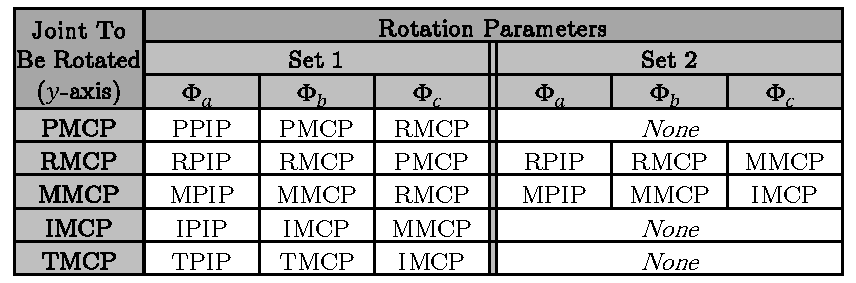
\includegraphics{figs/general/y_rots.pdf}
    \caption{Fully enumerated list of how each joint was rotated in the \underline{{\bfseries $\bm{y}$-axis}} for the inverse kinematics algorithm. See Equation \ref{eq:dotproduct} in Section \ref{sec:sd:d:ex}. Where a joint to be rotated has two sets of $\bm{\Phi}_a$, $\bm{\Phi}_b$, and $\bm{\Phi}_c$ vectors, the combination that produces the greatest magnitude of $\alpha$ in absolute terms with Equation \ref{eq:dotproduct} is chosen. See Figure \ref{fig:sd:hand} for details on the joint names.}
    \label{tb:yrots}
\end{table}

To calculate the $x$ rotations for each MANO joint, the corresponding MSRA joint, as well as the previous and next joint is used in the above formula. For example, to calculate the $x$ rotation for the PIP rotation of the ring finger, the RMCP, RPIP, and RDIP joints are inputted into Equation \ref{eq:dotproduct} letting $\bm{\Phi}_a=$RMCP, $\bm{\Phi}_b=$RPIP, and $\bm{\Phi}_c=$RDIP.

% \subsection{Hand shape}
% The shape of the hand can be changed by changing the Cartesian coordinates of each joint in the hand.

\begin{figure}
    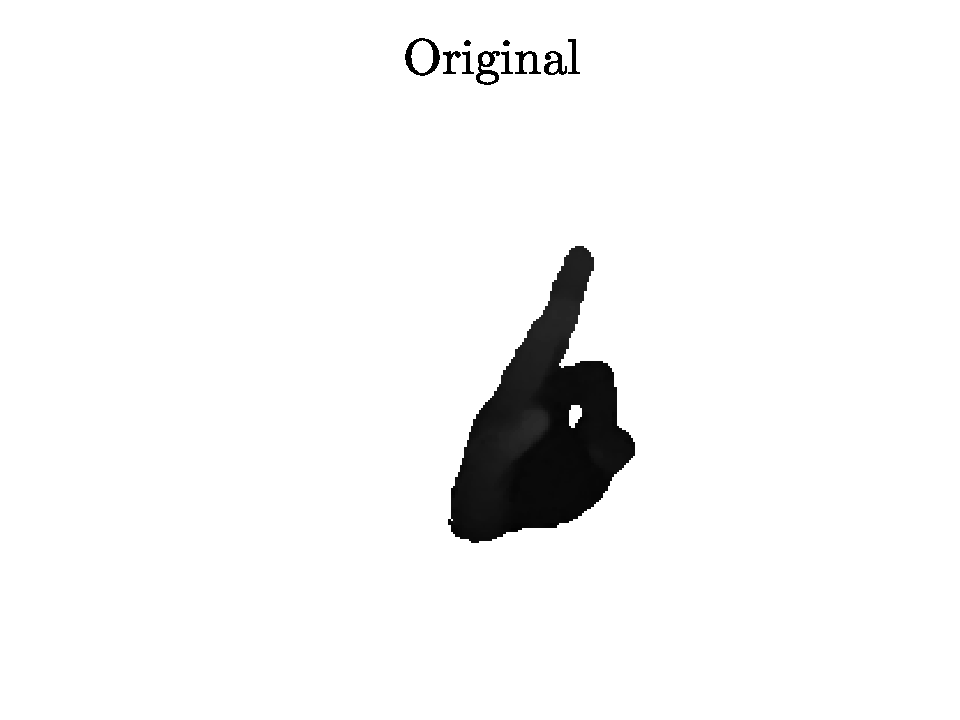
\includegraphics[width=0.48\linewidth]{figs/d_mano/original1.pdf}
    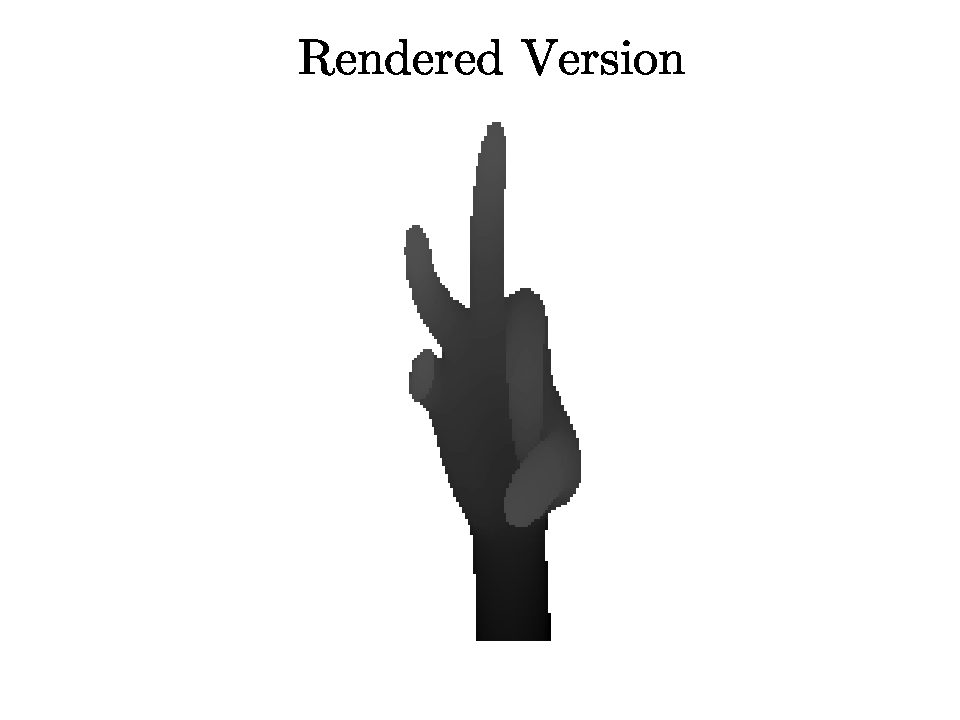
\includegraphics[width=0.48\linewidth]{figs/d_mano/rendered1.pdf}
    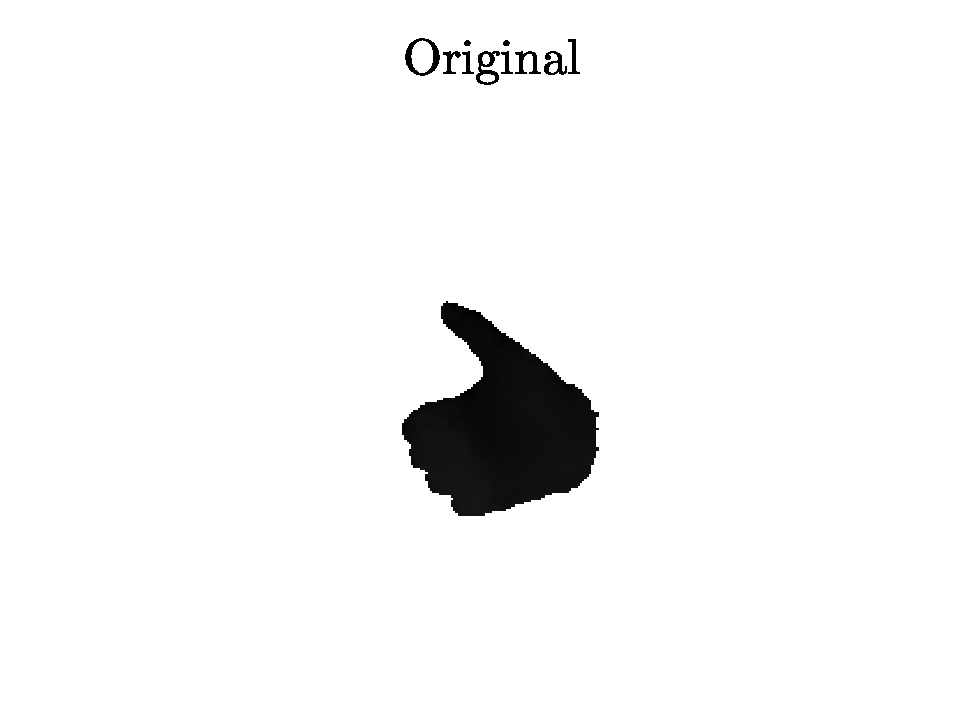
\includegraphics[width=0.48\linewidth]{figs/d_mano/original2.pdf}
    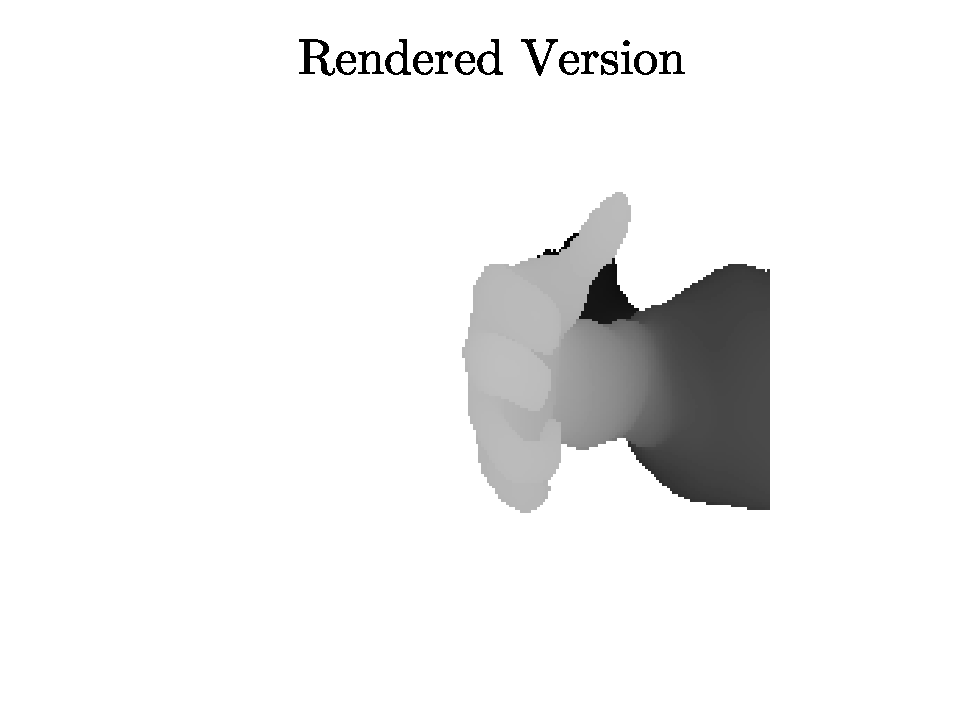
\includegraphics[width=0.48\linewidth]{figs/d_mano/rendered2.pdf}
    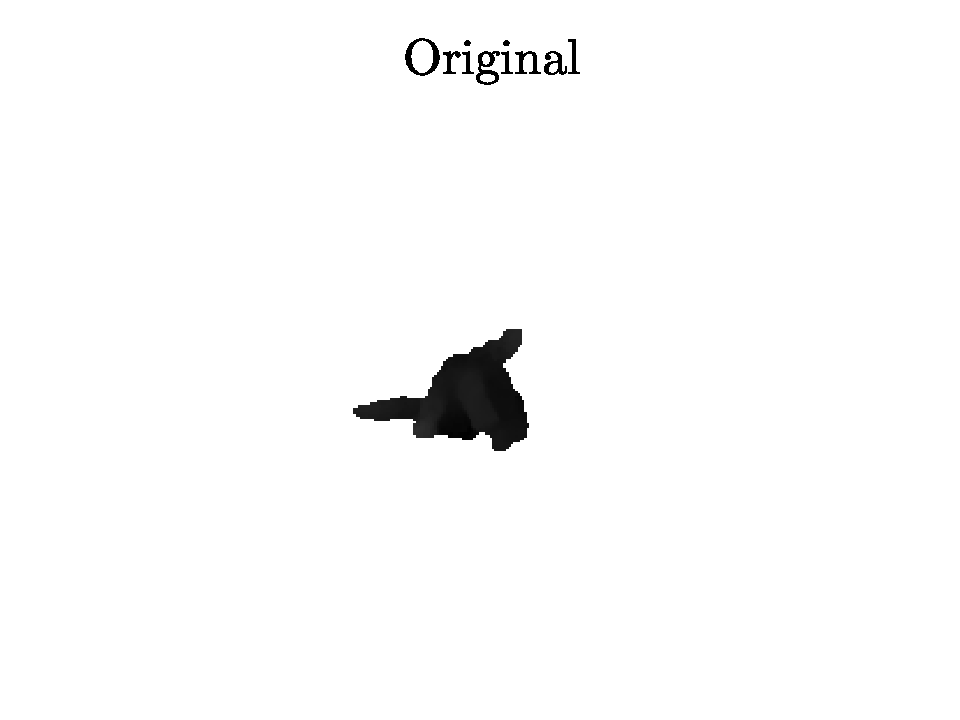
\includegraphics[width=0.48\linewidth]{figs/d_mano/original3.pdf}
    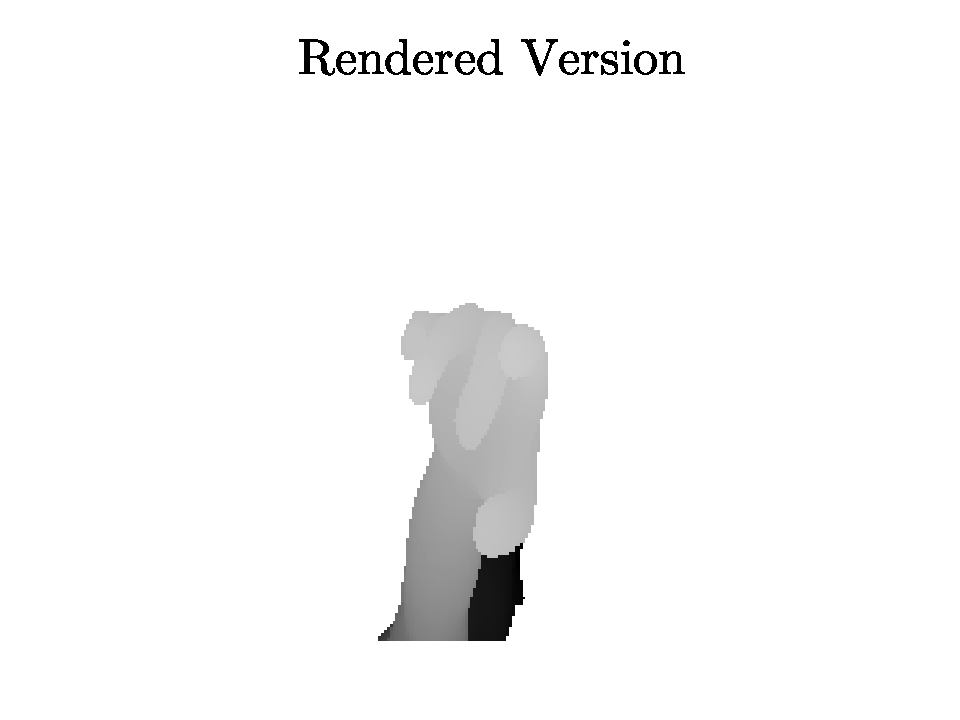
\includegraphics[width=0.48\linewidth]{figs/d_mano/rendered3.pdf}
    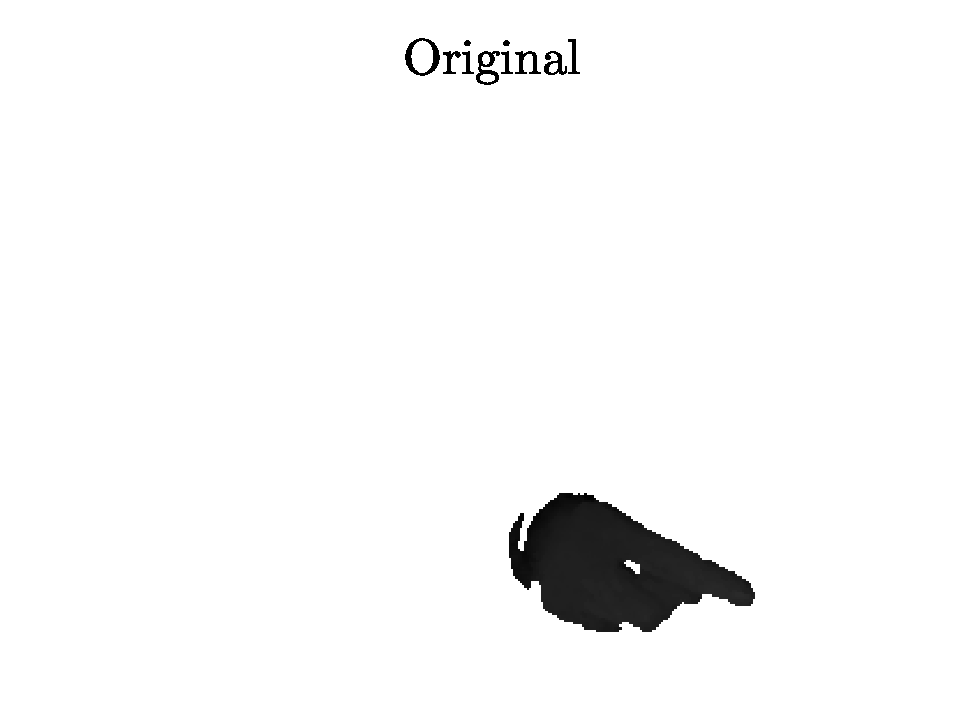
\includegraphics[width=0.48\linewidth]{figs/d_mano/original4.pdf}
    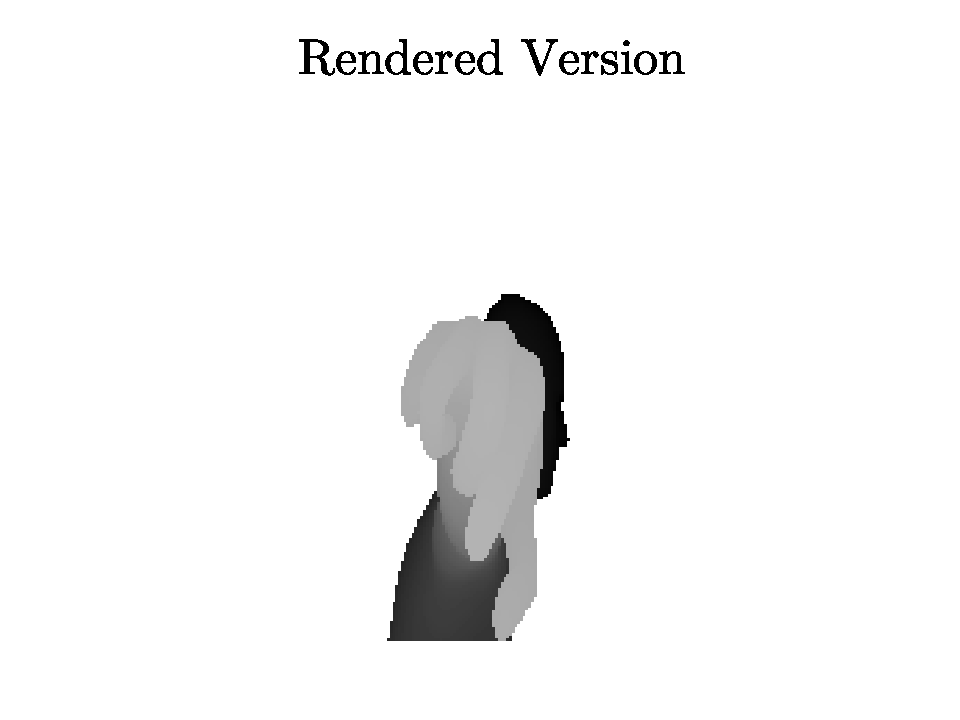
\includegraphics[width=0.48\linewidth]{figs/d_mano/rendered4.pdf}
    % 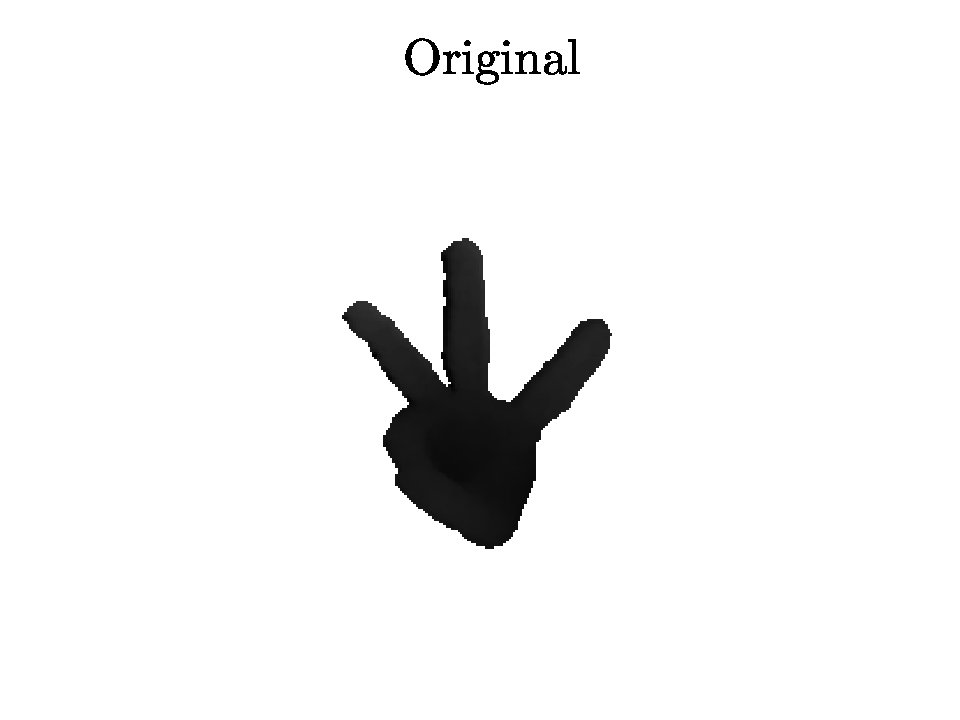
\includegraphics[width=220px]{figs/d_mano/original5.png}
    % 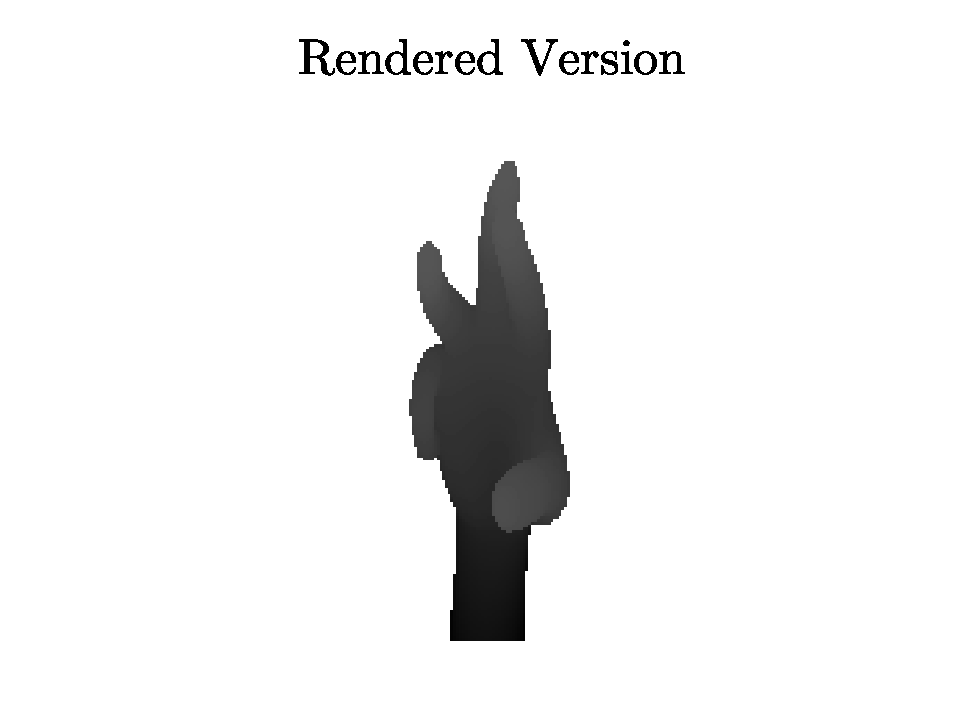
\includegraphics[width=220px]{figs/d_mano/rendered5.png}
\caption{Examples of images generated by trying to recreate the MSRA dataset. Note that the difference in colour is not significant and is dependent on the visualisation method only. The visible body is also segmented in training.}
\label{fig:sd:d}
\end{figure}

\subsubsection{Camera}
\label{sec:sd:d:cam}
The camera in Maya is the point in the scene where the renderer views from. It takes six parameters, three for Cartesian coordinates, and three for rotation: roll, pitch, and yaw ($\bm{R}_x$, $\bm{R}_y$, and $\bm{R}_z$). The camera for generating synthetic data is focused on the palm of the hand. The radius is set to a constant value, and the camera is always pointing towards a fixed point in the palm of the hand $P$, and it is moved by giving it the pitch, roll, and yaw parameters.

To achieve this, the camera is initially placed at point $[0, 0, r]$, where $r$ is the distance to the palm of the hand. Using the three rotation parameters, this point is rotated on the $x$, $y$, and $z$ axes by $\bm{R}_x$, $\bm{R}_y$, and $\bm{R}_z$ respectively. That rotated point is then translated to look at the hand by summing it by $P$, the resultant value is the new position in 3D space for the camera. The camera is then rotated by the same parameters $\bm{R}_x$, $\bm{R}_y$, and $\bm{R}_z$. This means that the camera will always be focused on the hand regardless of the input parameters $\bm{R}_x$, $\bm{R}_y$, and $\bm{R}_z$. The values of $\bm{R}_x$, $\bm{R}_y$, and $\bm{R}_z$ are obtained thus. The wrist and Index MCP coordinates are subtracted from each other to get a 3D vector describing the global rotation of the hand. The $x$, $y$, and $z$ rotations are then found using the right-angled triangle definition $\alpha=\arctan{\frac{a}{b}}$. The hyperparameters for this method were optimised by iterating over different values. This iterative method works by generating a small dataset (e.g. 1000 images), and testing the performance on the V2V-Posenet model that has been trained on the MSRA dataset.

This method does not robustly recreate the camera perspective found in the MSRA dataset, and unfortunately, the original MSRA dataset does not contain camera data.

\subsubsection{Normalising rendered image}
The process is the same as is described in Section \ref{sec:sd:nd:norm}.

\section{Transfer Learning}
% TODO: Correct MSRA count
\begin{figure}
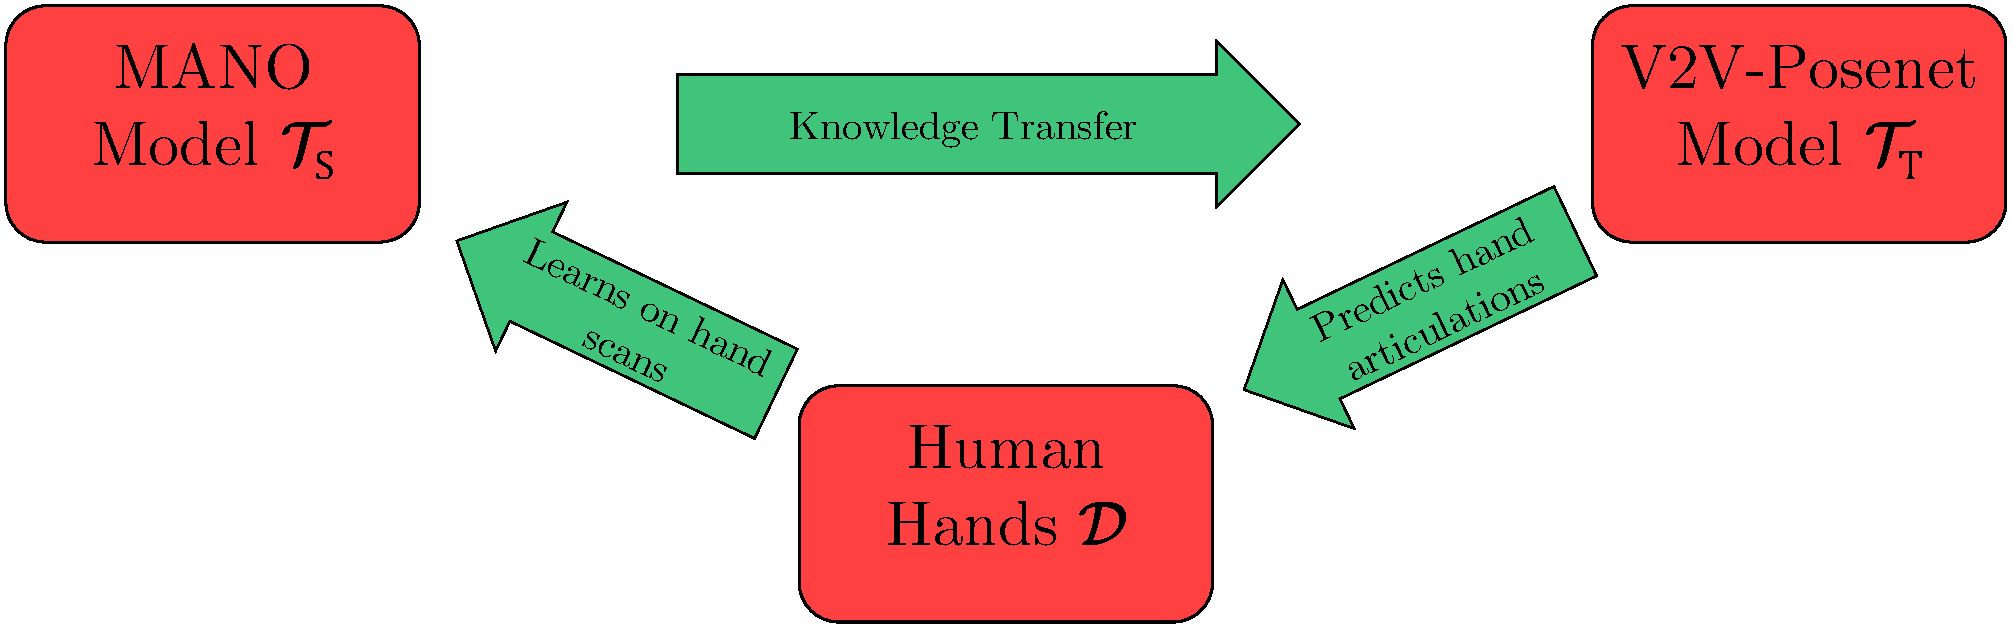
\includegraphics[width=\linewidth]{figs/general/knowledge_transfer.pdf}
\caption{High level overview of knowledge transfer in terms of training a hand tracking model using a synthetic hand generator. A task is denoted by $\mathcal{T}$, and a domain of data is denoted by $\mathcal{D}$.}
\label{fig:ktex}
\end{figure}
Formally, training a hand tracking system on synthetic data is a form of Transfer Learning, or knowledge transfer. Transfer learning is the idea of transferring the knowledge gained from training one model to another model \cite{pan2009survey}. The theory is that although the two tasks may be different, there may be some aspects of that knowledge that can be transferred, which reduces the need for new expensive labelled data. For example, if a CNN model has been trained to find if there are cars in an image, when training a CNN system to find if there are lorries in the image, there might be aspects of the knowledge in the car classification model that can be transferred to the lorry classification model. In practice, an example of how that can be achieved is by reusing the weights of some of the layers in the car CNN for the truck CNN and training only the end layers of that truck CNN. The key questions for Transfer Learning are: when should this approach be used, what knowledge should be transferred, and how should this be done in practice.

% Potentially bullshitting here
% The concept of what knowledge is is a notoriously vague topic, and this dissertation is not about Epistemology. However the topic is slightly easier to grasp when referring to data. Data and knowledge are different, and it is arguable that one of the main purposes of a computer is to gain knowledge from data. That is why certain computing tasks such as hand tracking are difficult. We as humans can observe an image of a hand and instantly know what the hand is doing, this knowledge is stored as data in the form of an image, but for a computer to extract this same knowledge is not so easy. The previous section has discussed many of the advances made in hand tracking, but they all using some form of CNN, and for the most part, we do not know how they work, because we don't know how the knowledge of a hand is encoded in the data of an image.

It is important to distinguish transfer learning from machine learning. In machine learning, a task is learned {\slshape from scratch} with training data. A successful machine learning task will train a model entirely on a dataset that is within the domain of the future examples that it is trying to predict. Using the example in Figure \ref{fig:mlex}, this model has learned to classify data into classes {\slshape red}, {\slshape green}, and {\slshape blue}. It learns these classifications given input data $x_1$ and $x_2$. Mathematically, this model can predict data from any domain, but it is only likely to be correct for data that it learned from. For example, the point marked with `?' lies in an ambiguous domain space, and we cannot be sure what class it belongs to. In contrast, in this dissertation the knowledge of the hand has already been learned in the MANO model, and the task is simply to transfer that knowledge to the V2V-Posenet model, the goal is to be able to train the V2V-Posenet model to learn from synthetic data without ever having to use real data.

\begin{figure}[H]
    \centering
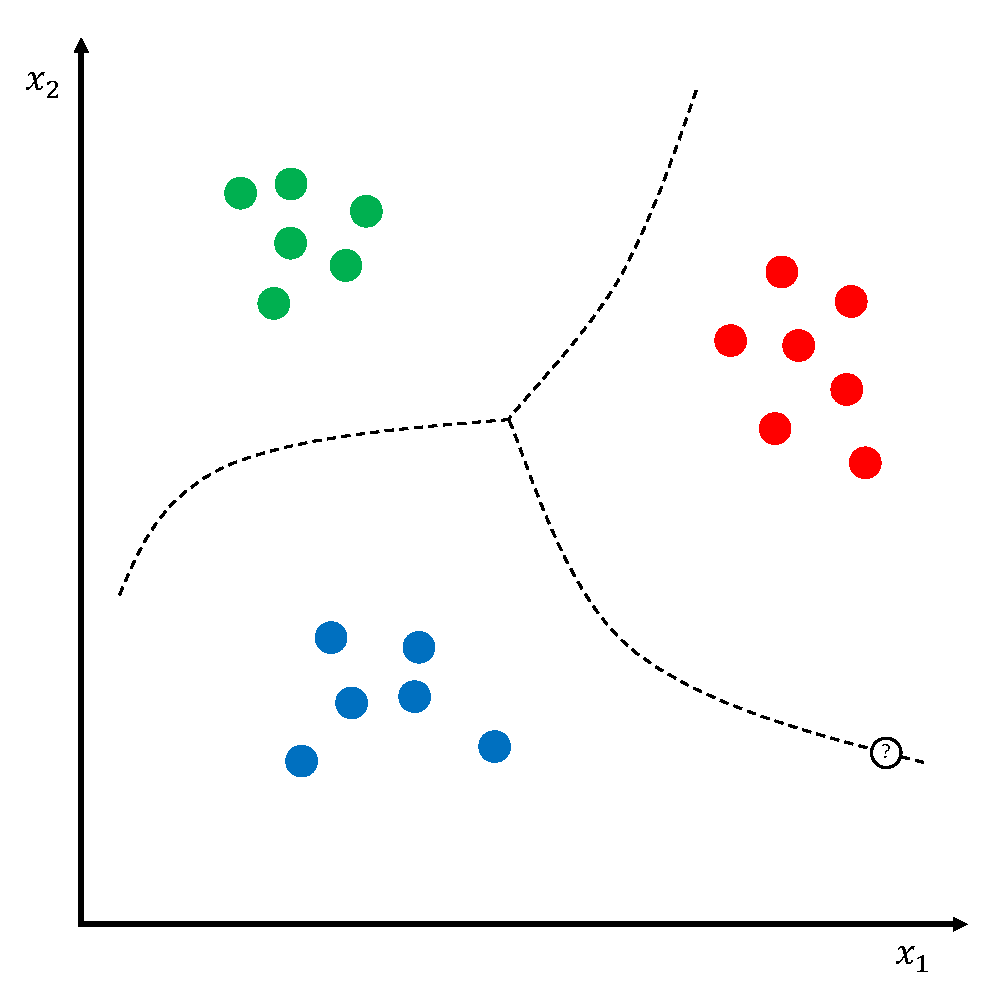
\includegraphics[width=210px]{figs/general/ml_example.pdf}
\caption{A toy example example of machine learning. This model learns to classify input data $\{x_1, x_2\}$ into three classes; red, green, and blue.}
\label{fig:mlex}
\end{figure}

The question of when transfer learning should be used can be answered by asking if {\slshape negative transfer} has occurred. {\slshape Negative transfer} is where the data from the source model leads to the reduced performance of the target model. In general, an example of when this can occur is when the two tasks are too dissimilar. In the context of hand tracking, it is important that the method used to achieve transfer learning is robust. In hand tracking, the occurance of {\slshape negative transfer} is determined by comparing how the model performs with real data versus synthetic data.

In terms of answering what to transfer, it is worth first reflecting on what the synthetic hand generation model is, and what the hand tracking model is. The synthetic hand generation model knows about the structure of the hand and how that is related to 3D space, and by giving it plausible articulations, that can be transferred to the hand tracking model.po Using the the terminology in \cite{pan2009survey}, the process of training a hand tracking system with synthetic data is an Inductive Transfer Learning task. In the context of this, the MANO model is the source task $\mathcal{T}_S$, and the target task $\mathcal{T}_T$ is the V2V-Posenet model. Both tasks have a common domain of human hands $\mathcal{D}$. A high level illustration of this concept is shown in Figure \ref{fig:ktex}.

%The source and target domains are both human hands, therefore they are the same, but the tasks are different. On a high level, the task of the MANO model is to generate a realistic synthetic representation of the human hand, the task of the V2V-Posenet model is to predict a set of keypoints from an inout mesh hand.

% MANO is learnt on a small amount of subjects and data, it uses the prior of the human, which is transferred to V2V.
\chapter{Experimental Setup}

This section discusses practical considerations related to the experiments undertaken in this dissertation. The important details of the hand tracking system used are discussed in Section \ref{sec:htm}. The details of the nature of the real dataset used in this dissertation are described in Section \ref{sec:es:msradset}. The performance metric of the hand tracking system used is defined in Section \ref{sec:pm}, this is particularly important as it is central to how the performance of a dataset is evaluated. Internal testing of the experimental setup is discussed in Section \ref{sec:sd:st}. Details of the experiments performed are discussed in Section \ref{es:exp}. Finally, miscellaneous matters are discussed in Section \ref{sec:sd:misc}.

\label{chap:es}
\section{Hand Tracking Model}
\label{sec:htm}
The V2V-Posenet model\cite{moon2018v2v} is used as the hand tracking system for training on, an overview of the network can be seen in Figure \ref{fig:v2vposenet}. It takes a depthmap $\bm{Z}$ as an input, and a 3D vector $\bm{v}$ denoting the centre of the hand in $\bm{Z}$ in 3D space. For this dissertation, where depthmap $\bm{Z}$ has an image resolution of $(a\times b)$, $\bm{v}_x = \frac{a}{2}$ and $\bm{v}_y=\frac{b}{2}$ and $\bm{v}_z = \bm{Z}_{\frac{a}{2},\frac{b}{2}}$. It outputs 3D predicted joints $\bm{\Phi}$ given a depthmap image $\bm{Z}$. Knowledge of the pipeline of this model is critical for generating the correct synthetic data. In the pipeline, the input depthmap is converted to a Point Cloud using $\bm{v}$ as a basis. In the context of this experiment, a Point Cloud is defined as an array of 3D vertices that describes the shape of an object in 3D space. Given that this is generated from a planar depth image, the Point Cloud does not define the entire surface of the hand. As such, self occlusions will also be visible in the Point Cloud. The algorithm for converting from a depthmap to a Point Cloud takes the indices of a pixel as an $x$, $y$ coordinate pair, and the value in that pixel as the $z$ coordinate. Points which are greater than a certain radius away from $\bm{v}$ are discarded, thus acting as a segmentation step between foreground and background. This Point Cloud is then turned into a voxel representation. Voxels are the 3D analogue to 2D pixels, and in the case of this setup, it is the 3D analogue to a 2D binary image. Formally, it is a 3D tensor, and can be seen as a verbose version of the Point Cloud.

An open source implementation of V2V-Posenet written in Python3 was used for this dissertation\footnote{\url{https://github.com/dragonbook/V2V-PoseNet-pytorch} (accessed 29th April 2020)}.

\section{MSRA Dataset}
\label{sec:es:msradset}
As previously mentioned, the MSRA dataset\cite{sun2015cascaded} is used as a baseline to compare the synthetic dataset. The MSRA dataset consists of depth images of nine subjects, and each subject performs seventeen gestures drawn from American Sign Language, to which there are approximately five-hundred frames each\footnote{\url{https://jimmysuen.github.io/txt/cvpr15\_MSRAHandGestureDB\_readme.txt} (accessed 29th April 2020)}. The dataset is split 90/10 for training and testing respectively. The implementation described in Section \ref{sec:htm} contains code for training on the MSRA dataset and it was not substantially modified.

\section{Performance Metrics}
\label{sec:pm}
\begin{figure}
    \centering
\includegraphics[width=0.8\linewidth]{figs/general/performance_metric.pdf}
\caption{A visualisation of the {\slshape Global Error} performance metric. The prediction and groundtruth are shown in blue and red respectively. The performance metric measures the average distance for each joint between the prediction and groundtruth, denoted for this example by the dotted black line. Each $\bm{\Phi}_{n}$ corresponds to a keypoint as in Figure \ref{fig:sd:hand}.}
\end{figure}
The performance metrics discussed in this section are the cornerstone from which synthetic data is compared with real data. As previously discussed, the goal of a hand tracking system is to extract information about a hand from an image of a hand, and one way of evaluating the hand tracking system's performance is by using the metrics described below. Therefore, the questions asked about synthetic hand data in this dissertation are answered using these metrics.

The primary performance metric used is mean per-joint error, as used in\cite{sun2015cascaded}. This performance metric shall be referred to as {\slshape Global Error}. Specifically, for {\slshape each joint}, the average euclidian distance (in millimeters) in 3D space is computed between the groundtruth keypoint $\bm{\mathrm{Y}}^{i}_{n,m}$ and predicted keypoint $\bm{\mathrm{Y}}^{o}_{n,m}$. An important implication of this is that the prediction could predict the correct articulation of the hand, but the per-joint error is still high because the global orientation or location of $\bm{\mathrm{Y}}^{i}_{n,m}$ is different to $\bm{\mathrm{Y}}^{o}_{n,m}$. The model must therefore aim to correctly predict orientation as well as articulation to perform well on this metric.

% \begin{equation}
%     d\Big(\bm{a}, \bm{b}\Big) = \sqrt{(\bm{a}_x-\bm{b}_x)^2+(\bm{a}_y-\bm{b}_y)^2+(\bm{a}_z-\bm{b}_z)^2}
% \end{equation}

There are $K$ images in the test dataset, and the hand tracking model predicts $N$ joints $\bm{\Phi}$ for each image $\bm{Z}$. $E^G$ is the average error for all joints, and $E^{G}_{n}$ denotes the average error for an individual joint $\bm{\Phi}_n$ (e.g. the per-joint error for the index MCP joint).
\begin{equation}
E^{G}_{n} = \frac{1}{K}\sum_{m=1}^{K} ||\bm{\mathrm{Y}}^{i}_{m,n} - \bm{\mathrm{Y}}^{o}_{m,n}||
\end{equation}
\begin{equation}
    E^{G} = \frac{1}{N}\sum_{k=1}^{N} E^{G}_{k}
\end{equation}

Through empirical observation, it was found that the V2V-Posenet model would often correctly predict the {\slshape articulation} and global {\slshape orientation} of the hand correctly, but not the global {\slshape position}. To account for situations where the model predicts the articulation and orientation correctly, but not the global position in 3D space, the following metric is also used. The above metric is modified by translating $\bm{\Phi}$ by the difference between the predicted and groundtruth values for the location of this wrist. This performance metric shall be referred to as {\slshape Local Error}. This means that the error for the wrist joint will be zero (thus this value is not reported in the local error metric). This second metric exists to provide more insight into performance. While the former metric is most important to optimise for a robust hand tracking system, this second metric can provide an intermediate goal to achieve in optimising the hand tracking model.

\begin{equation}
    E^{L}_{n} = \frac{1}{K}\sum_{m=1}^{K} ||\bm{\mathrm{Y}}^{i}_{m,n} + (\bm{\mathrm{Y}}^{o}_{m,n} + (\bm{\mathrm{Y}}^{i}_{m,0} - \bm{\mathrm{Y}}^{o}_{m,0}))||
\end{equation}
\begin{equation}
    E^{L} = \frac{1}{n}\sum_{k=1}^{N} E^{L}_{k}
\end{equation}

Typically, the scale that a hand lies within in local space is {\slshape approximately} $200mm$, that is the maximum span of an adult human hand. The precise value of this range is not important, but it does serve to illustrate how the above performance metrics are interpreted, particularly the second metric. For example, if the average per-joint error of one joint is $80mm$, that is far away, if it is $800mm$, then there is likely something very wrong with the system, and if it is $8mm$, that is perhaps a reasonable average error. There is no exact interpretation to this however, which is why a baseline exists to judge experimental results.

As discussed above, the MSRA dataset is used as the baseline for this experiment. The crux of this dissertation is to evaluate the merits of using synthetic data for training a hand tracking system. To answer this question, the V2V-Posenet model is trained and tested using the respective training sets of MSRA, which produces a particular error value. The answer is provided by comparing the performance of training the V2V-Posenet model with the MSRA dataset versus training it with the synthetic datasets.

% There are three datasets to consider, the existing MSRA dataset, as well as two datasets that I generate; non-deterministic and deterministic synthetic datasets generated using the MANO model. The two datasets that I generate are split into a training and test set in the same size and proportion to MSRA (67893 and 8498 respectively). For the baseline of this dissertation., the V2V-Posenet model is trained for five epochs with the MSRA training dataset, and validated on the equivalent test set. The error that this gives, based on the performance metric in Section \ref{sec:pm} is the baseline, and this forms the foundation from which the rest of the experiments are drawn. The goal of this dissertation is to asses.

\section{Software Testing}
\label{sec:sd:st}
Software testing is the primary method used for improving the synthetic data pipeline. Software testing for this dissertation and the evaluation of the merits of using synthetic data are two separate concerns. While the latter is evaluated using the performance metrics in Section \ref{sec:pm}, software testing refers to the performance of the internal components of the synthetic data generation system. The performance metric is directly reliant on the internal performance of this system, and the performance metric {\slshape might} suffer because of a bad design of the synthetic data pipeline, and not because my hypothesis about synthetic data is false. It is imperative that the synthetic data pipeline is optimal so that the performance metric in Section \ref{sec:pm} solely answers the hypothesis, and not a failing in my design of the pipeline. To address this concern, different tests were devised to evaluate the performance

In both the synthetic data generation pipelines, these are aspects that I believe are liable to failing.

\subsection{Data Visualisation}
\label{sec:es:st:dv}
\begin{figure}
\includegraphics[width=\linewidth]{figs/general/voxelisation.pdf}
\caption{A diagram of the preprocessing steps for the V2V-Posenet model, from input depthmap image $\bm{Z}$ and centre $\bm{v}$ to voxels, this voxelised representation is then passed into the 3D CNN. The two red boxes for {\slshape Point Cloud Visualisation} and {\slshape Voxel Visualisation} denote the two visualisation stages described in Section \ref{sec:es:st:dv}.}
\label{fig:prevoxels}
\end{figure}
Visualisation served as the backbone of software testing in this dissertation. Ideally, unit testing or some other sort of numerical test would be used, but given the complicated nature of the data being handled, I am not aware of any reliable unit testing regimen. The following parts describe the individual visualisation tests that were performed.

\subsubsection{Depthmap Visualisation}
This step visualises the conversion of the mesh outputted by MANO into the depthmap, as well as the normalisation of this image. This step was important for seeing whether the camera was behaving as expected, as well as visualising the domain of the foreground pixels and ensuring that there is a clear boundary between these foreground pixels and the background. Examples can be seen in Figure \ref{fig:sd:nd} and Figure \ref{fig:sd:d}.

\subsubsection{Pointcloud Visualisation}
The conversion of the depthmap to the pointcloud it one of the most important steps in the pipeline. An example of this can be seen in Figure \ref{fig:es:pc}. As previously described, the step of converting the depthmap to a Point Cloud uses a 3D centre point as a reference to the `centre' $\bm{v}$ of the hand, and all points further than a certain distance to this point are discarded. In Figure \ref{fig:es:pc}, this centre is denoted by the confluence of the three thin red lines. The threshold in which points beyond $\bm{v}$ are discarded is denoted by the green sphere. The purpose of this step is to ensure that most points lie within this green sphere. The definition of {\slshape most} is defined by my empirical observation of the MSRA dataset visualised at this step. It was found that {\slshape most}, but not all points describing the hand lie within this green sphere. The parameters that can be optimised in this step are the centre point of the image. This step was implemented with {\slshape Matplotlib}.

\begin{figure}
\includegraphics[width=0.5\linewidth]{figs/visualisation/pcloud0.pdf}
\includegraphics[width=0.5\linewidth]{figs/visualisation/pcloud1.pdf}
\includegraphics[width=0.5\linewidth]{figs/visualisation/pcloud2.pdf}
\includegraphics[width=0.5\linewidth]{figs/visualisation/vox0.pdf}
\includegraphics[width=0.5\linewidth]{figs/visualisation/vox1.pdf}
\includegraphics[width=0.5\linewidth]{figs/visualisation/vox2.pdf}
\caption{Examples the visualisation tools for the pointcloud (top row and middle left) and voxelisation (bottom row and middle right). For the pointcloud, all blue points that fall within the green sphere are voxelised, note as well that the background pixel points are not shown.}
\label{fig:es:pc}
\end{figure}

\subsubsection{Voxel Visualisation}
Converting from pointcloud to voxels is the last step in the pipeline before the data is passed to the V2V-Posenet model. This step is largely robust for a given pointcloud representation since it is part of the implementation of the V2V-Posenet model that is used for this dissertation. It does however serve to confirm that the pointcloud visualisation step itself works. This step also was implemented with {\slshape Matplotlib}. Examples are also in Figure \ref{fig:es:pc}.

% \begin{figure}
% \includegraphics[width=140px]{figs/visualisation/vox0.png}
% \includegraphics[width=140px]{figs/visualisation/vox1.png}
% \includegraphics[width=140px]{figs/visualisation/vox2.png}
% \caption{Examples the visualisation tool for voxels from different perspectives, this uses the same input image used in Figure \ref{fig:es:pc}.}
% \label{fig:es:vox}
% \end{figure}

% To evaluate this, a simple metric of time is used. The overall time, as well as time per image is recorded. This became particularly important for rotations, I had previously used a liib


\section{Experiments}
\label{es:exp}
This section details the experiments undertaken in this dissertation. All experiments involved training the V2V-Posenet model for 5 epochs with a batch size of 12. Every dataset consists of 67893 training images, and 8498 test images.

\subsection{Baseline}
\label{es:ex:base}
The baseline of this dissertation is training the V2V-Posenet model with the real MSRA training dataset, it is then validated with the MSRA test dataset. It is also validated with the test datasets for the Random MANO and IK MANO datasets too.

\subsection{Analysis Of Synthetic Data}
The Random MANO and IK MANO datasets are investigated separately. Both respective training datasets are used to train the V2V-Posenet model under two scenarios; random initialisation of the V2V-Posenet weights, and one where the weights obtained from training the V2V-Posenet model on the MSRA training dataset are used as a base. In total, this gives four models obtained from training with synthetic data. Each of these four models are tested with the respective test synthetic dataset, and the MSRA test dataset, which gives eight testing scenarios. There are two error metrics described in Section \ref{sec:pm}, so this gives sixteen sets of results.

% As mentioned previously, the first experiment for this dissertation is training the V2V-Posenet model with the MSRA dataset to give a baseline. For both synthetic datasets, the V2V-Posenet model is then trained under two starting points, one where the weights of the V2V-Posenet model weights are initialised at random as is how the model is trained originally with the MSRA dataset, and one where the weights from the MSRA-trained baseline are used. In these four scenarios, the model is trained for five epochs as is the case for the baseline. For each training scenario, two testing scenarios are used. One where the test synthetic dataset is used against the performance metric, and one where the MSRA test dataset is used. In all, 16 sets of values are produced, which are summarised in Section \ref{chap:res}.

% \section{Maya}
% As previously mentioned, Maya \footnote{\url{https://autodesk.com/maya} (accessed 29th April 2020)} is the programme that was used to generate the synthetic dataset deterministically. In order for the problem to scale well, the process was entirely automated to the extent using the built-in Python implementation, which notably in the 2020 version uses version {\slshape 2.7.11}, which led to certain practical challenges using up-to-date libraries. As well as this, the generation of synthetic data had the ability to benefit from parallel execution, specifically when the render for a particular image was complete by Arnold, some further processing was required which could be done in parallel.

% \subsection{Execution Model}
% A producer-consumer execution model was used to achieve this, were the main programme, Maya Python spawns a child process using the \verb|subprocess.Popen| function call in the standard library. Very specifically, the \verb|subprocess.Popen| call is a wrapper for the {\slshape Fork-exec} technique. The {\slshape Fork-exec} technique is where a process creates a copy of itself using the \verb|fork()| call (available on all POSIX operating systems) which makes a clone of the parent process, so the child process has the replica, but seperate address space, and the same set of instructions, the two programmes can distinguish each other by the fact that \verb|fork()| returns the child's processor ID in the parent process, and zero in the child process. This is followed by the \verb|exec()| in the child process, which replaces the programme's machine instructions and address space with the new programme's, while keeping the same processor ID, and the parent continues with its own execution \footnote{\url{https://github.com/python/cpython/blob/master/Modules/_posixsubprocess.c} (accessed 29th April 2020)}.

% The child process runs a modern version of Python to perform the post-processing of each depth image. The parent and child processes communicate using a pipeline. Every time a new image is rendered in Maya, it saves the file to disk, when this occurs, the name, path, and grountruth of that image are passed to the child process in the pipeline, and the child performs the processing based on this information. In the execution pattern of the child, it waits for this information to be given to it. In order to strive towards deterministic execution, a \verb|SIGALARM| is set to check a boolean that says whether the programme should stop when waiting for input, and if it receives nothing in the next three seconds, and that boolean is set to true, the child process stops. In the parent process, a wrapper class for calling the child process is implemented, and when that wrapper class is garbage-collected, it send a \verb|SIGTERM| signal to the child, in the child, this sets the boolean to true, and if it is in the middle of processing an image, it will complete that first, and it will continue to process whatever is still in the pipeline before stopping.

\section{Miscellaneous}
\label{sec:sd:misc}
\subsection{Execution Model}
\subsubsection{}{Random MANO Dataset}
The MANO parameters $\bm{\beta}$ and $\bm{\theta}$ are determined at random for generating the Random MANO dataset. To make the generation of the data is made consistent over different runs, the random number generator is seeded with a constant value. When training, the images are generated at runtime before the model is trained and are stored in a temporary directory using the {\slshape tempfile} library\footnote{\url{https://docs.python.org/3.7/library/tempfile.html} (accessed 29th April 2020)} in Python. To give a fair comparison with the MSRA dataset, the same size for the training and test sets are used at 67893 and 8498 respectively. A different seed for the random number generator is used for training and testing. 

\subsubsection{IK MANO Dataset}
As previously mentioned, recreating the real dataset is achieved in Maya\footnote{\url{https://autodesk.com/maya} (accessed 29th April 2020)}, a 3D computer graphics programme. The actual renderer used is Arnold\footnote{\url{https://www.arnoldrenderer.com} (accessed 29th April 2020)}. This was running on a different computer to the one used to run the V2V-Posenet model, and it lacked a GPU which meant that it was not feasible to generate the dataset in real time with training the model (it takes 12 hours and 53 minutes to generate the training and test dataset, or 607 milliseconds per image). Given the size of the dataset, the process was scripted. Maya comes with a Python environment for writing scripts which has API calls for scripting tasks within Maya. An important implication of using Maya Python is that it uses Python 2.7.11, which was released in December 2015 and lacks the support of many modern libraries. As well as this, it does not come with {\slshape PIP}, a common package manager in Python, which made it more challenging to use certain third party libraries. As a way around this problem, as well as to make the execution of the programme more efficient, two processes were used in the synthetic data generation process; Maya Python, as well as another process running Python 3. This was achieved using the {\slshape subprocess} library in Python\footnote{\url{https://docs.python.org/release/2.7.11/library/subprocess.html} (accessed 29th April 2020)}.

The calculation of the camera position, hand articulation, as well as the rendering happend within the Maya Python process. The Python 3 process did extra processing on the image (using the Python {\slshape subprocess} library), this consisted of normalising the rendered images, then compressing them to save disk space (using the numpy.savez\footnote{\url{https://numpy.org/devdocs/reference/generated/numpy.savez.html} (accessed 29th April 2020)} method). The execution of these processes worked in a producer-consumer model. The child process runs a modern version of Python to perform the post-processing of each depth image. The parent and child processes communicate using a Unix-style pipeline. Every time a new image is rendered in Maya, it saves the file to disk, when this occurs, the name, path, and grountruth of that image are passed to the child process in the pipeline, and the child performs the processing based on this information. In the execution pattern of the child, it waits for this information to be given to it. In order to strive towards deterministic execution, a \verb|SIGALARM| is set to check a boolean that says whether the programme should stop when waiting for input, and if it receives nothing in the next three seconds, and that boolean is set to true, the child process stops. In the parent process, a wrapper class for calling the child process is implemented, and when that wrapper class is garbage-collected, it send a \verb|SIGTERM| signal to the child, in the child, this sets the boolean to true, and if it is in the middle of processing an image, it will complete that first, and it will continue to process whatever is still in the pipeline before stopping.

\subsection{Execution Speed}
Execution speed refers to how quickly the synthetic data pipeline can execute, from generating, processing, training, and testing on the synthetic data. While this is not necessarily needed in terms of ensuring that the synthetic data pipeline is optimal towards improving the performance metric, it is important towards improving the speed of the pipeline itself, since it means that less time can wasted between per development cycle. Since the software for this dissertation was written in Python, this primarily focussed on the optimal use of libraries within Python. Python is an Interpreted language, and is not compiled to machine code before execution so code written in it executes slowly in comparison to software that is compiled (such as C, C++ and Fortran). Some libraries in Python are written in compiled languages however. This means therefore that Python code should aim to offset as many instructions within the code to libraries that are written in compiled languages as possible.

\subsection{Computers}
Two computers were used in the experiments. The rational behind this is that one computer had a GPU which is needed for modern CNN training tasks, but it was not portable and lacked a GUI, a laptop was also used. The first computer, which was used for data visualisation and generating the MSRA-based synthetic dataset with Maya ran using a 2.6 GHz 6-core Intel i7 8850H, with 16GB of 2400MHz DDR4 RAM running macOS 10.15.3. The second computer used for the rest of the tasks in this dissertation used a 3.6 GHz 6-core AMD Ryzen 5 3600 with 32GB of 2400MHz DDR4 RAM and an Nvidia RTX 2060S with 8GB of GDDR6 RAM, running Ubuntu Server 18.04 LTS.

Since two computers were used for this dissertation, a practical concern during this project was how to communicate between the two computers. {\slshape Secure shell} (SSH) proved to be the most useful tool to achieve this. The internet connection for the server does not allow for port forwarding, which means that it cannot be an SSH server that is accessible from the internet. To solve this problem, a VPN server was deployed on Amazon Web Services (AWS). The AWS-based VPN server had a permanent connection to this computer, so when an SSH connection was made to the server from my laptop, it connected via this VPN server. Given the nature of this project, large quantities of data transfer were required, and AWS charges for this beyond a threshold, so the server did not connect to the internet via the VPN save for SSH communication. For the data visualisation tasks described in Section \ref{sec:es:st:dv}, the programme in the server interacts at different stages of the V2V-Posenet pipeline to extract information, and writes this data as a Python script, which can be copy and pasted onto my laptop. Given the small file size, this proved to be computationally feasible. 
\chapter{Results}
\label{chap:res}
\definecolor{dd_green}{HTML}{00ff00}
\definecolor{dd_red}{HTML}{ff0000}
\definecolor{dd_yellowgreen}{HTML}{88ff00}
\definecolor{dd_yellow}{HTML}{ffff00}
\definecolor{dd_yelloworange}{HTML}{ff8800}
Section \ref{ap:sum} provides a summary of the baseline and results using the {\slshape Global Error} $E^G$ and {\slshape Local Error} $E^L$ metrics. Sections thereafter provide the full baseline and results using the per-joint {\slshape Global Error} $E^G_n$ and {\slshape Local Error} $E^L_n$ metrics. See Section \ref{sec:pm} for details on the performance metrics. The real dataset is the {\slshape MSRA} dataset, and the synthetic datasets are the {\slshape Random MANO} dataset and {\slshape IK MANO} dataset, see Section \ref{sec:sdgm} for details. See Figure \ref{fig:sd:hand} for details on the joint names.

% Good results (around 10 mm) are highlighted in {\bfseries\colorbox{dd_green}{green}}, and bad results (around 100 mm) are highlighted in {\bfseries\colorbox{dd_red}{red}}, results in between (around 50 mm) are defined by appropriate shades of {\bfseries\colorbox{dd_yellow}{yellow}} and {\bfseries\colorbox{dd_yelloworange}{orange}}.

Results are colour-coded, with good results (around 10mm) highlighted in {\bfseries\colorbox{dd_green}{green}}, progressively worse results are highlighted in shades of {\bfseries\colorbox{dd_yellow}{yellow}} and {\bfseries\colorbox{dd_yelloworange}{orange}}, with the worst results highlighted in {\bfseries\colorbox{dd_red}{red}} (> 90mm).
\FloatBarrier\section{Summary}
\label{ap:sum}

\begin{table}[!ht]
    \centering
    \includegraphics[width=0.7\linewidth]{figs/general/baseline.pdf}
    \caption{The experimental baseline, showing the results when the model is first trained on the MSRA training dataset, then tested on the test MSRA dataset and test synthetic datasets.}
    \end{table}

\begin{table}[!ht]
        \centering
        \includegraphics[width=\linewidth]{figs/general/results.pdf}
        \caption{Summary of results over all experiments undertaken. Each experiment reports the average error over all joints for the two metrics described in Section \ref{sec:pm}. See Section \ref{es:exp} for details on the experiments performed.}
    \end{table}


% \FloatBarrier\section{Full Results}
\label{ap:fullres}
\setlength{\tabcolsep}{0.05cm}
\FloatBarrier\section{Baseline Tests}
% All results are in millimeters.
\label{sec:ap:base}
\begin{table}[!ht]
    \begin{tabular}{|c|c|c|c|c|c|c|c|c|c|c|}
    \hline
    \cellcolor[HTML]{40ff00}{\bfseries Wrist} & \cellcolor[HTML]{00ff00}{\bfseries IMCP} & \cellcolor[HTML]{40ff00}{\bfseries IPIP} & \cellcolor[HTML]{40ff00}{\bfseries IDIP} & \cellcolor[HTML]{40ff00}{\bfseries ITIP} & \cellcolor[HTML]{00ff00}{\bfseries MMCP} & \cellcolor[HTML]{00ff00}{\bfseries MPIP} & \cellcolor[HTML]{00ff00}{\bfseries MDIP}  \\
    \cellcolor[HTML]{40ff00}$\,\,\,$10.20 mm & \cellcolor[HTML]{00ff00}$\,\,\,\,\,\,$8.82 mm & \cellcolor[HTML]{40ff00}$\,\,\,$10.10 mm & \cellcolor[HTML]{40ff00}$\,\,\,$10.88 mm & \cellcolor[HTML]{40ff00}$\,\,\,$13.40 mm & \cellcolor[HTML]{00ff00}$\,\,\,\,\,\,$7.33 mm & \cellcolor[HTML]{00ff00}$\,\,\,\,\,\,$8.23 mm & \cellcolor[HTML]{00ff00}$\,\,\,\,\,\,$9.87 mm\\
    \hline
    \cellcolor[HTML]{40ff00}{\bfseries MTIP} & \cellcolor[HTML]{00ff00}{\bfseries RMCP} & \cellcolor[HTML]{00ff00}{\bfseries RPIP} & \cellcolor[HTML]{00ff00}{\bfseries RDIP} & \cellcolor[HTML]{40ff00}{\bfseries RTIP} & \cellcolor[HTML]{00ff00}{\bfseries PMCP} & \cellcolor[HTML]{00ff00}{\bfseries PPIP} & \cellcolor[HTML]{00ff00}{\bfseries PDIP}  \\
    \cellcolor[HTML]{40ff00}$\,\,\,$13.05 mm & \cellcolor[HTML]{00ff00}$\,\,\,\,\,\,$7.56 mm & \cellcolor[HTML]{00ff00}$\,\,\,\,\,\,$7.88 mm & \cellcolor[HTML]{00ff00}$\,\,\,\,\,\,$9.54 mm & \cellcolor[HTML]{40ff00}$\,\,\,$12.68 mm & \cellcolor[HTML]{00ff00}$\,\,\,\,\,\,$9.13 mm & \cellcolor[HTML]{00ff00}$\,\,\,\,\,\,$8.57 mm & \cellcolor[HTML]{00ff00}$\,\,\,\,\,\,$9.27 mm\\
    \hline
    \cellcolor[HTML]{40ff00}{\bfseries PTIP} & \cellcolor[HTML]{00ff00}{\bfseries TMCP} & \cellcolor[HTML]{40ff00}{\bfseries TPIP} & \cellcolor[HTML]{40ff00}{\bfseries PDIP} & \cellcolor[HTML]{40ff00}{\bfseries TTIP} & \cellcolor[HTML]{40ff00}{\bfseries Average}  \\
    \cellcolor[HTML]{40ff00}$\,\,\,$12.04 mm & \cellcolor[HTML]{00ff00}$\,\,\,\,\,\,$9.74 mm & \cellcolor[HTML]{40ff00}$\,\,\,$11.02 mm & \cellcolor[HTML]{40ff00}$\,\,\,$12.00 mm & \cellcolor[HTML]{40ff00}$\,\,\,$15.55 mm & \cellcolor[HTML]{40ff00}$\,\,\,$10.33 mm \\
    \cline{1-6}
    \end{tabular}
    \caption{Global error when model trained with the MSRA dataset initialised with random weights and tested on the MSRA test dataset.}
    \label{tb:baseline_msra:g}
    \end{table}
    \begin{table}[!ht]
    \begin{tabular}{|c|c|c|c|c|c|c|c|c|c|c|}
    \hline
    {\bfseries Wrist} & \cellcolor[HTML]{40ff00}{\bfseries IMCP} & \cellcolor[HTML]{40ff00}{\bfseries IPIP} & \cellcolor[HTML]{40ff00}{\bfseries IDIP} & \cellcolor[HTML]{40ff00}{\bfseries ITIP} & \cellcolor[HTML]{40ff00}{\bfseries MMCP} & \cellcolor[HTML]{40ff00}{\bfseries MPIP} & \cellcolor[HTML]{40ff00}{\bfseries MDIP}  \\
    N/A mm & \cellcolor[HTML]{40ff00}$\,\,\,$10.82 mm & \cellcolor[HTML]{40ff00}$\,\,\,$13.18 mm & \cellcolor[HTML]{40ff00}$\,\,\,$14.75 mm & \cellcolor[HTML]{40ff00}$\,\,\,$17.31 mm & \cellcolor[HTML]{40ff00}$\,\,\,$10.76 mm & \cellcolor[HTML]{40ff00}$\,\,\,$13.45 mm & \cellcolor[HTML]{40ff00}$\,\,\,$15.20 mm\\
    \hline
    \cellcolor[HTML]{40ff00}{\bfseries MTIP} & \cellcolor[HTML]{40ff00}{\bfseries RMCP} & \cellcolor[HTML]{40ff00}{\bfseries RPIP} & \cellcolor[HTML]{40ff00}{\bfseries RDIP} & \cellcolor[HTML]{40ff00}{\bfseries RTIP} & \cellcolor[HTML]{40ff00}{\bfseries PMCP} & \cellcolor[HTML]{40ff00}{\bfseries PPIP} & \cellcolor[HTML]{40ff00}{\bfseries PDIP}  \\
    \cellcolor[HTML]{40ff00}$\,\,\,$17.71 mm & \cellcolor[HTML]{40ff00}$\,\,\,$11.59 mm & \cellcolor[HTML]{40ff00}$\,\,\,$13.63 mm & \cellcolor[HTML]{40ff00}$\,\,\,$15.21 mm & \cellcolor[HTML]{40ff00}$\,\,\,$17.47 mm & \cellcolor[HTML]{40ff00}$\,\,\,$13.20 mm & \cellcolor[HTML]{40ff00}$\,\,\,$13.57 mm & \cellcolor[HTML]{40ff00}$\,\,\,$14.14 mm\\
    \hline
    \cellcolor[HTML]{40ff00}{\bfseries PTIP} & \cellcolor[HTML]{00ff00}{\bfseries TMCP} & \cellcolor[HTML]{40ff00}{\bfseries TPIP} & \cellcolor[HTML]{40ff00}{\bfseries PDIP} & \cellcolor[HTML]{40ff00}{\bfseries TTIP} & \cellcolor[HTML]{40ff00}{\bfseries Average}  \\
    \cellcolor[HTML]{40ff00}$\,\,\,$16.62 mm & \cellcolor[HTML]{00ff00}$\,\,\,\,\,\,$8.72 mm & \cellcolor[HTML]{40ff00}$\,\,\,$12.60 mm & \cellcolor[HTML]{40ff00}$\,\,\,$15.07 mm & \cellcolor[HTML]{40ff00}$\,\,\,$18.86 mm & \cellcolor[HTML]{40ff00}$\,\,\,$14.19 mm \\
    \cline{1-6}
    \end{tabular}
    \caption{Local error when model trained with the MSRA dataset initialised with random weights and tested on the MSRA test dataset.}
    \label{tb:baseline_msra:l}
    \end{table}
\begin{table}[!ht]
    \begin{tabular}{|c|c|c|c|c|c|c|c|c|c|c|}
    \hline
    \cellcolor[HTML]{ff0000}{\bfseries Wrist} & \cellcolor[HTML]{ff0000}{\bfseries IMCP} & \cellcolor[HTML]{ff2500}{\bfseries IPIP} & \cellcolor[HTML]{ff2500}{\bfseries IDIP} & \cellcolor[HTML]{ff2500}{\bfseries ITIP} & \cellcolor[HTML]{ff2500}{\bfseries MMCP} & \cellcolor[HTML]{ff7500}{\bfseries MPIP} & \cellcolor[HTML]{ff7500}{\bfseries MDIP}  \\
    \cellcolor[HTML]{ff0000}123.25 mm & \cellcolor[HTML]{ff0000}105.61 mm & \cellcolor[HTML]{ff2500}$\,\,\,$84.00 mm & \cellcolor[HTML]{ff2500}$\,\,\,$86.13 mm & \cellcolor[HTML]{ff2500}$\,\,\,$84.01 mm & \cellcolor[HTML]{ff2500}$\,\,\,$82.64 mm & \cellcolor[HTML]{ff7500}$\,\,\,$79.98 mm & \cellcolor[HTML]{ff7500}$\,\,\,$70.77 mm\\
    \hline
    \cellcolor[HTML]{ff7500}{\bfseries MTIP} & \cellcolor[HTML]{ff7500}{\bfseries RMCP} & \cellcolor[HTML]{ff7500}{\bfseries RPIP} & \cellcolor[HTML]{ff2500}{\bfseries RDIP} & \cellcolor[HTML]{ff7500}{\bfseries RTIP} & \cellcolor[HTML]{ff2500}{\bfseries PMCP} & \cellcolor[HTML]{ff7500}{\bfseries PPIP} & \cellcolor[HTML]{ff2500}{\bfseries PDIP}  \\
    \cellcolor[HTML]{ff7500}$\,\,\,$72.60 mm & \cellcolor[HTML]{ff7500}$\,\,\,$77.96 mm & \cellcolor[HTML]{ff7500}$\,\,\,$72.01 mm & \cellcolor[HTML]{ff2500}$\,\,\,$81.24 mm & \cellcolor[HTML]{ff7500}$\,\,\,$72.84 mm & \cellcolor[HTML]{ff2500}$\,\,\,$84.75 mm & \cellcolor[HTML]{ff7500}$\,\,\,$79.84 mm & \cellcolor[HTML]{ff2500}$\,\,\,$86.36 mm\\
    \hline
    \cellcolor[HTML]{ff2500}{\bfseries PTIP} & \cellcolor[HTML]{ff0000}{\bfseries TMCP} & \cellcolor[HTML]{ff0000}{\bfseries TPIP} & \cellcolor[HTML]{ff0000}{\bfseries PDIP} & \cellcolor[HTML]{ff0000}{\bfseries TTIP} & \cellcolor[HTML]{ff0000}{\bfseries Average}  \\
    \cellcolor[HTML]{ff2500}$\,\,\,$85.79 mm & \cellcolor[HTML]{ff0000}138.94 mm & \cellcolor[HTML]{ff0000}118.87 mm & \cellcolor[HTML]{ff0000}102.89 mm & \cellcolor[HTML]{ff0000}119.04 mm & \cellcolor[HTML]{ff0000}$\,\,\,$90.93 mm \\
    \cline{1-6}
    \end{tabular}
    \caption{Global error when model trained with the MSRA dataset initialised with random weights and tested on the Random MANO dataset.}
    \label{tb:baseline_mano:g}
    \end{table}
    \begin{table}[!ht]
    \begin{tabular}{|c|c|c|c|c|c|c|c|c|c|c|}
    \hline
    {\bfseries Wrist} & \cellcolor[HTML]{ff0000}{\bfseries IMCP} & \cellcolor[HTML]{ff0000}{\bfseries IPIP} & \cellcolor[HTML]{ff0000}{\bfseries IDIP} & \cellcolor[HTML]{ff0000}{\bfseries ITIP} & \cellcolor[HTML]{ff0000}{\bfseries MMCP} & \cellcolor[HTML]{ff0000}{\bfseries MPIP} & \cellcolor[HTML]{ff0000}{\bfseries MDIP}  \\
    N/A mm & \cellcolor[HTML]{ff0000}121.88 mm & \cellcolor[HTML]{ff0000}117.93 mm & \cellcolor[HTML]{ff0000}127.07 mm & \cellcolor[HTML]{ff0000}130.78 mm & \cellcolor[HTML]{ff0000}115.38 mm & \cellcolor[HTML]{ff0000}113.78 mm & \cellcolor[HTML]{ff0000}109.93 mm\\
    \hline
    \cellcolor[HTML]{ff0000}{\bfseries MTIP} & \cellcolor[HTML]{ff0000}{\bfseries RMCP} & \cellcolor[HTML]{ff0000}{\bfseries RPIP} & \cellcolor[HTML]{ff0000}{\bfseries RDIP} & \cellcolor[HTML]{ff0000}{\bfseries RTIP} & \cellcolor[HTML]{ff0000}{\bfseries PMCP} & \cellcolor[HTML]{ff0000}{\bfseries PPIP} & \cellcolor[HTML]{ff0000}{\bfseries PDIP}  \\
    \cellcolor[HTML]{ff0000}121.37 mm & \cellcolor[HTML]{ff0000}107.26 mm & \cellcolor[HTML]{ff0000}105.41 mm & \cellcolor[HTML]{ff0000}115.54 mm & \cellcolor[HTML]{ff0000}114.41 mm & \cellcolor[HTML]{ff0000}114.18 mm & \cellcolor[HTML]{ff0000}124.42 mm & \cellcolor[HTML]{ff0000}108.09 mm\\
    \hline
    \cellcolor[HTML]{ff0000}{\bfseries PTIP} & \cellcolor[HTML]{ff0000}{\bfseries TMCP} & \cellcolor[HTML]{ff0000}{\bfseries TPIP} & \cellcolor[HTML]{ff0000}{\bfseries PDIP} & \cellcolor[HTML]{ff0000}{\bfseries TTIP} & \cellcolor[HTML]{ff0000}{\bfseries Average}  \\
    \cellcolor[HTML]{ff0000}112.18 mm & \cellcolor[HTML]{ff0000}136.50 mm & \cellcolor[HTML]{ff0000}128.28 mm & \cellcolor[HTML]{ff0000}136.64 mm & \cellcolor[HTML]{ff0000}116.67 mm & \cellcolor[HTML]{ff0000}118.89 mm \\
    \cline{1-6}
    \end{tabular}
    \caption{Local error when model trained with the MSRA dataset initialised with random weights and tested on the Random MANO test dataset.}
    \label{tb:baseline_mano:l}
    \end{table}
\begin{table}[!ht]
    \begin{tabular}{|c|c|c|c|c|c|c|c|c|c|c|}
    \hline
    \cellcolor[HTML]{ff7500}{\bfseries Wrist} & \cellcolor[HTML]{ff7500}{\bfseries IMCP} & \cellcolor[HTML]{ff2500}{\bfseries IPIP} & \cellcolor[HTML]{ff0000}{\bfseries IDIP} & \cellcolor[HTML]{ff0000}{\bfseries ITIP} & \cellcolor[HTML]{ff7500}{\bfseries MMCP} & \cellcolor[HTML]{ff2500}{\bfseries MPIP} & \cellcolor[HTML]{ff0000}{\bfseries MDIP}  \\
    \cellcolor[HTML]{ff7500}$\,\,\,$73.79 mm & \cellcolor[HTML]{ff7500}$\,\,\,$75.54 mm & \cellcolor[HTML]{ff2500}$\,\,\,$86.05 mm & \cellcolor[HTML]{ff0000}$\,\,\,$96.61 mm & \cellcolor[HTML]{ff0000}108.52 mm & \cellcolor[HTML]{ff7500}$\,\,\,$73.57 mm & \cellcolor[HTML]{ff2500}$\,\,\,$89.94 mm & \cellcolor[HTML]{ff0000}100.02 mm\\
    \hline
    \cellcolor[HTML]{ff0000}{\bfseries MTIP} & \cellcolor[HTML]{ff7500}{\bfseries RMCP} & \cellcolor[HTML]{ff2500}{\bfseries RPIP} & \cellcolor[HTML]{ff0000}{\bfseries RDIP} & \cellcolor[HTML]{ff0000}{\bfseries RTIP} & \cellcolor[HTML]{ff7500}{\bfseries PMCP} & \cellcolor[HTML]{ff2500}{\bfseries PPIP} & \cellcolor[HTML]{ff0000}{\bfseries PDIP}  \\
    \cellcolor[HTML]{ff0000}112.83 mm & \cellcolor[HTML]{ff7500}$\,\,\,$75.50 mm & \cellcolor[HTML]{ff2500}$\,\,\,$87.29 mm & \cellcolor[HTML]{ff0000}$\,\,\,$92.89 mm & \cellcolor[HTML]{ff0000}$\,\,\,$98.37 mm & \cellcolor[HTML]{ff7500}$\,\,\,$78.78 mm & \cellcolor[HTML]{ff2500}$\,\,\,$86.27 mm & \cellcolor[HTML]{ff0000}$\,\,\,$92.02 mm\\
    \hline
    \cellcolor[HTML]{ff0000}{\bfseries PTIP} & \cellcolor[HTML]{ff7500}{\bfseries TMCP} & \cellcolor[HTML]{ff7500}{\bfseries TPIP} & \cellcolor[HTML]{ff2500}{\bfseries PDIP} & \cellcolor[HTML]{ff0000}{\bfseries TTIP} & \cellcolor[HTML]{ff2500}{\bfseries Average}  \\
    \cellcolor[HTML]{ff0000}$\,\,\,$98.80 mm & \cellcolor[HTML]{ff7500}$\,\,\,$70.36 mm & \cellcolor[HTML]{ff7500}$\,\,\,$77.56 mm & \cellcolor[HTML]{ff2500}$\,\,\,$85.33 mm & \cellcolor[HTML]{ff0000}$\,\,\,$99.91 mm & \cellcolor[HTML]{ff2500}$\,\,\,$88.57 mm \\
    \cline{1-6}
    \end{tabular}
    \caption{Global error when model trained with the MSRA dataset initialised with random weights and tested on the IK MANO test dataset.}
    \label{tb:baseline_maya:g}
    \end{table}
    \begin{table}[!ht]
    \begin{tabular}{|c|c|c|c|c|c|c|c|c|c|c|}
    \hline
    {\bfseries Wrist} & \cellcolor[HTML]{ff8000}{\bfseries IMCP} & \cellcolor[HTML]{ff2500}{\bfseries IPIP} & \cellcolor[HTML]{ff0000}{\bfseries IDIP} & \cellcolor[HTML]{ff0000}{\bfseries ITIP} & \cellcolor[HTML]{ff8000}{\bfseries MMCP} & \cellcolor[HTML]{ff0000}{\bfseries MPIP} & \cellcolor[HTML]{ff0000}{\bfseries MDIP}  \\
    N/A mm & \cellcolor[HTML]{ff8000}$\,\,\,$67.93 mm & \cellcolor[HTML]{ff2500}$\,\,\,$84.63 mm & \cellcolor[HTML]{ff0000}$\,\,\,$96.64 mm & \cellcolor[HTML]{ff0000}108.02 mm & \cellcolor[HTML]{ff8000}$\,\,\,$69.45 mm & \cellcolor[HTML]{ff0000}$\,\,\,$93.01 mm & \cellcolor[HTML]{ff0000}103.37 mm\\
    \hline
    \cellcolor[HTML]{ff0000}{\bfseries MTIP} & \cellcolor[HTML]{ff7500}{\bfseries RMCP} & \cellcolor[HTML]{ff0000}{\bfseries RPIP} & \cellcolor[HTML]{ff0000}{\bfseries RDIP} & \cellcolor[HTML]{ff0000}{\bfseries RTIP} & \cellcolor[HTML]{ff7500}{\bfseries PMCP} & \cellcolor[HTML]{ff2500}{\bfseries PPIP} & \cellcolor[HTML]{ff0000}{\bfseries PDIP}  \\
    \cellcolor[HTML]{ff0000}115.10 mm & \cellcolor[HTML]{ff7500}$\,\,\,$71.51 mm & \cellcolor[HTML]{ff0000}$\,\,\,$90.29 mm & \cellcolor[HTML]{ff0000}$\,\,\,$96.56 mm & \cellcolor[HTML]{ff0000}100.27 mm & \cellcolor[HTML]{ff7500}$\,\,\,$75.71 mm & \cellcolor[HTML]{ff2500}$\,\,\,$88.43 mm & \cellcolor[HTML]{ff0000}$\,\,\,$94.82 mm\\
    \hline
    \cellcolor[HTML]{ff0000}{\bfseries PTIP} & \cellcolor[HTML]{ffff00}{\bfseries TMCP} & \cellcolor[HTML]{ff8000}{\bfseries TPIP} & \cellcolor[HTML]{ff7500}{\bfseries PDIP} & \cellcolor[HTML]{ff0000}{\bfseries TTIP} & \cellcolor[HTML]{ff2500}{\bfseries Average}  \\
    \cellcolor[HTML]{ff0000}101.63 mm & \cellcolor[HTML]{ffff00}$\,\,\,$42.45 mm & \cellcolor[HTML]{ff8000}$\,\,\,$64.63 mm & \cellcolor[HTML]{ff7500}$\,\,\,$77.68 mm & \cellcolor[HTML]{ff0000}$\,\,\,$93.73 mm & \cellcolor[HTML]{ff2500}$\,\,\,$86.79 mm \\
    \cline{1-6}
    \end{tabular}
    \caption{Local error when model trained with the MSRA dataset initialised with random weights and tested on the IK MANO test dataset.}
    \label{tb:baseline_maya:l}
    \end{table}

\FloatBarrier\section{Training With The Random MANO Synthetic Dataset}
% All results are in millimeters.
\label{sec:ap:mano}
\begin{table}[!ht]
    \begin{tabular}{|c|c|c|c|c|c|c|c|c|c|c|}
    \hline
    \cellcolor[HTML]{00ff00}{\bfseries Wrist} & \cellcolor[HTML]{00ff00}{\bfseries IMCP} & \cellcolor[HTML]{00ff00}{\bfseries IPIP} & \cellcolor[HTML]{00ff00}{\bfseries IDIP} & \cellcolor[HTML]{40ff00}{\bfseries ITIP} & \cellcolor[HTML]{00ff00}{\bfseries MMCP} & \cellcolor[HTML]{00ff00}{\bfseries MPIP} & \cellcolor[HTML]{00ff00}{\bfseries MDIP}  \\
    \cellcolor[HTML]{00ff00}$\,\,\,\,\,\,$8.39 mm & \cellcolor[HTML]{00ff00}$\,\,\,\,\,\,$8.30 mm & \cellcolor[HTML]{00ff00}$\,\,\,\,\,\,$8.68 mm & \cellcolor[HTML]{00ff00}$\,\,\,\,\,\,$9.48 mm & \cellcolor[HTML]{40ff00}$\,\,\,$11.10 mm & \cellcolor[HTML]{00ff00}$\,\,\,\,\,\,$7.70 mm & \cellcolor[HTML]{00ff00}$\,\,\,\,\,\,$7.90 mm & \cellcolor[HTML]{00ff00}$\,\,\,\,\,\,$8.35 mm\\
    \hline
    \cellcolor[HTML]{00ff00}{\bfseries MTIP} & \cellcolor[HTML]{00ff00}{\bfseries RMCP} & \cellcolor[HTML]{00ff00}{\bfseries RPIP} & \cellcolor[HTML]{00ff00}{\bfseries RDIP} & \cellcolor[HTML]{40ff00}{\bfseries RTIP} & \cellcolor[HTML]{00ff00}{\bfseries PMCP} & \cellcolor[HTML]{00ff00}{\bfseries PPIP} & \cellcolor[HTML]{00ff00}{\bfseries PDIP}  \\
    \cellcolor[HTML]{00ff00}$\,\,\,\,\,\,$9.97 mm & \cellcolor[HTML]{00ff00}$\,\,\,\,\,\,$7.28 mm & \cellcolor[HTML]{00ff00}$\,\,\,\,\,\,$7.54 mm & \cellcolor[HTML]{00ff00}$\,\,\,\,\,\,$8.29 mm & \cellcolor[HTML]{40ff00}$\,\,\,$10.46 mm & \cellcolor[HTML]{00ff00}$\,\,\,\,\,\,$7.25 mm & \cellcolor[HTML]{00ff00}$\,\,\,\,\,\,$7.73 mm & \cellcolor[HTML]{00ff00}$\,\,\,\,\,\,$8.75 mm\\
    \hline
    \cellcolor[HTML]{40ff00}{\bfseries PTIP} & \cellcolor[HTML]{00ff00}{\bfseries TMCP} & \cellcolor[HTML]{00ff00}{\bfseries TPIP} & \cellcolor[HTML]{00ff00}{\bfseries PDIP} & \cellcolor[HTML]{40ff00}{\bfseries TTIP} & \cellcolor[HTML]{00ff00}{\bfseries Average}  \\
    \cellcolor[HTML]{40ff00}$\,\,\,$10.97 mm & \cellcolor[HTML]{00ff00}$\,\,\,\,\,\,$8.29 mm & \cellcolor[HTML]{00ff00}$\,\,\,\,\,\,$8.65 mm & \cellcolor[HTML]{00ff00}$\,\,\,\,\,\,$9.68 mm & \cellcolor[HTML]{40ff00}$\,\,\,$12.12 mm & \cellcolor[HTML]{00ff00}$\,\,\,\,\,\,$8.90 mm \\
    \cline{1-6}
    \end{tabular}
    \caption{Global error when model trained with Random MANO dataset initialised with random weights and tested on Random MANO test dataset.}
    \label{tb:orog}
    \end{table}
    \begin{table}[!ht]
    \begin{tabular}{|c|c|c|c|c|c|c|c|c|c|c|}
    \hline
    {\bfseries Wrist} & \cellcolor[HTML]{00ff00}{\bfseries IMCP} & \cellcolor[HTML]{00ff00}{\bfseries IPIP} & \cellcolor[HTML]{00ff00}{\bfseries IDIP} & \cellcolor[HTML]{00ff00}{\bfseries ITIP} & \cellcolor[HTML]{00ff00}{\bfseries MMCP} & \cellcolor[HTML]{00ff00}{\bfseries MPIP} & \cellcolor[HTML]{00ff00}{\bfseries MDIP}  \\
    N/A mm & \cellcolor[HTML]{00ff00}$\,\,\,\,\,\,$5.08 mm & \cellcolor[HTML]{00ff00}$\,\,\,\,\,\,$6.13 mm & \cellcolor[HTML]{00ff00}$\,\,\,\,\,\,$7.41 mm & \cellcolor[HTML]{00ff00}$\,\,\,\,\,\,$9.74 mm & \cellcolor[HTML]{00ff00}$\,\,\,\,\,\,$4.84 mm & \cellcolor[HTML]{00ff00}$\,\,\,\,\,\,$5.89 mm & \cellcolor[HTML]{00ff00}$\,\,\,\,\,\,$6.93 mm\\
    \hline
    \cellcolor[HTML]{00ff00}{\bfseries MTIP} & \cellcolor[HTML]{00ff00}{\bfseries RMCP} & \cellcolor[HTML]{00ff00}{\bfseries RPIP} & \cellcolor[HTML]{00ff00}{\bfseries RDIP} & \cellcolor[HTML]{00ff00}{\bfseries RTIP} & \cellcolor[HTML]{00ff00}{\bfseries PMCP} & \cellcolor[HTML]{00ff00}{\bfseries PPIP} & \cellcolor[HTML]{00ff00}{\bfseries PDIP}  \\
    \cellcolor[HTML]{00ff00}$\,\,\,\,\,\,$9.16 mm & \cellcolor[HTML]{00ff00}$\,\,\,\,\,\,$4.68 mm & \cellcolor[HTML]{00ff00}$\,\,\,\,\,\,$5.69 mm & \cellcolor[HTML]{00ff00}$\,\,\,\,\,\,$7.09 mm & \cellcolor[HTML]{00ff00}$\,\,\,\,\,\,$9.87 mm & \cellcolor[HTML]{00ff00}$\,\,\,\,\,\,$4.89 mm & \cellcolor[HTML]{00ff00}$\,\,\,\,\,\,$6.03 mm & \cellcolor[HTML]{00ff00}$\,\,\,\,\,\,$7.56 mm\\
    \hline
    \cellcolor[HTML]{40ff00}{\bfseries PTIP} & \cellcolor[HTML]{00ff00}{\bfseries TMCP} & \cellcolor[HTML]{00ff00}{\bfseries TPIP} & \cellcolor[HTML]{00ff00}{\bfseries PDIP} & \cellcolor[HTML]{40ff00}{\bfseries TTIP} & \cellcolor[HTML]{00ff00}{\bfseries Average}  \\
    \cellcolor[HTML]{40ff00}$\,\,\,$10.23 mm & \cellcolor[HTML]{00ff00}$\,\,\,\,\,\,$3.95 mm & \cellcolor[HTML]{00ff00}$\,\,\,\,\,\,$5.08 mm & \cellcolor[HTML]{00ff00}$\,\,\,\,\,\,$6.89 mm & \cellcolor[HTML]{40ff00}$\,\,\,$10.37 mm & \cellcolor[HTML]{00ff00}$\,\,\,\,\,\,$6.88 mm \\
    \cline{1-6}
    \end{tabular}
    \caption{Local error when model trained with Random MANO dataset initialised with random weights and tested on Random MANO test dataset.}
    \label{tb:orol}
    \end{table}
\begin{table}[!ht]
    \begin{tabular}{|c|c|c|c|c|c|c|c|c|c|c|}
    \hline
    \cellcolor[HTML]{ff7500}{\bfseries Wrist} & \cellcolor[HTML]{ff0000}{\bfseries IMCP} & \cellcolor[HTML]{ff0000}{\bfseries IPIP} & \cellcolor[HTML]{ff0000}{\bfseries IDIP} & \cellcolor[HTML]{ff0000}{\bfseries ITIP} & \cellcolor[HTML]{ff0000}{\bfseries MMCP} & \cellcolor[HTML]{ff0000}{\bfseries MPIP} & \cellcolor[HTML]{ff0000}{\bfseries MDIP}  \\
    \cellcolor[HTML]{ff7500}$\,\,\,$75.91 mm & \cellcolor[HTML]{ff0000}$\,\,\,$99.64 mm & \cellcolor[HTML]{ff0000}108.10 mm & \cellcolor[HTML]{ff0000}106.09 mm & \cellcolor[HTML]{ff0000}108.97 mm & \cellcolor[HTML]{ff0000}109.41 mm & \cellcolor[HTML]{ff0000}104.96 mm & \cellcolor[HTML]{ff0000}105.99 mm\\
    \hline
    \cellcolor[HTML]{ff0000}{\bfseries MTIP} & \cellcolor[HTML]{ff0000}{\bfseries RMCP} & \cellcolor[HTML]{ff0000}{\bfseries RPIP} & \cellcolor[HTML]{ff0000}{\bfseries RDIP} & \cellcolor[HTML]{ff0000}{\bfseries RTIP} & \cellcolor[HTML]{ff0000}{\bfseries PMCP} & \cellcolor[HTML]{ff0000}{\bfseries PPIP} & \cellcolor[HTML]{ff0000}{\bfseries PDIP}  \\
    \cellcolor[HTML]{ff0000}110.81 mm & \cellcolor[HTML]{ff0000}110.22 mm & \cellcolor[HTML]{ff0000}106.17 mm & \cellcolor[HTML]{ff0000}107.01 mm & \cellcolor[HTML]{ff0000}107.00 mm & \cellcolor[HTML]{ff0000}103.82 mm & \cellcolor[HTML]{ff0000}111.16 mm & \cellcolor[HTML]{ff0000}112.72 mm\\
    \hline
    \cellcolor[HTML]{ff0000}{\bfseries PTIP} & \cellcolor[HTML]{ff2500}{\bfseries TMCP} & \cellcolor[HTML]{ff0000}{\bfseries TPIP} & \cellcolor[HTML]{ff0000}{\bfseries PDIP} & \cellcolor[HTML]{ff0000}{\bfseries TTIP} & \cellcolor[HTML]{ff0000}{\bfseries Average}  \\
    \cellcolor[HTML]{ff0000}111.82 mm & \cellcolor[HTML]{ff2500}$\,\,\,$85.61 mm & \cellcolor[HTML]{ff0000}101.98 mm & \cellcolor[HTML]{ff0000}112.97 mm & \cellcolor[HTML]{ff0000}113.48 mm & \cellcolor[HTML]{ff0000}105.42 mm \\
    \cline{1-6}
    \end{tabular}
    \caption{Global error when model trained with Random MANO dataset initialised with random weights and tested on MSRA test dataset.}
    \label{tb:orag}
    \end{table}
    \begin{table}[!ht]
    \begin{tabular}{|c|c|c|c|c|c|c|c|c|c|c|}
    \hline
    {\bfseries Wrist} & \cellcolor[HTML]{ff0000}{\bfseries IMCP} & \cellcolor[HTML]{ff0000}{\bfseries IPIP} & \cellcolor[HTML]{ff0000}{\bfseries IDIP} & \cellcolor[HTML]{ff0000}{\bfseries ITIP} & \cellcolor[HTML]{ff0000}{\bfseries MMCP} & \cellcolor[HTML]{ff0000}{\bfseries MPIP} & \cellcolor[HTML]{ff0000}{\bfseries MDIP}  \\
    N/A mm & \cellcolor[HTML]{ff0000}109.93 mm & \cellcolor[HTML]{ff0000}121.02 mm & \cellcolor[HTML]{ff0000}120.88 mm & \cellcolor[HTML]{ff0000}126.14 mm & \cellcolor[HTML]{ff0000}121.30 mm & \cellcolor[HTML]{ff0000}126.35 mm & \cellcolor[HTML]{ff0000}126.83 mm\\
    \hline
    \cellcolor[HTML]{ff0000}{\bfseries MTIP} & \cellcolor[HTML]{ff0000}{\bfseries RMCP} & \cellcolor[HTML]{ff0000}{\bfseries RPIP} & \cellcolor[HTML]{ff0000}{\bfseries RDIP} & \cellcolor[HTML]{ff0000}{\bfseries RTIP} & \cellcolor[HTML]{ff0000}{\bfseries PMCP} & \cellcolor[HTML]{ff0000}{\bfseries PPIP} & \cellcolor[HTML]{ff0000}{\bfseries PDIP}  \\
    \cellcolor[HTML]{ff0000}130.08 mm & \cellcolor[HTML]{ff0000}123.69 mm & \cellcolor[HTML]{ff0000}128.24 mm & \cellcolor[HTML]{ff0000}127.39 mm & \cellcolor[HTML]{ff0000}125.41 mm & \cellcolor[HTML]{ff0000}117.20 mm & \cellcolor[HTML]{ff0000}130.32 mm & \cellcolor[HTML]{ff0000}133.18 mm\\
    \hline
    \cellcolor[HTML]{ff0000}{\bfseries PTIP} & \cellcolor[HTML]{ff8000}{\bfseries TMCP} & \cellcolor[HTML]{ff0000}{\bfseries TPIP} & \cellcolor[HTML]{ff0000}{\bfseries PDIP} & \cellcolor[HTML]{ff0000}{\bfseries TTIP} & \cellcolor[HTML]{ff0000}{\bfseries Average}  \\
    \cellcolor[HTML]{ff0000}133.56 mm & \cellcolor[HTML]{ff8000}$\,\,\,$68.03 mm & \cellcolor[HTML]{ff0000}$\,\,\,$99.87 mm & \cellcolor[HTML]{ff0000}114.25 mm & \cellcolor[HTML]{ff0000}118.20 mm & \cellcolor[HTML]{ff0000}120.09 mm \\
    \cline{1-6}
    \end{tabular}
    \caption{Local error when model trained with Random MANO dataset initialised with random weights and tested on MSRA test dataset.}
    \label{tb:oral}
    \end{table}
\begin{table}[!ht]
    \begin{tabular}{|c|c|c|c|c|c|c|c|c|c|c|}
    \hline
    \cellcolor[HTML]{00ff00}{\bfseries Wrist} & \cellcolor[HTML]{00ff00}{\bfseries IMCP} & \cellcolor[HTML]{00ff00}{\bfseries IPIP} & \cellcolor[HTML]{00ff00}{\bfseries IDIP} & \cellcolor[HTML]{40ff00}{\bfseries ITIP} & \cellcolor[HTML]{00ff00}{\bfseries MMCP} & \cellcolor[HTML]{00ff00}{\bfseries MPIP} & \cellcolor[HTML]{00ff00}{\bfseries MDIP}  \\
    \cellcolor[HTML]{00ff00}$\,\,\,\,\,\,$7.77 mm & \cellcolor[HTML]{00ff00}$\,\,\,\,\,\,$7.45 mm & \cellcolor[HTML]{00ff00}$\,\,\,\,\,\,$7.79 mm & \cellcolor[HTML]{00ff00}$\,\,\,\,\,\,$8.70 mm & \cellcolor[HTML]{40ff00}$\,\,\,$10.49 mm & \cellcolor[HTML]{00ff00}$\,\,\,\,\,\,$6.88 mm & \cellcolor[HTML]{00ff00}$\,\,\,\,\,\,$7.23 mm & \cellcolor[HTML]{00ff00}$\,\,\,\,\,\,$7.94 mm\\
    \hline
    \cellcolor[HTML]{00ff00}{\bfseries MTIP} & \cellcolor[HTML]{00ff00}{\bfseries RMCP} & \cellcolor[HTML]{00ff00}{\bfseries RPIP} & \cellcolor[HTML]{00ff00}{\bfseries RDIP} & \cellcolor[HTML]{00ff00}{\bfseries RTIP} & \cellcolor[HTML]{00ff00}{\bfseries PMCP} & \cellcolor[HTML]{00ff00}{\bfseries PPIP} & \cellcolor[HTML]{00ff00}{\bfseries PDIP}  \\
    \cellcolor[HTML]{00ff00}$\,\,\,\,\,\,$9.75 mm & \cellcolor[HTML]{00ff00}$\,\,\,\,\,\,$6.66 mm & \cellcolor[HTML]{00ff00}$\,\,\,\,\,\,$6.82 mm & \cellcolor[HTML]{00ff00}$\,\,\,\,\,\,$7.76 mm & \cellcolor[HTML]{00ff00}$\,\,\,\,\,\,$9.87 mm & \cellcolor[HTML]{00ff00}$\,\,\,\,\,\,$6.61 mm & \cellcolor[HTML]{00ff00}$\,\,\,\,\,\,$7.05 mm & \cellcolor[HTML]{00ff00}$\,\,\,\,\,\,$8.12 mm\\
    \hline
    \cellcolor[HTML]{40ff00}{\bfseries PTIP} & \cellcolor[HTML]{00ff00}{\bfseries TMCP} & \cellcolor[HTML]{00ff00}{\bfseries TPIP} & \cellcolor[HTML]{00ff00}{\bfseries PDIP} & \cellcolor[HTML]{40ff00}{\bfseries TTIP} & \cellcolor[HTML]{00ff00}{\bfseries Average}  \\
    \cellcolor[HTML]{40ff00}$\,\,\,$10.19 mm & \cellcolor[HTML]{00ff00}$\,\,\,\,\,\,$7.79 mm & \cellcolor[HTML]{00ff00}$\,\,\,\,\,\,$7.96 mm & \cellcolor[HTML]{00ff00}$\,\,\,\,\,\,$9.12 mm & \cellcolor[HTML]{40ff00}$\,\,\,$11.29 mm & \cellcolor[HTML]{00ff00}$\,\,\,\,\,\,$8.25 mm \\
    \cline{1-6}
    \end{tabular}
    \caption{Local error when model trained with Random MANO dataset initialised with MSRA weights and tested on Random MANO test dataset.}
    \label{tb:omog}
    \end{table}
    \begin{table}[!ht]
    \begin{tabular}{|c|c|c|c|c|c|c|c|c|c|c|}
    \hline
    {\bfseries Wrist} & \cellcolor[HTML]{00ff00}{\bfseries IMCP} & \cellcolor[HTML]{00ff00}{\bfseries IPIP} & \cellcolor[HTML]{00ff00}{\bfseries IDIP} & \cellcolor[HTML]{00ff00}{\bfseries ITIP} & \cellcolor[HTML]{00ff00}{\bfseries MMCP} & \cellcolor[HTML]{00ff00}{\bfseries MPIP} & \cellcolor[HTML]{00ff00}{\bfseries MDIP}  \\
    N/A mm & \cellcolor[HTML]{00ff00}$\,\,\,\,\,\,$4.84 mm & \cellcolor[HTML]{00ff00}$\,\,\,\,\,\,$5.72 mm & \cellcolor[HTML]{00ff00}$\,\,\,\,\,\,$6.90 mm & \cellcolor[HTML]{00ff00}$\,\,\,\,\,\,$8.98 mm & \cellcolor[HTML]{00ff00}$\,\,\,\,\,\,$4.73 mm & \cellcolor[HTML]{00ff00}$\,\,\,\,\,\,$5.66 mm & \cellcolor[HTML]{00ff00}$\,\,\,\,\,\,$6.72 mm\\
    \hline
    \cellcolor[HTML]{00ff00}{\bfseries MTIP} & \cellcolor[HTML]{00ff00}{\bfseries RMCP} & \cellcolor[HTML]{00ff00}{\bfseries RPIP} & \cellcolor[HTML]{00ff00}{\bfseries RDIP} & \cellcolor[HTML]{00ff00}{\bfseries RTIP} & \cellcolor[HTML]{00ff00}{\bfseries PMCP} & \cellcolor[HTML]{00ff00}{\bfseries PPIP} & \cellcolor[HTML]{00ff00}{\bfseries PDIP}  \\
    \cellcolor[HTML]{00ff00}$\,\,\,\,\,\,$8.84 mm & \cellcolor[HTML]{00ff00}$\,\,\,\,\,\,$4.50 mm & \cellcolor[HTML]{00ff00}$\,\,\,\,\,\,$5.39 mm & \cellcolor[HTML]{00ff00}$\,\,\,\,\,\,$6.70 mm & \cellcolor[HTML]{00ff00}$\,\,\,\,\,\,$9.18 mm & \cellcolor[HTML]{00ff00}$\,\,\,\,\,\,$4.60 mm & \cellcolor[HTML]{00ff00}$\,\,\,\,\,\,$5.61 mm & \cellcolor[HTML]{00ff00}$\,\,\,\,\,\,$7.10 mm\\
    \hline
    \cellcolor[HTML]{00ff00}{\bfseries PTIP} & \cellcolor[HTML]{00ff00}{\bfseries TMCP} & \cellcolor[HTML]{00ff00}{\bfseries TPIP} & \cellcolor[HTML]{00ff00}{\bfseries PDIP} & \cellcolor[HTML]{00ff00}{\bfseries TTIP} & \cellcolor[HTML]{00ff00}{\bfseries Average}  \\
    \cellcolor[HTML]{00ff00}$\,\,\,\,\,\,$9.53 mm & \cellcolor[HTML]{00ff00}$\,\,\,\,\,\,$3.94 mm & \cellcolor[HTML]{00ff00}$\,\,\,\,\,\,$4.97 mm & \cellcolor[HTML]{00ff00}$\,\,\,\,\,\,$6.97 mm & \cellcolor[HTML]{00ff00}$\,\,\,\,\,\,$9.92 mm & \cellcolor[HTML]{00ff00}$\,\,\,\,\,\,$6.54 mm \\
    \cline{1-6}
    \end{tabular}
    \caption{Local error when model trained with Random MANO dataset initialised with MSRA weights and tested on Random MANO test dataset.}
    \label{tb:omol}
    \end{table}
\begin{table}[!ht]
    \begin{tabular}{|c|c|c|c|c|c|c|c|c|c|c|}
    \hline
    \cellcolor[HTML]{ff8000}{\bfseries Wrist} & \cellcolor[HTML]{ffbf00}{\bfseries IMCP} & \cellcolor[HTML]{ff2500}{\bfseries IPIP} & \cellcolor[HTML]{ff0000}{\bfseries IDIP} & \cellcolor[HTML]{ff0000}{\bfseries ITIP} & \cellcolor[HTML]{ffbf00}{\bfseries MMCP} & \cellcolor[HTML]{ff7500}{\bfseries MPIP} & \cellcolor[HTML]{ff7500}{\bfseries MDIP}  \\
    \cellcolor[HTML]{ff8000}$\,\,\,$66.27 mm & \cellcolor[HTML]{ffbf00}$\,\,\,$56.85 mm & \cellcolor[HTML]{ff2500}$\,\,\,$81.36 mm & \cellcolor[HTML]{ff0000}$\,\,\,$94.68 mm & \cellcolor[HTML]{ff0000}$\,\,\,$92.93 mm & \cellcolor[HTML]{ffbf00}$\,\,\,$52.51 mm & \cellcolor[HTML]{ff7500}$\,\,\,$74.99 mm & \cellcolor[HTML]{ff7500}$\,\,\,$79.10 mm\\
    \hline
    \cellcolor[HTML]{ff7500}{\bfseries MTIP} & \cellcolor[HTML]{ffff00}{\bfseries RMCP} & \cellcolor[HTML]{ffbf00}{\bfseries RPIP} & \cellcolor[HTML]{ff8000}{\bfseries RDIP} & \cellcolor[HTML]{ff8000}{\bfseries RTIP} & \cellcolor[HTML]{ffbf00}{\bfseries PMCP} & \cellcolor[HTML]{ff8000}{\bfseries PPIP} & \cellcolor[HTML]{ff7500}{\bfseries PDIP}  \\
    \cellcolor[HTML]{ff7500}$\,\,\,$79.83 mm & \cellcolor[HTML]{ffff00}$\,\,\,$48.45 mm & \cellcolor[HTML]{ffbf00}$\,\,\,$57.67 mm & \cellcolor[HTML]{ff8000}$\,\,\,$63.70 mm & \cellcolor[HTML]{ff8000}$\,\,\,$64.44 mm & \cellcolor[HTML]{ffbf00}$\,\,\,$57.67 mm & \cellcolor[HTML]{ff8000}$\,\,\,$68.19 mm & \cellcolor[HTML]{ff7500}$\,\,\,$72.50 mm\\
    \hline
    \cellcolor[HTML]{ff7500}{\bfseries PTIP} & \cellcolor[HTML]{ffff00}{\bfseries TMCP} & \cellcolor[HTML]{ffff00}{\bfseries TPIP} & \cellcolor[HTML]{ff8000}{\bfseries PDIP} & \cellcolor[HTML]{ff2500}{\bfseries TTIP} & \cellcolor[HTML]{ff8000}{\bfseries Average}  \\
    \cellcolor[HTML]{ff7500}$\,\,\,$75.13 mm & \cellcolor[HTML]{ffff00}$\,\,\,$45.56 mm & \cellcolor[HTML]{ffff00}$\,\,\,$48.79 mm & \cellcolor[HTML]{ff8000}$\,\,\,$66.76 mm & \cellcolor[HTML]{ff2500}$\,\,\,$83.37 mm & \cellcolor[HTML]{ff8000}$\,\,\,$68.13 mm \\
    \cline{1-6}
    \end{tabular}
    \caption{Global error when model trained with Random MANO dataset initialised with MSRA weights and tested on MSRA test dataset.}
    \label{tb:omag}
    \end{table}
    \begin{table}[!ht]
    \begin{tabular}{|c|c|c|c|c|c|c|c|c|c|c|}
    \hline
    {\bfseries Wrist} & \cellcolor[HTML]{ff2500}{\bfseries IMCP} & \cellcolor[HTML]{ff0000}{\bfseries IPIP} & \cellcolor[HTML]{ff0000}{\bfseries IDIP} & \cellcolor[HTML]{ff0000}{\bfseries ITIP} & \cellcolor[HTML]{ff2500}{\bfseries MMCP} & \cellcolor[HTML]{ff0000}{\bfseries MPIP} & \cellcolor[HTML]{ff0000}{\bfseries MDIP}  \\
    N/A mm & \cellcolor[HTML]{ff2500}$\,\,\,$83.09 mm & \cellcolor[HTML]{ff0000}103.47 mm & \cellcolor[HTML]{ff0000}117.67 mm & \cellcolor[HTML]{ff0000}119.24 mm & \cellcolor[HTML]{ff2500}$\,\,\,$83.72 mm & \cellcolor[HTML]{ff0000}106.87 mm & \cellcolor[HTML]{ff0000}110.43 mm\\
    \hline
    \cellcolor[HTML]{ff0000}{\bfseries MTIP} & \cellcolor[HTML]{ff2500}{\bfseries RMCP} & \cellcolor[HTML]{ff0000}{\bfseries RPIP} & \cellcolor[HTML]{ff0000}{\bfseries RDIP} & \cellcolor[HTML]{ff0000}{\bfseries RTIP} & \cellcolor[HTML]{ff2500}{\bfseries PMCP} & \cellcolor[HTML]{ff0000}{\bfseries PPIP} & \cellcolor[HTML]{ff0000}{\bfseries PDIP}  \\
    \cellcolor[HTML]{ff0000}109.72 mm & \cellcolor[HTML]{ff2500}$\,\,\,$83.35 mm & \cellcolor[HTML]{ff0000}$\,\,\,$94.33 mm & \cellcolor[HTML]{ff0000}$\,\,\,$98.46 mm & \cellcolor[HTML]{ff0000}$\,\,\,$98.78 mm & \cellcolor[HTML]{ff2500}$\,\,\,$87.96 mm & \cellcolor[HTML]{ff0000}$\,\,\,$97.24 mm & \cellcolor[HTML]{ff0000}102.23 mm\\
    \hline
    \cellcolor[HTML]{ff0000}{\bfseries PTIP} & \cellcolor[HTML]{ffbf00}{\bfseries TMCP} & \cellcolor[HTML]{ff7500}{\bfseries TPIP} & \cellcolor[HTML]{ff2500}{\bfseries PDIP} & \cellcolor[HTML]{ff0000}{\bfseries TTIP} & \cellcolor[HTML]{ff0000}{\bfseries Average}  \\
    \cellcolor[HTML]{ff0000}107.56 mm & \cellcolor[HTML]{ffbf00}$\,\,\,$57.74 mm & \cellcolor[HTML]{ff7500}$\,\,\,$71.35 mm & \cellcolor[HTML]{ff2500}$\,\,\,$88.34 mm & \cellcolor[HTML]{ff0000}104.33 mm & \cellcolor[HTML]{ff0000}$\,\,\,$96.29 mm \\
    \cline{1-6}
    \end{tabular}
    \caption{Local error when model trained with Random MANO dataset initialised with MSRA weights and tested on MSRA test dataset.}
    \label{tb:omal}
    \end{table}

\FloatBarrier\section{Training With The IK MANO Synthetic Dataset}
% All results are in millimeters.
\label{sec:ap:maya}
\begin{table}[!ht]
    \begin{tabular}{|c|c|c|c|c|c|c|c|c|c|c|}
    \hline
    \cellcolor[HTML]{ff8000}{\bfseries Wrist} & \cellcolor[HTML]{ff7500}{\bfseries IMCP} & \cellcolor[HTML]{ff7500}{\bfseries IPIP} & \cellcolor[HTML]{ff2500}{\bfseries IDIP} & \cellcolor[HTML]{ff0000}{\bfseries ITIP} & \cellcolor[HTML]{ff7500}{\bfseries MMCP} & \cellcolor[HTML]{ff7500}{\bfseries MPIP} & \cellcolor[HTML]{ff7500}{\bfseries MDIP}  \\
    \cellcolor[HTML]{ff8000}$\,\,\,$64.53 mm & \cellcolor[HTML]{ff7500}$\,\,\,$71.31 mm & \cellcolor[HTML]{ff7500}$\,\,\,$76.66 mm & \cellcolor[HTML]{ff2500}$\,\,\,$83.73 mm & \cellcolor[HTML]{ff0000}$\,\,\,$91.78 mm & \cellcolor[HTML]{ff7500}$\,\,\,$71.68 mm & \cellcolor[HTML]{ff7500}$\,\,\,$76.27 mm & \cellcolor[HTML]{ff7500}$\,\,\,$79.25 mm\\
    \hline
    \cellcolor[HTML]{ff2500}{\bfseries MTIP} & \cellcolor[HTML]{ff7500}{\bfseries RMCP} & \cellcolor[HTML]{ff7500}{\bfseries RPIP} & \cellcolor[HTML]{ff7500}{\bfseries RDIP} & \cellcolor[HTML]{ff2500}{\bfseries RTIP} & \cellcolor[HTML]{ff7500}{\bfseries PMCP} & \cellcolor[HTML]{ff7500}{\bfseries PPIP} & \cellcolor[HTML]{ff2500}{\bfseries PDIP}  \\
    \cellcolor[HTML]{ff2500}$\,\,\,$84.55 mm & \cellcolor[HTML]{ff7500}$\,\,\,$73.99 mm & \cellcolor[HTML]{ff7500}$\,\,\,$77.06 mm & \cellcolor[HTML]{ff7500}$\,\,\,$79.68 mm & \cellcolor[HTML]{ff2500}$\,\,\,$83.36 mm & \cellcolor[HTML]{ff7500}$\,\,\,$76.68 mm & \cellcolor[HTML]{ff7500}$\,\,\,$77.78 mm & \cellcolor[HTML]{ff2500}$\,\,\,$80.07 mm\\
    \hline
    \cellcolor[HTML]{ff2500}{\bfseries PTIP} & \cellcolor[HTML]{ff8000}{\bfseries TMCP} & \cellcolor[HTML]{ff7500}{\bfseries TPIP} & \cellcolor[HTML]{ff7500}{\bfseries PDIP} & \cellcolor[HTML]{ff2500}{\bfseries TTIP} & \cellcolor[HTML]{ff7500}{\bfseries Average}  \\
    \cellcolor[HTML]{ff2500}$\,\,\,$84.91 mm & \cellcolor[HTML]{ff8000}$\,\,\,$66.25 mm & \cellcolor[HTML]{ff7500}$\,\,\,$71.62 mm & \cellcolor[HTML]{ff7500}$\,\,\,$74.36 mm & \cellcolor[HTML]{ff2500}$\,\,\,$80.73 mm & \cellcolor[HTML]{ff7500}$\,\,\,$77.44 mm \\
    \cline{1-6}
    \end{tabular}
    \caption{Global error when model trained with IK MANO dataset initialised with random weights and tested on the MANO test dataset.}
    \label{}
    \end{table}
    \begin{table}[!ht]
    \begin{tabular}{|c|c|c|c|c|c|c|c|c|c|c|}
    \hline
    {\bfseries Wrist} & \cellcolor[HTML]{ffff00}{\bfseries IMCP} & \cellcolor[HTML]{ffff00}{\bfseries IPIP} & \cellcolor[HTML]{ffbf00}{\bfseries IDIP} & \cellcolor[HTML]{ff8000}{\bfseries ITIP} & \cellcolor[HTML]{ffff00}{\bfseries MMCP} & \cellcolor[HTML]{ffff00}{\bfseries MPIP} & \cellcolor[HTML]{ffbf00}{\bfseries MDIP}  \\
    N/A mm & \cellcolor[HTML]{ffff00}$\,\,\,$40.75 mm & \cellcolor[HTML]{ffff00}$\,\,\,$49.01 mm & \cellcolor[HTML]{ffbf00}$\,\,\,$58.38 mm & \cellcolor[HTML]{ff8000}$\,\,\,$68.74 mm & \cellcolor[HTML]{ffff00}$\,\,\,$40.14 mm & \cellcolor[HTML]{ffff00}$\,\,\,$49.02 mm & \cellcolor[HTML]{ffbf00}$\,\,\,$54.42 mm\\
    \hline
    \cellcolor[HTML]{ff8000}{\bfseries MTIP} & \cellcolor[HTML]{ffff00}{\bfseries RMCP} & \cellcolor[HTML]{ffbf00}{\bfseries RPIP} & \cellcolor[HTML]{ffbf00}{\bfseries RDIP} & \cellcolor[HTML]{ffbf00}{\bfseries RTIP} & \cellcolor[HTML]{ffbf00}{\bfseries PMCP} & \cellcolor[HTML]{ffbf00}{\bfseries PPIP} & \cellcolor[HTML]{ffbf00}{\bfseries PDIP}  \\
    \cellcolor[HTML]{ff8000}$\,\,\,$60.87 mm & \cellcolor[HTML]{ffff00}$\,\,\,$43.87 mm & \cellcolor[HTML]{ffbf00}$\,\,\,$50.40 mm & \cellcolor[HTML]{ffbf00}$\,\,\,$54.28 mm & \cellcolor[HTML]{ffbf00}$\,\,\,$58.48 mm & \cellcolor[HTML]{ffbf00}$\,\,\,$50.06 mm & \cellcolor[HTML]{ffbf00}$\,\,\,$54.64 mm & \cellcolor[HTML]{ffbf00}$\,\,\,$58.27 mm\\
    \hline
    \cellcolor[HTML]{ff8000}{\bfseries PTIP} & \cellcolor[HTML]{80ff00}{\bfseries TMCP} & \cellcolor[HTML]{ffff00}{\bfseries TPIP} & \cellcolor[HTML]{ffbf00}{\bfseries PDIP} & \cellcolor[HTML]{ff8000}{\bfseries TTIP} & \cellcolor[HTML]{ffbf00}{\bfseries Average}  \\
    \cellcolor[HTML]{ff8000}$\,\,\,$63.69 mm & \cellcolor[HTML]{80ff00}$\,\,\,$26.88 mm & \cellcolor[HTML]{ffff00}$\,\,\,$43.10 mm & \cellcolor[HTML]{ffbf00}$\,\,\,$50.68 mm & \cellcolor[HTML]{ff8000}$\,\,\,$60.74 mm & \cellcolor[HTML]{ffbf00}$\,\,\,$51.82 mm \\
    \cline{1-6}
    \end{tabular}
    \caption{Local error when model trained with IK MANO dataset initialised with random weights and tested on the MANO test dataset.}
    \label{}
    \end{table}
\begin{table}[!ht]
    \begin{tabular}{|c|c|c|c|c|c|c|c|c|c|c|}
    \hline
    \cellcolor[HTML]{ffbf00}{\bfseries Wrist} & \cellcolor[HTML]{ffbf00}{\bfseries IMCP} & \cellcolor[HTML]{ffbf00}{\bfseries IPIP} & \cellcolor[HTML]{ff8000}{\bfseries IDIP} & \cellcolor[HTML]{ff2500}{\bfseries ITIP} & \cellcolor[HTML]{ffff00}{\bfseries MMCP} & \cellcolor[HTML]{ffff00}{\bfseries MPIP} & \cellcolor[HTML]{ffbf00}{\bfseries MDIP}  \\
    \cellcolor[HTML]{ffbf00}$\,\,\,$58.33 mm & \cellcolor[HTML]{ffbf00}$\,\,\,$51.33 mm & \cellcolor[HTML]{ffbf00}$\,\,\,$57.47 mm & \cellcolor[HTML]{ff8000}$\,\,\,$65.04 mm & \cellcolor[HTML]{ff2500}$\,\,\,$82.37 mm & \cellcolor[HTML]{ffff00}$\,\,\,$44.27 mm & \cellcolor[HTML]{ffff00}$\,\,\,$43.59 mm & \cellcolor[HTML]{ffbf00}$\,\,\,$54.36 mm\\
    \hline
    \cellcolor[HTML]{ff7500}{\bfseries MTIP} & \cellcolor[HTML]{ffff00}{\bfseries RMCP} & \cellcolor[HTML]{ffff00}{\bfseries RPIP} & \cellcolor[HTML]{ffbf00}{\bfseries RDIP} & \cellcolor[HTML]{ff8000}{\bfseries RTIP} & \cellcolor[HTML]{ffff00}{\bfseries PMCP} & \cellcolor[HTML]{ffff00}{\bfseries PPIP} & \cellcolor[HTML]{ffbf00}{\bfseries PDIP}  \\
    \cellcolor[HTML]{ff7500}$\,\,\,$76.42 mm & \cellcolor[HTML]{ffff00}$\,\,\,$41.48 mm & \cellcolor[HTML]{ffff00}$\,\,\,$40.94 mm & \cellcolor[HTML]{ffbf00}$\,\,\,$51.88 mm & \cellcolor[HTML]{ff8000}$\,\,\,$68.88 mm & \cellcolor[HTML]{ffff00}$\,\,\,$44.63 mm & \cellcolor[HTML]{ffff00}$\,\,\,$49.97 mm & \cellcolor[HTML]{ffbf00}$\,\,\,$59.52 mm\\
    \hline
    \cellcolor[HTML]{ff7500}{\bfseries PTIP} & \cellcolor[HTML]{ff8000}{\bfseries TMCP} & \cellcolor[HTML]{ff7500}{\bfseries TPIP} & \cellcolor[HTML]{ff7500}{\bfseries PDIP} & \cellcolor[HTML]{ff7500}{\bfseries TTIP} & \cellcolor[HTML]{ffbf00}{\bfseries Average}  \\
    \cellcolor[HTML]{ff7500}$\,\,\,$72.52 mm & \cellcolor[HTML]{ff8000}$\,\,\,$63.81 mm & \cellcolor[HTML]{ff7500}$\,\,\,$71.49 mm & \cellcolor[HTML]{ff7500}$\,\,\,$71.15 mm & \cellcolor[HTML]{ff7500}$\,\,\,$70.23 mm & \cellcolor[HTML]{ffbf00}$\,\,\,$59.03 mm \\
    \cline{1-6}
    \end{tabular}
    \caption{Global error when model trained with IK MANO dataset initialised with random weights and tested on the MSRA test dataset.}
    \label{}
    \end{table}
    \begin{table}[!ht]
    \begin{tabular}{|c|c|c|c|c|c|c|c|c|c|c|}
    \hline
    {\bfseries Wrist} & \cellcolor[HTML]{ffbf00}{\bfseries IMCP} & \cellcolor[HTML]{ff8000}{\bfseries IPIP} & \cellcolor[HTML]{ff7500}{\bfseries IDIP} & \cellcolor[HTML]{ff0000}{\bfseries ITIP} & \cellcolor[HTML]{ffbf00}{\bfseries MMCP} & \cellcolor[HTML]{ff8000}{\bfseries MPIP} & \cellcolor[HTML]{ff7500}{\bfseries MDIP}  \\
    N/A mm & \cellcolor[HTML]{ffbf00}$\,\,\,$53.50 mm & \cellcolor[HTML]{ff8000}$\,\,\,$66.73 mm & \cellcolor[HTML]{ff7500}$\,\,\,$77.73 mm & \cellcolor[HTML]{ff0000}$\,\,\,$98.87 mm & \cellcolor[HTML]{ffbf00}$\,\,\,$53.44 mm & \cellcolor[HTML]{ff8000}$\,\,\,$62.64 mm & \cellcolor[HTML]{ff7500}$\,\,\,$71.36 mm\\
    \hline
    \cellcolor[HTML]{ff2500}{\bfseries MTIP} & \cellcolor[HTML]{ffbf00}{\bfseries RMCP} & \cellcolor[HTML]{ffbf00}{\bfseries RPIP} & \cellcolor[HTML]{ff8000}{\bfseries RDIP} & \cellcolor[HTML]{ff7500}{\bfseries RTIP} & \cellcolor[HTML]{ffbf00}{\bfseries PMCP} & \cellcolor[HTML]{ff8000}{\bfseries PPIP} & \cellcolor[HTML]{ff7500}{\bfseries PDIP}  \\
    \cellcolor[HTML]{ff2500}$\,\,\,$88.12 mm & \cellcolor[HTML]{ffbf00}$\,\,\,$54.36 mm & \cellcolor[HTML]{ffbf00}$\,\,\,$58.71 mm & \cellcolor[HTML]{ff8000}$\,\,\,$62.11 mm & \cellcolor[HTML]{ff7500}$\,\,\,$73.09 mm & \cellcolor[HTML]{ffbf00}$\,\,\,$58.79 mm & \cellcolor[HTML]{ff8000}$\,\,\,$67.05 mm & \cellcolor[HTML]{ff7500}$\,\,\,$74.22 mm\\
    \hline
    \cellcolor[HTML]{ff2500}{\bfseries PTIP} & \cellcolor[HTML]{bfff00}{\bfseries TMCP} & \cellcolor[HTML]{ffbf00}{\bfseries TPIP} & \cellcolor[HTML]{ff8000}{\bfseries PDIP} & \cellcolor[HTML]{ff7500}{\bfseries TTIP} & \cellcolor[HTML]{ff8000}{\bfseries Average}  \\
    \cellcolor[HTML]{ff2500}$\,\,\,$83.94 mm & \cellcolor[HTML]{bfff00}$\,\,\,$33.65 mm & \cellcolor[HTML]{ffbf00}$\,\,\,$53.55 mm & \cellcolor[HTML]{ff8000}$\,\,\,$62.18 mm & \cellcolor[HTML]{ff7500}$\,\,\,$72.02 mm & \cellcolor[HTML]{ff8000}$\,\,\,$66.30 mm \\
    \cline{1-6}
    \end{tabular}
    \caption{Local error when model trained with IK MANO dataset initialised with random weights and tested on the MSRA test dataset.}
    \label{}
    \end{table}
\begin{table}[!ht]
    \begin{tabular}{|c|c|c|c|c|c|c|c|c|c|c|}
    \hline
    \cellcolor[HTML]{ff8000}{\bfseries Wrist} & \cellcolor[HTML]{ff8000}{\bfseries IMCP} & \cellcolor[HTML]{ff8000}{\bfseries IPIP} & \cellcolor[HTML]{ff7500}{\bfseries IDIP} & \cellcolor[HTML]{ff2500}{\bfseries ITIP} & \cellcolor[HTML]{ff8000}{\bfseries MMCP} & \cellcolor[HTML]{ff8000}{\bfseries MPIP} & \cellcolor[HTML]{ff7500}{\bfseries MDIP}  \\
    \cellcolor[HTML]{ff8000}$\,\,\,$68.10 mm & \cellcolor[HTML]{ff8000}$\,\,\,$68.19 mm & \cellcolor[HTML]{ff8000}$\,\,\,$69.85 mm & \cellcolor[HTML]{ff7500}$\,\,\,$75.70 mm & \cellcolor[HTML]{ff2500}$\,\,\,$86.24 mm & \cellcolor[HTML]{ff8000}$\,\,\,$67.60 mm & \cellcolor[HTML]{ff8000}$\,\,\,$69.82 mm & \cellcolor[HTML]{ff7500}$\,\,\,$76.65 mm\\
    \hline
    \cellcolor[HTML]{ff2500}{\bfseries MTIP} & \cellcolor[HTML]{ff8000}{\bfseries RMCP} & \cellcolor[HTML]{ff7500}{\bfseries RPIP} & \cellcolor[HTML]{ff7500}{\bfseries RDIP} & \cellcolor[HTML]{ff7500}{\bfseries RTIP} & \cellcolor[HTML]{ff7500}{\bfseries PMCP} & \cellcolor[HTML]{ff7500}{\bfseries PPIP} & \cellcolor[HTML]{ff7500}{\bfseries PDIP}  \\
    \cellcolor[HTML]{ff2500}$\,\,\,$83.70 mm & \cellcolor[HTML]{ff8000}$\,\,\,$66.68 mm & \cellcolor[HTML]{ff7500}$\,\,\,$70.17 mm & \cellcolor[HTML]{ff7500}$\,\,\,$74.45 mm & \cellcolor[HTML]{ff7500}$\,\,\,$77.76 mm & \cellcolor[HTML]{ff7500}$\,\,\,$71.64 mm & \cellcolor[HTML]{ff7500}$\,\,\,$73.91 mm & \cellcolor[HTML]{ff7500}$\,\,\,$77.46 mm\\
    \hline
    \cellcolor[HTML]{ff7500}{\bfseries PTIP} & \cellcolor[HTML]{ff8000}{\bfseries TMCP} & \cellcolor[HTML]{ff7500}{\bfseries TPIP} & \cellcolor[HTML]{ff7500}{\bfseries PDIP} & \cellcolor[HTML]{ff2500}{\bfseries TTIP} & \cellcolor[HTML]{ff7500}{\bfseries Average}  \\
    \cellcolor[HTML]{ff7500}$\,\,\,$79.96 mm & \cellcolor[HTML]{ff8000}$\,\,\,$69.41 mm & \cellcolor[HTML]{ff7500}$\,\,\,$75.58 mm & \cellcolor[HTML]{ff7500}$\,\,\,$77.99 mm & \cellcolor[HTML]{ff2500}$\,\,\,$82.66 mm & \cellcolor[HTML]{ff7500}$\,\,\,$74.45 mm \\
    \cline{1-6}
    \end{tabular}
    \caption{Global error when model trained with IK MANO dataset initialised with MSRA weights and tested on IK MANO test dataset.}
    \label{tb:amog}
    \end{table}
    \begin{table}[!ht]
    \begin{tabular}{|c|c|c|c|c|c|c|c|c|c|c|}
    \hline
    {\bfseries Wrist} & \cellcolor[HTML]{ffff00}{\bfseries IMCP} & \cellcolor[HTML]{ffff00}{\bfseries IPIP} & \cellcolor[HTML]{ffbf00}{\bfseries IDIP} & \cellcolor[HTML]{ff8000}{\bfseries ITIP} & \cellcolor[HTML]{ffff00}{\bfseries MMCP} & \cellcolor[HTML]{ffff00}{\bfseries MPIP} & \cellcolor[HTML]{ffbf00}{\bfseries MDIP}  \\
    N/A mm & \cellcolor[HTML]{ffff00}$\,\,\,$42.04 mm & \cellcolor[HTML]{ffff00}$\,\,\,$49.49 mm & \cellcolor[HTML]{ffbf00}$\,\,\,$57.48 mm & \cellcolor[HTML]{ff8000}$\,\,\,$66.56 mm & \cellcolor[HTML]{ffff00}$\,\,\,$40.58 mm & \cellcolor[HTML]{ffff00}$\,\,\,$48.88 mm & \cellcolor[HTML]{ffbf00}$\,\,\,$57.31 mm\\
    \hline
    \cellcolor[HTML]{ff8000}{\bfseries MTIP} & \cellcolor[HTML]{ffff00}{\bfseries RMCP} & \cellcolor[HTML]{ffff00}{\bfseries RPIP} & \cellcolor[HTML]{ffbf00}{\bfseries RDIP} & \cellcolor[HTML]{ffbf00}{\bfseries RTIP} & \cellcolor[HTML]{ffbf00}{\bfseries PMCP} & \cellcolor[HTML]{ffbf00}{\bfseries PPIP} & \cellcolor[HTML]{ff8000}{\bfseries PDIP}  \\
    \cellcolor[HTML]{ff8000}$\,\,\,$63.22 mm & \cellcolor[HTML]{ffff00}$\,\,\,$43.23 mm & \cellcolor[HTML]{ffff00}$\,\,\,$49.33 mm & \cellcolor[HTML]{ffbf00}$\,\,\,$54.20 mm & \cellcolor[HTML]{ffbf00}$\,\,\,$57.32 mm & \cellcolor[HTML]{ffbf00}$\,\,\,$51.02 mm & \cellcolor[HTML]{ffbf00}$\,\,\,$55.80 mm & \cellcolor[HTML]{ff8000}$\,\,\,$60.81 mm\\
    \hline
    \cellcolor[HTML]{ff8000}{\bfseries PTIP} & \cellcolor[HTML]{80ff00}{\bfseries TMCP} & \cellcolor[HTML]{ffff00}{\bfseries TPIP} & \cellcolor[HTML]{ffbf00}{\bfseries PDIP} & \cellcolor[HTML]{ff8000}{\bfseries TTIP} & \cellcolor[HTML]{ffbf00}{\bfseries Average}  \\
    \cellcolor[HTML]{ff8000}$\,\,\,$64.36 mm & \cellcolor[HTML]{80ff00}$\,\,\,$28.52 mm & \cellcolor[HTML]{ffff00}$\,\,\,$45.98 mm & \cellcolor[HTML]{ffbf00}$\,\,\,$53.08 mm & \cellcolor[HTML]{ff8000}$\,\,\,$61.59 mm & \cellcolor[HTML]{ffbf00}$\,\,\,$52.54 mm \\
    \cline{1-6}
    \end{tabular}
    \caption{Local error when model trained with IK MANO dataset initialised with MSRA weights and tested on IK MANO test dataset.}
    \label{tb:amol}
    \end{table}
\begin{table}[!ht]
    \begin{tabular}{|c|c|c|c|c|c|c|c|c|c|c|}
    \hline
    \cellcolor[HTML]{ffff00}{\bfseries Wrist} & \cellcolor[HTML]{ffff00}{\bfseries IMCP} & \cellcolor[HTML]{ffbf00}{\bfseries IPIP} & \cellcolor[HTML]{ff8000}{\bfseries IDIP} & \cellcolor[HTML]{ff7500}{\bfseries ITIP} & \cellcolor[HTML]{ffff00}{\bfseries MMCP} & \cellcolor[HTML]{ffff00}{\bfseries MPIP} & \cellcolor[HTML]{ffbf00}{\bfseries MDIP}  \\
    \cellcolor[HTML]{ffff00}$\,\,\,$44.48 mm & \cellcolor[HTML]{ffff00}$\,\,\,$44.75 mm & \cellcolor[HTML]{ffbf00}$\,\,\,$50.11 mm & \cellcolor[HTML]{ff8000}$\,\,\,$64.87 mm & \cellcolor[HTML]{ff7500}$\,\,\,$78.88 mm & \cellcolor[HTML]{ffff00}$\,\,\,$42.33 mm & \cellcolor[HTML]{ffff00}$\,\,\,$41.90 mm & \cellcolor[HTML]{ffbf00}$\,\,\,$56.19 mm\\
    \hline
    \cellcolor[HTML]{ff7500}{\bfseries MTIP} & \cellcolor[HTML]{ffff00}{\bfseries RMCP} & \cellcolor[HTML]{ffff00}{\bfseries RPIP} & \cellcolor[HTML]{ffbf00}{\bfseries RDIP} & \cellcolor[HTML]{ff8000}{\bfseries RTIP} & \cellcolor[HTML]{ffff00}{\bfseries PMCP} & \cellcolor[HTML]{ffff00}{\bfseries PPIP} & \cellcolor[HTML]{ffbf00}{\bfseries PDIP}  \\
    \cellcolor[HTML]{ff7500}$\,\,\,$74.84 mm & \cellcolor[HTML]{ffff00}$\,\,\,$41.85 mm & \cellcolor[HTML]{ffff00}$\,\,\,$40.55 mm & \cellcolor[HTML]{ffbf00}$\,\,\,$50.45 mm & \cellcolor[HTML]{ff8000}$\,\,\,$64.50 mm & \cellcolor[HTML]{ffff00}$\,\,\,$45.85 mm & \cellcolor[HTML]{ffff00}$\,\,\,$49.38 mm & \cellcolor[HTML]{ffbf00}$\,\,\,$59.83 mm\\
    \hline
    \cellcolor[HTML]{ff7500}{\bfseries PTIP} & \cellcolor[HTML]{ffff00}{\bfseries TMCP} & \cellcolor[HTML]{ffbf00}{\bfseries TPIP} & \cellcolor[HTML]{ffbf00}{\bfseries PDIP} & \cellcolor[HTML]{ff8000}{\bfseries TTIP} & \cellcolor[HTML]{ffbf00}{\bfseries Average}  \\
    \cellcolor[HTML]{ff7500}$\,\,\,$71.03 mm & \cellcolor[HTML]{ffff00}$\,\,\,$47.58 mm & \cellcolor[HTML]{ffbf00}$\,\,\,$53.30 mm & \cellcolor[HTML]{ffbf00}$\,\,\,$56.41 mm & \cellcolor[HTML]{ff8000}$\,\,\,$64.41 mm & \cellcolor[HTML]{ffbf00}$\,\,\,$54.45 mm \\
    \cline{1-6}
    \end{tabular}
    \caption{Global error when model trained with IK MANO dataset initialised with MSRA weights and tested on MSRA test dataset.}
    \label{tb:amag}
    \end{table}
    \begin{table}[!ht]
    \begin{tabular}{|c|c|c|c|c|c|c|c|c|c|c|}
    \hline
    {\bfseries Wrist} & \cellcolor[HTML]{ffff00}{\bfseries IMCP} & \cellcolor[HTML]{ff8000}{\bfseries IPIP} & \cellcolor[HTML]{ff7500}{\bfseries IDIP} & \cellcolor[HTML]{ff0000}{\bfseries ITIP} & \cellcolor[HTML]{ffff00}{\bfseries MMCP} & \cellcolor[HTML]{ffbf00}{\bfseries MPIP} & \cellcolor[HTML]{ff7500}{\bfseries MDIP}  \\
    N/A mm & \cellcolor[HTML]{ffff00}$\,\,\,$49.42 mm & \cellcolor[HTML]{ff8000}$\,\,\,$61.99 mm & \cellcolor[HTML]{ff7500}$\,\,\,$77.78 mm & \cellcolor[HTML]{ff0000}$\,\,\,$90.02 mm & \cellcolor[HTML]{ffff00}$\,\,\,$49.63 mm & \cellcolor[HTML]{ffbf00}$\,\,\,$58.49 mm & \cellcolor[HTML]{ff7500}$\,\,\,$71.92 mm\\
    \hline
    \cellcolor[HTML]{ff2500}{\bfseries MTIP} & \cellcolor[HTML]{ffbf00}{\bfseries RMCP} & \cellcolor[HTML]{ffbf00}{\bfseries RPIP} & \cellcolor[HTML]{ff8000}{\bfseries RDIP} & \cellcolor[HTML]{ff7500}{\bfseries RTIP} & \cellcolor[HTML]{ffbf00}{\bfseries PMCP} & \cellcolor[HTML]{ff8000}{\bfseries PPIP} & \cellcolor[HTML]{ff7500}{\bfseries PDIP}  \\
    \cellcolor[HTML]{ff2500}$\,\,\,$87.89 mm & \cellcolor[HTML]{ffbf00}$\,\,\,$51.45 mm & \cellcolor[HTML]{ffbf00}$\,\,\,$56.66 mm & \cellcolor[HTML]{ff8000}$\,\,\,$65.87 mm & \cellcolor[HTML]{ff7500}$\,\,\,$76.86 mm & \cellcolor[HTML]{ffbf00}$\,\,\,$55.80 mm & \cellcolor[HTML]{ff8000}$\,\,\,$62.23 mm & \cellcolor[HTML]{ff7500}$\,\,\,$73.03 mm\\
    \hline
    \cellcolor[HTML]{ff2500}{\bfseries PTIP} & \cellcolor[HTML]{bfff00}{\bfseries TMCP} & \cellcolor[HTML]{ffbf00}{\bfseries TPIP} & \cellcolor[HTML]{ffbf00}{\bfseries PDIP} & \cellcolor[HTML]{ff8000}{\bfseries TTIP} & \cellcolor[HTML]{ff8000}{\bfseries Average}  \\
    \cellcolor[HTML]{ff2500}$\,\,\,$83.21 mm & \cellcolor[HTML]{bfff00}$\,\,\,$32.27 mm & \cellcolor[HTML]{ffbf00}$\,\,\,$50.75 mm & \cellcolor[HTML]{ffbf00}$\,\,\,$58.25 mm & \cellcolor[HTML]{ff8000}$\,\,\,$65.79 mm & \cellcolor[HTML]{ff8000}$\,\,\,$63.97 mm \\
    \cline{1-6}
    \end{tabular}
    \caption{Local error when model trained with IK MANO dataset initialised with MSRA weights and tested on MSRA test dataset.}
    \label{tb:amal}
    \end{table}

% \FloatBarrier\section{Training With The MSRA Dataset Using Random MANO Weights}
% All results are in millimeters.
% \label{sec:ap:msra}
% \begin{table}[!ht]
    \begin{tabular}{|c|c|c|c|c|c|c|c|c|c|c|}
    \hline
    \cellcolor[HTML]{40ff00}{\bfseries Wrist} & \cellcolor[HTML]{40ff00}{\bfseries IMCP} & \cellcolor[HTML]{40ff00}{\bfseries IPIP} & \cellcolor[HTML]{80ff00}{\bfseries IDIP} & \cellcolor[HTML]{bfff00}{\bfseries ITIP} & \cellcolor[HTML]{40ff00}{\bfseries MMCP} & \cellcolor[HTML]{40ff00}{\bfseries MPIP} & \cellcolor[HTML]{80ff00}{\bfseries MDIP}  \\
    \cellcolor[HTML]{40ff00}$\,\,\,$14.49 mm & \cellcolor[HTML]{40ff00}$\,\,\,$13.45 mm & \cellcolor[HTML]{40ff00}$\,\,\,$15.75 mm & \cellcolor[HTML]{80ff00}$\,\,\,$22.69 mm & \cellcolor[HTML]{bfff00}$\,\,\,$33.58 mm & \cellcolor[HTML]{40ff00}$\,\,\,$12.98 mm & \cellcolor[HTML]{40ff00}$\,\,\,$13.80 mm & \cellcolor[HTML]{80ff00}$\,\,\,$20.33 mm\\
    \hline
    \cellcolor[HTML]{bfff00}{\bfseries MTIP} & \cellcolor[HTML]{40ff00}{\bfseries RMCP} & \cellcolor[HTML]{40ff00}{\bfseries RPIP} & \cellcolor[HTML]{40ff00}{\bfseries RDIP} & \cellcolor[HTML]{80ff00}{\bfseries RTIP} & \cellcolor[HTML]{40ff00}{\bfseries PMCP} & \cellcolor[HTML]{40ff00}{\bfseries PPIP} & \cellcolor[HTML]{80ff00}{\bfseries PDIP}  \\
    \cellcolor[HTML]{bfff00}$\,\,\,$35.35 mm & \cellcolor[HTML]{40ff00}$\,\,\,$14.70 mm & \cellcolor[HTML]{40ff00}$\,\,\,$15.16 mm & \cellcolor[HTML]{40ff00}$\,\,\,$17.59 mm & \cellcolor[HTML]{80ff00}$\,\,\,$24.01 mm & \cellcolor[HTML]{40ff00}$\,\,\,$16.27 mm & \cellcolor[HTML]{40ff00}$\,\,\,$18.93 mm & \cellcolor[HTML]{80ff00}$\,\,\,$22.68 mm\\
    \hline
    \cellcolor[HTML]{80ff00}{\bfseries PTIP} & \cellcolor[HTML]{40ff00}{\bfseries TMCP} & \cellcolor[HTML]{40ff00}{\bfseries TPIP} & \cellcolor[HTML]{80ff00}{\bfseries PDIP} & \cellcolor[HTML]{bfff00}{\bfseries TTIP} & \cellcolor[HTML]{40ff00}{\bfseries Average}  \\
    \cellcolor[HTML]{80ff00}$\,\,\,$28.00 mm & \cellcolor[HTML]{40ff00}$\,\,\,$12.69 mm & \cellcolor[HTML]{40ff00}$\,\,\,$14.90 mm & \cellcolor[HTML]{80ff00}$\,\,\,$21.36 mm & \cellcolor[HTML]{bfff00}$\,\,\,$30.17 mm & \cellcolor[HTML]{40ff00}$\,\,\,$19.95 mm \\
    \cline{1-6}
    \end{tabular}
    \caption{Global error when model trained with MSRA dataset initialised with Random MANO weights and tested on MSRA test dataset.}
    \label{}
    \end{table}
    \begin{table}[!ht]
    \begin{tabular}{|c|c|c|c|c|c|c|c|c|c|c|}
    \hline
    {\bfseries Wrist} & \cellcolor[HTML]{40ff00}{\bfseries IMCP} & \cellcolor[HTML]{80ff00}{\bfseries IPIP} & \cellcolor[HTML]{80ff00}{\bfseries IDIP} & \cellcolor[HTML]{bfff00}{\bfseries ITIP} & \cellcolor[HTML]{40ff00}{\bfseries MMCP} & \cellcolor[HTML]{80ff00}{\bfseries MPIP} & \cellcolor[HTML]{80ff00}{\bfseries MDIP}  \\
    N/A mm & \cellcolor[HTML]{40ff00}$\,\,\,$17.49 mm & \cellcolor[HTML]{80ff00}$\,\,\,$21.86 mm & \cellcolor[HTML]{80ff00}$\,\,\,$28.62 mm & \cellcolor[HTML]{bfff00}$\,\,\,$38.73 mm & \cellcolor[HTML]{40ff00}$\,\,\,$19.03 mm & \cellcolor[HTML]{80ff00}$\,\,\,$22.79 mm & \cellcolor[HTML]{80ff00}$\,\,\,$27.99 mm\\
    \hline
    \cellcolor[HTML]{ffff00}{\bfseries MTIP} & \cellcolor[HTML]{80ff00}{\bfseries RMCP} & \cellcolor[HTML]{80ff00}{\bfseries RPIP} & \cellcolor[HTML]{80ff00}{\bfseries RDIP} & \cellcolor[HTML]{80ff00}{\bfseries RTIP} & \cellcolor[HTML]{80ff00}{\bfseries PMCP} & \cellcolor[HTML]{80ff00}{\bfseries PPIP} & \cellcolor[HTML]{80ff00}{\bfseries PDIP}  \\
    \cellcolor[HTML]{ffff00}$\,\,\,$41.64 mm & \cellcolor[HTML]{80ff00}$\,\,\,$21.28 mm & \cellcolor[HTML]{80ff00}$\,\,\,$24.12 mm & \cellcolor[HTML]{80ff00}$\,\,\,$25.32 mm & \cellcolor[HTML]{80ff00}$\,\,\,$29.61 mm & \cellcolor[HTML]{80ff00}$\,\,\,$22.97 mm & \cellcolor[HTML]{80ff00}$\,\,\,$25.89 mm & \cellcolor[HTML]{80ff00}$\,\,\,$28.77 mm\\
    \hline
    \cellcolor[HTML]{bfff00}{\bfseries PTIP} & \cellcolor[HTML]{40ff00}{\bfseries TMCP} & \cellcolor[HTML]{40ff00}{\bfseries TPIP} & \cellcolor[HTML]{80ff00}{\bfseries PDIP} & \cellcolor[HTML]{bfff00}{\bfseries TTIP} & \cellcolor[HTML]{80ff00}{\bfseries Average}  \\
    \cellcolor[HTML]{bfff00}$\,\,\,$33.20 mm & \cellcolor[HTML]{40ff00}$\,\,\,$11.12 mm & \cellcolor[HTML]{40ff00}$\,\,\,$17.76 mm & \cellcolor[HTML]{80ff00}$\,\,\,$24.93 mm & \cellcolor[HTML]{bfff00}$\,\,\,$33.16 mm & \cellcolor[HTML]{80ff00}$\,\,\,$25.81 mm \\
    \cline{1-6}
    \end{tabular}
    \caption{Local error when model trained with MSRA dataset initialised with Random MANO weights and tested on MSRA test dataset.}
    \label{}
    \end{table}

% \backslashbox{Startpoint}{Dataset} 
\chapter{Conclusion}
% What I did, what went right, what went wrong, what further work could be done.
\label{chap:con}
This final part3 discusses the results of Section \ref{ap:fullres} in Section \ref{sec:conc:dis}. Future work is outlined in Section \ref{sec:conc:fw}. A summary of this dissertation is provided in Section \ref{sec:conc:ref}. Finally, a personal reflection is provided in Section \ref{sec:conc:ps}.

\section{Discussion Of Results}
\label{sec:conc:dis}
\subsection{Baseline}
The baseline for this dissertation is training the V2V-Posenet model on the MSRA training dataset. As anticipated, it performs well when tested on the {\slshape global error} metric, matching state of the art performance at 10.33mm, the slightly higher error value on the {\slshape local error} indicates that the V2V-Posenet model is also correctly predicting the global position of the hand. The results of the Random MANO test dataset are poor, and this is understandable, given that the datasets inevitably cover a different range of hand poses, however the results of the IK MANO dataset are more concerning. The IK MANO dataset is generated from the labels of the MSRA dataset, so in an ideal world, it should have similar performance, so this alone provides early evidence that the attempt to recreate the MSRA dataset synthetically failed.

\subsection{Experiments}
The following two sections describe the scenarios where the V2V-Posenet model is trained on the two respective synthetic test datasets. See Section \ref{es:exp} for details.

\subsubsection{Random MANO Dataset}
\label{conc:rmd:disc}
This section discusses the results when the V2V-Posenet model is trained on the Random MANO dataset. 

It is first worth noting that these two datasets cover different kinds of poses. The MSRA dataset is a series of frames from a video where 10 subjects perform 17 different hand poses. Given this scenario, many of the frames in the MSRA dataset are similar, with only slight variations between frames for camera angle and pose. In training V2V-Posenet however, depthmap images are passed in at random. In contrast, the Random MANO dataset is entirely random, the hand shape changes in each frame, so in theory, if there are 10,000 images, this could have come from 10,000 different subjects. Each pose is entirely drawn from random, so no two images will be similar in the same way that they are in the MSRA dataset which comes from a video sequence. As well as this, the Random MANO dataset is likely to have higher quality images, while the MSRA dataset is likely to contain noise due to the nature of real world sensors. These differences are important when weighing the differences between these two results. Both the {\slshape global error} and {\slshape local error} metrics perform well when tested with this synthetic dataset, and better than the MSRA dataset. However, the {\slshape local error} performs better which indicates that the {\slshape global error} might improve if the global position of the hands is predicted better, which may indicate a problem with the MANO vertices-to-joints regressor. In my opinion, this dataset performed better than the MSRA dataset because the quality of the labels was better, they were more consistent with respect to each image. The MANO model can output accurate labels, while the MSRA dataset determined the labels using an optimisation algorithm \cite{sun2015cascaded} which will not always find the correct annotation. Indeed, in the ICVL Dataset \cite{tang2016latent}, they admit that when the labelling algorithm fails, they just discard the image leading to an easier dataset to train on (less challenging images). It is curious that the cross comparing the MSRA dataset and Random MANO datasets does not perform well (i.e. training on one dataset and testing the trained model on the other dataset). While both datasets cover different ranges of poses, I do not think that that is the reason. Instead, a possible explanation is that there is a discrepancy in the domain of the groundtruth $\bm{\Phi}$ for a given depthmap image $Z$. The V2V-Posenet model learns to map a depthmap image to a particular domain of predictions to satisfy the {\slshape global error} metric, but given another dataset, it may map to a different domain of predictions. For example, for a depthmap image where the average foreground pixel value is 300, and for that type of image where the average foreground image is 300, it has a groundtruth where the average $z$ value $\bm{\Phi}_{n,2}$ is 100, but in a {\slshape different} dataset, that same type of depthmap image might map to an average $\bm{\Phi}_{n,2}$ of 200. As long as the annotation mechanism is consistent, this domain issue is not a problem for datasets, but it is for comparing datasets. I am not aware of any recent dataset that makes use of data from previous datasets, and I think this is quite telling. The key theme of this dissertation has been the lack of data for hand tracking datasets, and yet, when an attempt is made to create a new dataset, while past techniques are considered, no author ever {\slshape uses} the previous data, and I believe this can be partly explained by this domain issue. Therefore, that is why I think the MSRA and Random MANO datasets do not compare well with each other.

\subsubsection{IK MANO Dataset}
This section discusses the results when the V2V-Posenet model is trained on the IK MANO dataset, the dataset that is generated within MAYA to recreate the MSRA dataset synthetically. The results overall are poor, with test results poor even on the test version of the synthetic dataset. The {\slshape local error} does significantly better than the {\slshape global error} when tested with the MANO dataset in both MSRA weights and random weights scenarios, and this to me indicates a problem with the camera step, that the global position of the hand in the groundtruth with respect to the images is inconsistent. Looking at the sample images in Figure \ref{fig:sd:d}, the hand articulation is generally correct, but the actual orientation of the hand varies widely. The camera orientation was chosen by looking at the orientation of the hand, since there was not information about the camera in the original annotation of the dataset, which clearly is not a good approach.

The method for for deforming the hand joints has shown promise, but the method for finding the camera location was not robust.

\subsubsection{Results Conclusion}
The purpose of this dissertation was to investigate the merits of using synthetic data to train hand tracking systems. Given the results discussed in Section \ref{conc:rmd:disc}, I believe that the use of synthetic data is a valid step in improving the performance of hand tracking systems, but more work is required. These experiments have shown that it is easier to generate synthetic data directly from the MANO model. In contrast, generating synthetic data from the grountruth of a real dataset is harder, since it involves the use of a dubious inverse kinematics algorithm in the absence of proper camera annotation of that real dataset.

\section{Future Work}
\label{sec:conc:fw}
Generating synthetic data at random proved to be easier than making a pipeline for reverse engineering the grountruth. The error of the Random dataset was very low, far lower than the equivalent on the MSRA dataset. It would therefore be interesting to make a very big dataset, in the order of $10^7$ or $10^8$ to see how it performs on the V2V-Posenet model in comparison to a real dataset. As well as this, the problems reverse engineering the grountruth could be fixed, and hand shape could be factored in by calculating the bone lengths in the grountruth and deforming the model in Maya as appropriate. This grountruth-reversal method could also provide a way to augment real datasets like Bighand2.2m. An example of this could be to supplement this dataset with synthetic counterparts, using the grountruth of this dataset as a starting point, the angles of the individual joint deformations could be adjusted, the camera could also be adjusted. In addition to this, a synthetic dataset with hand-object interactions could be investigated for depth images like is done for RGB images in \cite{mueller2017real}.

\section{Summary}
\label{sec:conc:ref}
In this dissertation, a comprehensive evaluation of synthetic data in 2020 was performed using the MANO model as the state-of-the-art in generating synthetic data, with a view towards addressing the lack-of-data problem in hand tracking. Two regimens were demonstrated for generating such data: at random (The Random MANO Dataset), and based on another dataset (The IK MANO Dataset). The random generation method worked by drawing random parameters from a pre-selected uniform distribution for camera, hand articulation, and hand shape. The method where the synthetic data is based on another dataset worked by using inverse kinematics to deform the MANO model within MAYA, with a view towards augmentation of a real dataset.

\section{Postscript}
\label{sec:conc:ps}
This dissertation marks the concluding work that I submit as part of a five year Engineering programme at Trinity College Dublin. This degree has taken me on a journey from a churlish youth to what I hope is someone prepared to take on life ahead. In the midst of submitting this dissertation, the world at large is in lockdown, and it is probably one of the worst times to be a graduate, but life must go on. I will be in a lifetime of emotional debt to all of the great people I encountered through my time here, and I mean this in a most sincere way. A special word of mention is in order towards {\slshape Dublin University Boat Club}, I will forever hold fond memories of both on-water and off-water endeavors. I often suspected, that I spent more time in boats than in lecture theaters.
\newpage

\renewcommand\bibname{References}
\bibliographystyle{unsrtnat}
\addcontentsline{toc}{chapter}{References}
\bibliography{bibs/refs}

% \appendix
% \renewcommand{\thechapter}{A\arabic{chapter}}
% \input{sections/8-appendix.tex}


\end{document}